\documentclass{report}
% Comment the following line to NOT allow the usage of umlauts
\usepackage[utf8]{inputenc}
\usepackage[francais]{babel}
\usepackage[left=3.5cm,right=3.5cm,top=4cm,bottom=4cm]{geometry}
\usepackage{listings}
\usepackage{titling}
\usepackage{xcolor}
\usepackage{textcomp}
\usepackage{graphicx, wrapfig, subcaption, setspace, booktabs}
\frenchbsetup{StandardLists=true}
\usepackage{caption}
\usepackage{chngpage}
\usepackage{subcaption}
\usepackage{enumitem}
\usepackage{textcomp}
\usepackage{fancyhdr}
\usepackage{hyperref}
\pagestyle{plain}
\definecolor{listinggray}{gray}{0.9}
\definecolor{lbcolor}{rgb}{0.9,0.9,0.9}
\newcommand{\hsp}{\hspace{20pt}}
\newcommand{\HRule}{\rule{\linewidth}{0.5mm}}
\lstset{
backgroundcolor=\color{lbcolor},
tabsize=4,
rulecolor=,
language=matlab,
basicstyle=\scriptsize,
upquote=true,
aboveskip={1.5\baselineskip},
columns=fixed,
showstringspaces=false,
extendedchars=true,
breaklines=true,
prebreak = \raisebox{0ex}[0ex][0ex]{\ensuremath{\hookleftarrow}},
frame=single,
showtabs=false,
showspaces=false,
showstringspaces=false,
identifierstyle=\ttfamily,
keywordstyle=\color[rgb]{0,0,1},
commentstyle=\color[rgb]{0.133,0.545,0.133},
stringstyle=\color[rgb]{0.627,0.126,0.941},
}
\begin{document}
\begin{titlepage}
  \begin{sffamily}
  \begin{center}


    \textsc{\LARGE Université de Montepllier}\\[2cm]

    \textsc{Rapport de projet TER}\\[1.5cm]

    \HRule \\[0.4cm]
    { \huge \bfseries Warbot : Extension de la version Unity\\[0.4cm] }

\HRule \\[2cm]
    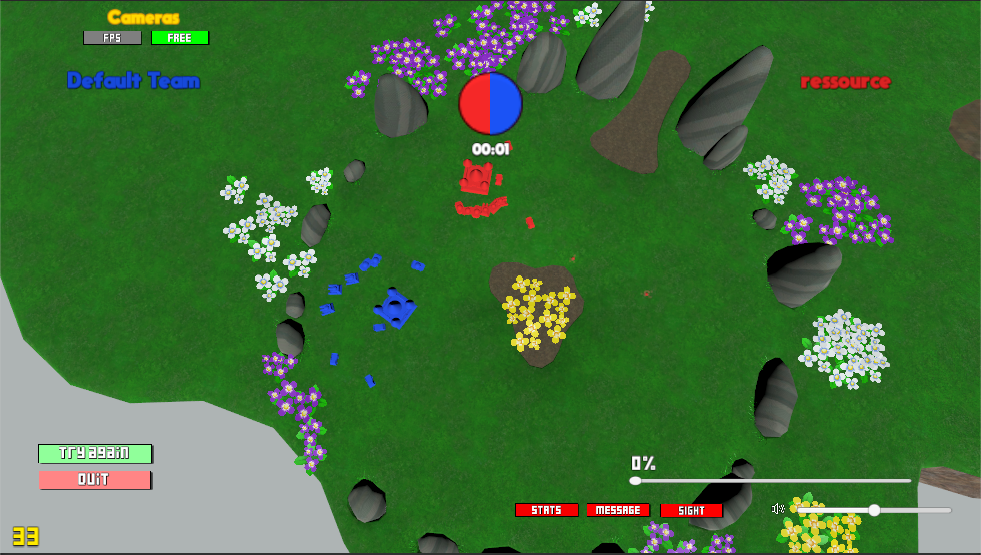
\includegraphics[scale=0.5]{DATA/warbotactuel.png}
    \\[2cm]

    \vfill
    \begin{minipage}{0.4\textwidth}
      \begin{flushleft} \large
        SAVIO Kurt \newline GALLEAN Benjamin\\

         DEAU Guillaume CHAMOULAUD Romain\\
      \end{flushleft}
    \end{minipage}
    \begin{minipage}{0.4\textwidth}
      \begin{flushright} \large
        \emph{Tuteur :} M. J \textsc{FERBER}\\
        \emph{Responsable : } M. M \textsc{LAFOURCADE}
      \end{flushright}
    \end{minipage}

  \end{center}
  \end{sffamily}
\end{titlepage}

\newpage
\tableofcontents
\newpage
% Create a new 1st level heading

\part{Présentation du projet}
\chapter{Introduction}
\section{But du projet}
\paragraph{}
L'objectif de ce projet est la réalisation d'un jeu basé sur un modèle multi-agent. L'idée générale du projet est dans la continuité de celui de l'année dernière et sur le même thème. L'outil utilisé est Unity 3D, un moteur de jeu employé dans un grand nombre de réalisations de hautes qualités. Notre projet est opérationnel sur Windows et pourrait être porté sur Mac ou encore Android.
Ce projet consiste en la réalisation d'un jeu que l'on peut qualifier de jeu pour programmeur et de permettre, notamment, à de jeunes personnes de se familiariser avec le monde de la programmation. L'utilisateur pourra donc créer un comportement pour des robots appelés "unité" afin de remplir des objectifs en jeu.
\paragraph{}
Metabot est un projet modeste réalisé à partir du logiciel Unity 3D par un groupe d'étudiants débutants dans l'utilisation de cet outil. Malgré le peu d'expérience dans la création pure de ce genre d'applications, le projet actuel est le fruit d'un travail important et d'une implication entière de toute l'équipe.
Il a donc pour unique prétention de communiquer notre amour du jeu vidéo et de la programmation.
\subsection{Cahier des charges}
Le but de notre groupe était donc l’ajout de fonctionnalités à la version Unity du jeu WarBot, tout en corrigeant ses problèmes, pour la rendre utilisable et aussi stable que possible. 
Après inspection de l’ancien projet et la nécessité de recommencer sur de nouvelles bases, nous nous sommes d’abord concentrés sur la mise en place d’un jeu générique et stable en collaboration avec le groupe MetaBot.
\paragraph{}
Le travail sur le projet a donc été réparti en 4 sous-groupes de 2 personnes comme ci : 
\begin{itemize}
\item Un groupe sur le moteur du jeu lui-même
\item Un groupe sur l’interface graphique et des interactions avec l’utilisateur
\item Un groupe travaillant sur le langage pour le comportement des unités et l’interprétation de ce langage
\item Un groupe de Game Design 
\end{itemize}

Ce rapport portera sur le sous-groupe Game Design et le sous-groupe Interpréteur, même si les groupes ont rapidement disparus afin que l’on puisse s’aider comme un groupe de 8 et que chacun puisse découvrir des parties différentes du moteur Unity 3D.
\section{Notion d'agent}
\subsection{Système multi-agents}
Un agent est une unité simple et autonome qui suit les règles donnés par un comportement  écrit par un utilisateur ou programmeur. 
Le but d’un Système multi-agent est la mise en collaboration de l’ensemble des agents dans un objectif commun, ou simplement pour observer leur évolution dans un environnement défini.
Il existe 2 types d’agents:
 Les agents cognitifs , qui disposent d’une représentation explicite de leur environnements et des agents qui les entourent. Ils disposent d’un but et peuvent s’organiser en société, tout en effectuant des collaborations si nécessaire.
Les agents réactifs répondent de manière automatique à des stimulis externe / changements dans son environnement. Cet agent n’a pas de but précis et n’est pas capable de s’organiser en société. 
Même si les agents réactifs ne sont pas organisés et capable de s’adapter à leur environnement, un ensemble d’agents réactifs sera capable d’effectuer des actions évoluées. C’est le cas d’une société d’insectes comme les fourmis par exemple. 


\subsection{Langage et comportement d’agents}
 Le langage et les échanges entre agents seront donc 2 points clés pour avoir une bonne coordination au sein d’une société.
Il est bien sûr possible d’implémenter une équipe n’utilisant aucune communication, mais les performances de l’équipe dans la réalisation de leur but seront très faible et dans le cas d’une confrontation avec une équipe organisée, leur victoire serait plus liée au hasard que de meilleures performances.

Un exemple d’agent nécessitant de la communication pour utiliser ses compétences correctement est le cas du War RocketLauncher dans WarBot , qui a une portée de tir supérieure à son champ de vision. Il va devoir s’organiser avec d’autres unités pour réussir son but.
\paragraph{}
Il existe différentes structures pour représenter le comportement d’agents : Architecture de subsomption, machine à états, … mais nous nous concentrerons sur l’Architecture de subsomption lors de ce projet, puisqu’elle est plus simple et intuitive pour de jeunes programmeurs, qui pourraient être le public cible d’un jeu comme Warbot.

Une architecture de subsomption se décompose comme un ensemble de cas que pourraient traiter l’agent, organisés de manière hiérarchique, l’ordre est donc très important.

\newpage
\chapter{WarBot: Le mode par défaut}

\paragraph{}
\begin{center}
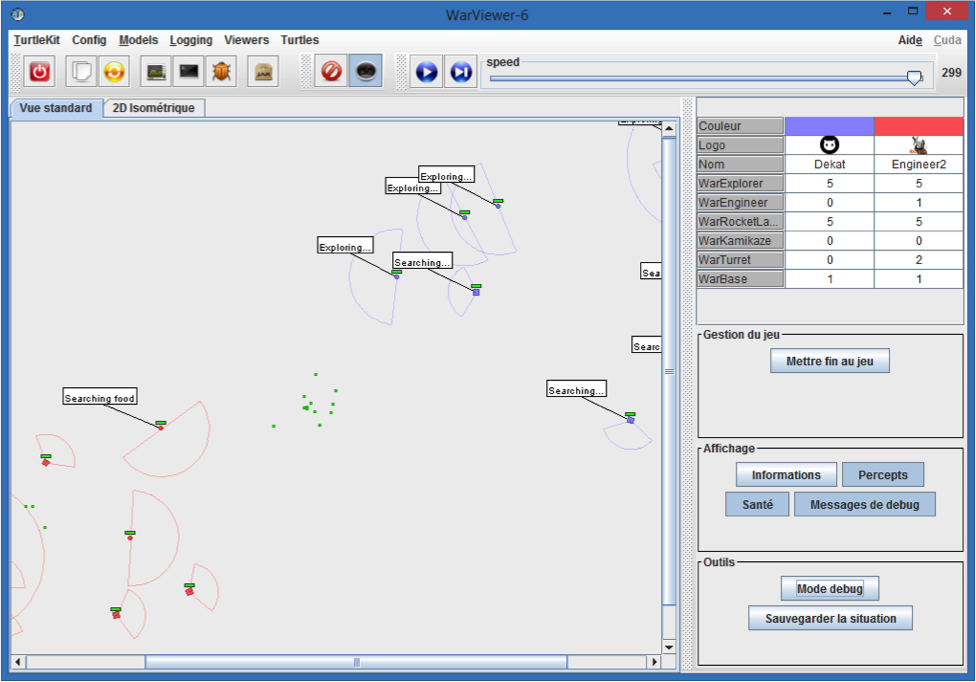
\includegraphics[scale=0.7]{DATA/warbotjava.png}
\captionof{figure} {WarBot, la version Java.r}
\end{center}
\paragraph{}

\section{Principe}
Dans WarBot, deux à quatre équipes se battent sur un terrain pour les ressources afin de survivre et d'éliminer les autres équipes afin d’être la dernière en vie. Des ressources apparaissent sur la carte et peuvent être converties en unité ou en soin.

\section{Liste des unités}
De nombreuses unités existent dans la dernière version Java de Warbot, mais nous n’avons pas pu implémenter le tout , mais nous nous sommes limités aux plus importantes, de manière à ce que le mode de jeu Warbot fonctionne.
\paragraph{}
La base :\newline
La base est l’unité la plus importante de chaque équipe. Tant qu’elle est en vie, la partie continu pour l’équipe. \newline
Elle ne peut pas se déplacer, mais elle possède un inventaire bien plus gros que les autres unités. Elle peut se soigner en utilisant les ressources que lui apporte les autres unités et peut aussi se servir de ces ressources pour créer de nouvelles unités. Il est aussi possible de créer des unités en utilisant la vie de la base.
\paragraph{}
Les explorers:\newline
Les explorers sont des unités pacifistes dans le jeu. Elles peuvent se déplacer et récupérer les ressources mais ne peuvent pas se battre.\newline
Les explorers sont la clé de la communication du jeu, car leur vitesse de déplacement élevée leur permet d’explorer, comme leur nom l’indique, la carte rapidement. \newline
Au vu de leur inventaire plus grand que la normale et leur vitesse de déplacement, ce sont les unités idéales pour rapporter les ressources à la base.
\paragraph{}
Les heavy:\newline
Les heavy sont les unités qui font le plus de dégâts du jeu. Pour compenser, ce sont les unités les plus lentes et avec la distance de vue la plus faible. \newline
Elles sont idéales pour détruire rapidement des unités immobiles.
\paragraph{}
Les light:\newline
Les light sont les autres unités offensives du jeu. Plus rapide et moins résistance que les heavy, leurs projectiles font également moins de dégâts mais leur cadence de tir est plus élevé \newline
Cette unité est très pratique pour détruire des unités mobiles. Sa rapidité lui permet de rivaliser avec les heavy qui ne devraient pas arriver à les toucher si elles se déplacent pendant l'affrontement.
\newpage
\part{Réalisation du projet}
\newpage



\newpage
\chapter{Partie "Interpreteur"}
\section{Présentation et Attente}
La partie "Interpréteur" est la partie la moins visible du projet MetaBot,
mais il s'agit de la partie du projet servant de clé de voûte du jeu.
Comme dit plus tôt, la particularité de Warbot est que le joueur, qui pourra être considéré comme le programmeur, va préparer en amont une cohésion d'équipe à travers le comportement et va pouvoir lancer un match contre une autre équipe, afin d'évaluer quel comportement sera le meilleur.
L'interpréteur permet de faire la liaison entre l'éditeur du comportement ou l'utilisateur va développer son comportement, en utilisant un ensemble d'instructions que nous avons prédéfinies  et la partie moteur, ou le fonctionnement des unités est inscrit, ainsi que les différents modes de jeux.
\paragraph{}
Le langage et l'ensemble des instructions nécessaires est alimenté par l'équipe Game Design qui nous a donné des exemples de messages ou de spécificités du langage qui pourraient être importantes. On pouvait ensuite tous en discuter en pesant le pour et le contre, afin de définir si la fonctionnalité allait être mise en place , et de quelle façon.

\section{Etude de l'ancien projet et conception préalable}

Au départ, il a été nécessaire de remettre en place un outil permettant de récupérer un comportement, qui était uniquement graphique, dans l'éditeur afin de pouvoir le renvoyer à la partie Moteur, pour que l'ensemble des unités puissent l'exécuter.
Nous avons pris connaissance de ce que l'ancien groupe avait mis en place et avons trié ce qui nous semblait correspondre à notre version du projet.
\paragraph{}
.
Il était obligatoire d'écrire le comportement reçu de l'éditeur dans un fichier, afin de le récupérer , pouvoir le modifier , le déplacer , et le conserver pour le bon fonctionnement du jeu .
La solution mise en place par l'ancien groupe pour le stockage, qui était d'utiliser un fichier XML correspondait parfaitement à notre besoin, car la syntaxe et l'organisation en nœuds de ce genre de fichiers, permettait une récupération simple et claire des instructions. Nous avons ainsi pu récupérer une partie de leur système d'écriture et de lecture de leur projet, tout en adaptant l'autre partie à nos besoins.
\paragraph{}
La partie concernant le traitement et l'exécution des instructions par les unités a dû être repensée totalement , car même si elle fonctionnait pour leur vision du jeu, était inutilisable dans l’objectif d’être générique. 
L’ensemble de la gestion de l'exécution des instructions, des droits d’accès à une primitive en fonction du type de l’unité actuelle, et la gestion des groupes étaient réalisés au sein d’un même script cumulant 2136 lignes.
\paragraph{}
Il a donc été décidé de séparer tout cela.
\paragraph{}
Le comportement d'une unité est une suite d'instructions, dont l'ordre est très important. La hiérarchie va déterminer la priorité qu'aura l'action sur le tick. Ainsi l'action la plus prioritaire dont les conditions sont acceptées sera l'action effectuée sur ce tick.
Chaque instruction est toujours organisée de la même façon :
- Une liste de conditions à remplir pour que l'instruction soit considéré comme acceptée\newline
- Une liste d'actions qui ne terminent pas le tour\newline
- L'action terminale\newline

Ce sont ces variables qui seront utilisées lors du déroulement du jeu pour exécuter les primitives correspondantes.

La gestion des différentes primitives (actions,...) à était déplacée dans la conception du moteur, pour favoriser la généricité du jeu.
\paragraph{}
Voici comment ceci a été réalisé : 

Les actions ont été représentées à part, et leur fonctionnement est simple. La base une fonction anonyme, et les différentes actions sont implémentées dans un Dictionnaire, mettant en relation un “String” correspondant au nom de l’action qu’il faut exécuter, et une fonction anonyme qui sera effectivement exécutée en jeu. Ensuite, un ensemble d’actions communes à toutes les unités seront écrites dans un script “ActionCommon” et celles-ci seront bien partagées par toutes les unités. 

\begin{lstlisting}[frame=single]
public abstract class Action : MonoBehaviour
{

    public delegate void Act();
    public Dictionary<string, Act> _actions = new Dictionary<string, Act>();
    public abstract void InitAction();
}
\end{lstlisting}

Les différences entres unités vont se faire en fonction de leur type. A partir de cet ensemble d’action commune il y a une différenciation des actions spécifiques ,des unités qui se déplacent, de la base qui est une unité assez spéciale puisqu’elle a la possibilité de créer de nouvelles unités,  un groupe d’unités qui peuvent tirer , à travers des sous classes de cette classe commune.

\begin{lstlisting}[frame=single]
public class ActionCommon : Action
{
    void Start(){
        InitAction();
    }

    public override void InitAction() {
        _actions["ACTION_IDLE"] = delegate () { };
  ...
     }
}
\end{lstlisting}

Comme dit , les actions sont ajoutées via une fonction initialisant le tableau de fonctions anonymes. Il est important que , pour chaque sous groupe d’actions, on appelle les fonctions d’initialisations de tableaux des classes mères afin que l’on récupère les actions partagées par tout le monde.
\begin{lstlisting}[frame=single]
  public override void InitAction(){
base.InitAction();
_actions["ACTION_MOVE"] 
...
}
\end{lstlisting}

\paragraph{}

Avant d'exécuter leurs actions , les unités doivent vérifier si les conditions que l’utilisateur a défini nécessaire sont bien validées. Pour cela, une structure très similaires de celles des actions a été conservée, avec le même principe de fonctions anonymes. 
Une spécificité dans la gestion des percepts (et ce sera aussi le cas pour la gestion des messages entre unités) est que l’orientation de l’unité actuelle sera modifiée selon ce qu’elle perçoit. Par exemple, si elle voit une unité agressive , elle va s’orienter vers elle, comme ça l’utilisateur ne devra pas gérer la direction de l’unité sauf si celle ci doit être orientée de manière externe (par exemple changer d’orientation si on est bloqué contre un mur).

\begin{lstlisting}[frame=single]
_percepts["PERCEPT_ENEMY"] = delegate ()
        {
            
            foreach (GameObject gO in sight._listOfCollision){
...
            GetComponent<Stats>().SetHeading(getAngle(gO));
        ...
    }
        };
\end{lstlisting}

Vers le milieu du projet, le moteur a mis en place des actions non terminales au sein du comportement des unités, puisqu’on ne pouvait plus se limiter à des actions telles que tirer ou avancer. 
WarBot étant une plate-forme multi-agents, il n’était pas concevable de ne pas mettre en place des messages entre les unités, afin de donner la possibilité au joueur d’exploiter pleinement les possibilités de coordination entre agents.

La structure des Action non terminales est la même que les Actions initiales, mais l’équipe moteur a pu installer un système permettant de les exécuter au cours de la partie, sans qu’elles ne mettent fin au tour de l’unité comme les actions “classiques”.


La dernière structure importante était donc les messages, qu’il a fallu instaurer de manière assez différente.
Ceux-ci contiennent bien sûr un expéditeur et un destinataire,mais aussi un titre qui va permettre de les différencier, pour savoir si un message va plutôt donner la position d’une ressource, une demande d’aide ou une demande d’attaque. Enfin on conservera la direction vers l’expéditeur du message, afin que le destinataire puisse se tourner facilement, à travers une action non terminale “Se tourner vers expéditeur”.

\begin{lstlisting}[frame=single]
public abstract class MessageManager : MonoBehaviour {

    public GameObject sender;
    public List<Message> _waitingMessages = new List<Message>();
    public List<Message> _currentMessages = new List<Message>();
    public string[] _messageType;
    ...
    public void UpdateMessage(){
        _currentMessages = _waitingMessages;
        _waitingMessages = new List<Message>();
    }
  }    
\end{lstlisting}

La gestion des messages dans les unités est réalisée sous forme d’une boite au lettre. Les messages qui arrivent à l’unité pendant le tick  de jeu sont stockés dans une boite “Attente” , et les messages que peuvent traiter l’unité pendant ce tick sont dans une boite “Courante”. A chaque début de tick , on va charger la boîte courante avec les messages de la boite “Attente” et on va vider la boite d’attente. Ainsi les messages ne vont pas traîner dans les boîtes de réception et ralentir le jeu. Cela implique par contre que les messages qui ne sont pas traités sont perdus, ce qui correspond bien à ce que l’on souhaite, puisqu’ainsi si toutes les ressources à un endroit ont été récupérées entre le moment où une unité envoie le message “Ressource” et que le destinataire le traite, le message n’emmenera pas l’unité à un endroit ou il n’y aura plus de ressources. De plus , il est très important que les unités ne puissent pas stocker des positions telles que la base adverse, donc pouvoir garder un message contenant la position de la base adversaire et l’utiliser alors que plus aucune unité ne se trouve près de la base adversaire est contraire à l’idée de la coordination en multi agents.
\paragraph{}

L’ensemble de ces représentations permet la séparation de l’interpréteur et de l'exécution des primitives en jeu dans le moteur, l’interpréteur sera donc totalement externe et n’aura pas besoin d’être touché lors d’ajout d’actions, conditions, messages…
De plus , cette structure utilisant les fonctions anonymes permet d'être totalement générique puisque l’ajout se fait simplement en ajoutant une entrée dans l’initialisation du tableau correspondant.
\paragraph{}



\paragraph{}
\newpage

\section{Conception et fonctionnement Interpréteur}
\paragraph{}


Le but de l'interpréteur était de traiter des fichiers de ce type :
\begin{lstlisting}[frame=single]
<behavior>
 <teamName> Default Team</teamName>
 <unit name="Explorer">
   <instruction>
   </instruction>
 </unit>
 <unit name="Base">
 </unit>
 <unit name="Light">
 </unit>
 <unit name="Heavy">
 </unit>
</behavior>
\end{lstlisting}

Ainsi nous avons un fichier par équipe écrite par l'utilisateur, chacun détaillant le comportement des unités sous la même forme :

\begin{lstlisting}[frame=single]
<behavior>
 <teamName> Default Team</teamName>
 <unit name="Explorer">
<instruction>
  <parameters>
    <PERCEPT_ENEMY />
  </parameters>
  <message>
    <ACTN_MESSAGE_HELP>
      <Light />
    </ACTN_MESSAGE_HELP>
  </message>
  <actions>
    <ACTION_MOVE />
  </actions>
   </instruction>
   <instruction>
  <parameters>
    <PERCEPT_BLOCKED />
  </parameters>
  <actions>
    <ACTION_MOVE_UNTIL_UNBLOCKED />
  </actions>
   </instruction>
 </unit>
</behavior>
\end{lstlisting}

Comme dit précédemment, l'interpréteur relie les 2 parties majeures du projet.
Ainsi, une fonction permet de transformer un fichier ".wbt" (format des équipes WarBot) vers un comportement d'équipe utilisable par l'équipe moteur, et une fonction permettant la transformation d'un comportement récupéré de l'éditeur graphique vers un fichier XML, pour sa sauvegarde.

Différentes fonctions intermédiaires ont été implémentées afin de rendre le code plus lisible et plus réutilisable.
\begin{lstlisting}[frame=single]
public Dictionary<string, List<Instruction>> xmlToBehavior(string teamName, string path)
\end{lstlisting}
Cette fonction permet d'aller lire le comportement enregistré à l'endroit du paramètres "path" , et dans le fichier appelé "teamName.wbt"

Les fichiers d'équipes sont au format XML , mais leur extension est ".wbt" pour coller au projet.

Tout d'abord, la vérification du fichier dans la fonction xmlToBehavior est un peu plus spécifique que uniquement vérifier si le fichier existe, on va aussi aller vérifier qu'on trouve bien un noeud contenant le nom de l'équipe. Cela permet d'être sûr qu'on ait un fichier de comportement, puisque le chargement des comportements est un moment clé dans le lancement du jeu.

\begin{lstlisting}[frame=single]
 if (file.Contains(Constants.xmlExtension) && !file.Contains(".meta"))
 {
        using (var stream = new FileStream(file, FileMode.Open))
        {
             if (stream.CanRead)
             {
                  Load(stream);
                  XmlNode team = SelectSingleNode("//" + Constants.nodeTeam);
                  if (team.InnerText != null && team.InnerText.Equals(teamName))
                      l_fileName = file;

                  }
             }

\end{lstlisting}


La fonction va renvoyer un dictionnaire, mettant en relation un nom de type d'unité (Explorer, WarHeavy , ....) et sa liste d'Instructions , organisé par ordre de priorité dans l'architecture de subsomption.

\begin{lstlisting}[frame=single]
XmlNodeList l_units = GetElementsByTagName(Constants.nodeUnit);
\end{lstlisting}

Ici on récupère les listes des noeuds par unité, ainsi que tous les noeuds fils que l’on devra lire.
Pour chacun des noeuds d'unités, on va faire appel une fonction intermédiaire, “xmlToUnitBehavior”, qui va renvoyer le comportement de cette unité, dans le fichier que traite la fonction principale.
Celle-ci va renvoyer une liste d’instructions correspondante à l’unité passée en paramètres, en faisant appel à la fonction coeur de l’interpréteur.

\begin{lstlisting}[frame=single]
public override Instruction whichInstruction(string unitName, XmlNode ins)
\end{lstlisting}

Cette fonction va récupérer le noeud qu'on va lui passer dans la fonction "xmlToUnitBehavior", et va aller construire chaque instruction grâce à l'ensemble des fils du noeud "ins".
Il est très avantageux de pouvoir utiliser un noeud pour contenir tout le comportement pour une unité précise ici, puisque le parcours de ces fils est simple et formaté en XML. 
On va ainsi parcourir tous les cas qui nous intéressent  et remplir une Instruction qui sera renvoyée à la fonction “xmlToUnitBehavior”.
Les cas sont les suivants :\newline
Parcours de l’ensemble des noeud ayant comme intitulé “parameters”, qui correspondent au conditions de l’instruction, et stockage du nom du noeud, qui sera la clé du tableau du moteur pour exécuter la condition.\newline
Parcours de l’ensemble des noeud ayant comme intitulé “message”, qui correspondent au actions non terminale et messages l’instruction, et stockage du nom du noeud, qui sera la le type de message. On va aussi conserver le nom du noeud enfant de ce message, qui correspond au destinataire du message. Dans le cas d’une action non terminale, ce noeud sera inutilisé\newline
Ce message ne sera pas traité comme un “String”, mais comme une structure “MessageStruct” du moteur.\newline
Parcours du noeud ayant comme intitulé “action”, qui correspondent à l’action qui terminera l’instruction, et stockage du nom du noeud, qui sera la clé du tableau du moteur pour exécuter l’action.\newline

 La fonction “xmlToUnitBehavior” n’aura plus qu'à construire une liste de ces instructions au fur et à mesure du parcours des noeuds , et mettre en relation la clé , le nom de l’unité , et la valeur , la liste d’instructions, dans le Dictionnaire résultat.
\paragraph{}
Vous pourrez retrouver cette fonctionne en annexe, à la figure 6.1
\paragraph{}
Nous avons vu ici le traitement du cas ou on souhaitait récupérer des comportements depuis un fichier pour le renvoyer sous une suite d’instructions. Cette fonction est vitale pour le fonctionnement du moteur, mais elle sert aussi du côté de l’éditeur de comportement pour pouvoir charger un fichier dans la zone des pièces de puzzle.

Il est donc bien sûr important de pouvoir faire le chemin inverse, et donc d’écrire un comportement au format XML depuis un ensemble d’instructions récupérées depuis l’éditeur.

\paragraph{}

Cette partie sera plus facile à réaliser que la précédente 
L’idée ici est de stocker la structure XML de chaque instruction dans la classe Instruction même , mais pas dans une variable , plutôt dans une fonction qui va nous renvoyer le noeud XML correspond à ladite instruction. Ainsi il faudra juste ajouter ce noeud au reste du fichier de l’équipe puis le sauvegarder.

Pour chaque unité, on va créer un nouveau noeud , ou vider l’ancien si le noeud existait déjà, puis on va construire la structure de l’unité grâce à la fonction renvoyant un noeud XML de chaque instruction. 
Voici à quoi ressemble cette fonction renvoyant la structure XML :
\begin{lstlisting}[frame=single]
 public XmlNode xmlStructure()
    {
        XmlDocument l_doc = new XmlDocument();
        XmlNode l_ifNode = l_doc.CreateElement("instruction");

        XmlNode paramNode = l_doc.CreateElement("parameters");
        foreach (string c in _listeStringPerceptsVoulus)
        {
            XmlElement t = l_doc.CreateElement(c);
            paramNode.AppendChild(t);
        }
        l_ifNode.AppendChild(paramNode);

        if (_stringActionsNonTerminales.Length > 0)
        {
            XmlNode MsgNode = l_doc.CreateElement("message");
            foreach (MessageStruct c2 in _stringActionsNonTerminales)
            {
                XmlNode t2 = l_doc.CreateElement(c2._intitule);
                XmlNode t2d = l_doc.CreateElement(c2._destinataire);
                t2.AppendChild(t2d);
                MsgNode.AppendChild(t2);
            }

            l_ifNode.AppendChild(MsgNode);
        }

            XmlNode actNode = l_doc.CreateElement("actions");
        if (_stringAction != "")
        {
            XmlNode a = l_doc.CreateElement(_stringAction);
            actNode.AppendChild(a);

            l_Node.AppendChild(actNode);
        }

        return l_ifNode;
    }
\end{lstlisting}

La construction de la structure XML est rapide, il suffit de parcourir les percepts et les actions non terminales et de construire les noeuds que si elles sont présentes, on va ensuite construire un dernier noeud étant l’action finale , celle-ci étant obligatoire.

Nous avons ici fait le tour des possibilités de l’interpréteur, nous avons vu les représentations des primitives des unités, et comment l’interpréteur a répondu aux besoin du projet. 

A partir de ce moment du projet, l’équipe Interpréteur est devenue plutôt libre puisque le plus important était d’aider les autres équipes dans l’avancée de leur partie. De nouveaux travaux allaient être donnés à l’équipe, mais dans les moments d’attente, chacun apportera son aide ailleurs dans le jeu.

\newpage
\paragraph{}

\section{Internationalisation du projet}

Un nouveau travail d'interprétation a vite été ressenti dans le projet. En effet, le jeu étant destiné à aider les jeunes à appréhender la programmation, une traduction française était nécessaire.
Toujours dans l'idée de rester générique, un traducteur a été mis en place et attaché à l'ensemble des textes qui seront affichés à l'utilisateur. L’idée était de pouvoir rattacher rapidement la traduction dès l’ajout de textes et aussi de pouvoir rajouter des langues de manière externe.

\paragraph{}
\subsection{Mise en place}

Dans les fichiers du jeu , on retrouve un dossier contenant ces traductions,sous formes de fichier représentant chacun une langue.
Une traduction est simplement une ligne du fichier mettant en relation une clé et sa traduction.
Le rajout d'une langue est totalement simple et générique :
On ajoute un fichier ayant le nom de la langue que l'on souhaite, et qui doit obligatoirement implémenter l'ensemble des clés présentes dans les autres fichiers, ou dans le fichier "example" mis à disposition.

Voici à quoi ressemble les fichiers de traduction :
\begin{lstlisting}[frame=single]
# Percepts
  PERCEPT_ALLY=PERCEPT_ALLIE_A_PORTEE
  FALSE_PERCEPT_ALLY=PERCEPT_AUCUN_ALLIE_A_PORTEE
  PERCEPT_IS_NOT_LOADED=PERCEPT_PAS_RECHARGE
  FALSE_PERCEPT_IS_NOT_LOADED=PERCEPT_EST_RECHARGE
# Map en jeu
  Recommencer=Recommencer
  Quitter=Quitter
  Health : =Vie :
  Bag : =Sac :
  Heading : =Orientation :
  Contract :=Contrat :
\end{lstlisting}

On peut voir que le caractère séparateur est le caractère ' = ' , au départ nous utilisions le caractère ' : ' , mais il y a eu des conflits puisque les textes affichés sur l'interface utilisateur contiennent aussi les ':'.
Il est possible que le caractère ' = ' pose problème au bout d'un moment, si jamais des traductions ajoutées ultérieurement le contiennent. Il faudra donc simplement faire une recherche "Trouver et Remplacer" dans les fichiers de traduction, et changer un seul caractère dans le code du Parser des fichiers de traductions.

\paragraph{}

La traduction dupliquée de chaque texte comme vue dans la partie "Percepts" de l'exemple plus haut, à laquelle on ajoute un "FALSE\_" , provient du fait que les conditions qui sont traitées dans le jeu peuvent être mises au négatif. Par exemple, si le comportement d'une unité de mon équipe cherche à savoir si cette unité à "un contrat d'élimination en cours" lorsqu'elle reçoit le message demandant de l'aide depuis la base, il est tout à fait possible que l'on cherche à vérifier que l'on a aucun contrat d'élimination pour pouvoir en accepter un nouveau.
Au lieu de dupliquer les conditions dans le code , il a été préféré de pouvoir les rendre négatives.
\paragraph{}
La traduction fonctionne ainsi :
Un premier script,le LangageLoader s'occupe de vérifier la langue qui doit être utilisée dans le fichier de configuration du jeu et va charger en mémoire un fichier  de traductions.
Ce script va aller chercher la langue qui doit être appliquée au projet dans les fichiers de configuration du jeu à son initialisation, et va récupérer les traductions en lisant le fichier correspondant à la langue souhaitée. 
Deux structures de données ont été mises en place pour faciliter les traductions 
\begin{lstlisting}[frame=single]
[System.Serializable]
public struct Traduction
{
    public string cle;
    public string valeur;

}
\end{lstlisting}

La première est une Traduction , qui va mettre en relation une clé qui sera le texte initial contenu dans les boutons et textes du projet, et une traduction qu’il faudra afficher. Ce sont les mêmes clés valeur qui seront parsés dans le fichiers de traduction. 

L’appel “System.Serializable” va permettre à Unity de transformer cette structure de données dans un format que le moteur peut stocker et reconstruire si il y en a besoin. C’est par exemple le cas pour l’affichage des traductions dans l’inspecteur de Unity, ce qui a permis de grandement faciliter le débogage de ces fonctionnalités. 


\begin{lstlisting}[frame=single]
[System.Serializable]
public struct Langage
{
    public string langue;
    public List<Traduction> trads;
}
\end{lstlisting}

Ceci est la structure qui va permettre de conserver une langue, représentée simplement comme un ensemble de traductions.
\paragraph{}
Il est théoriquement possible de stocker plusieurs langues à la fois dans le “LangageLoader”, mais  on va vider la liste des traductions à chaque fois que la langue est modifiée dans les paramètres, pour ne pas stocker trop de choses en runtime.

 Ce script est rattaché à un objet des scènes Unity appelé le Game Manager,qui a été mis en place par l’équipe moteur et n’est pas détruit au changement des scènes.Le fait que cet objet soit conservé à travers les scènes provient d’utilisation de l’appel “DontDestroyOnLoad()” . Ainsi, si il y a besoin de partager des ressources entre les scènes tel que des configurations , ont peut utiliser le GameManager. 

\paragraph{}
\begin{center}
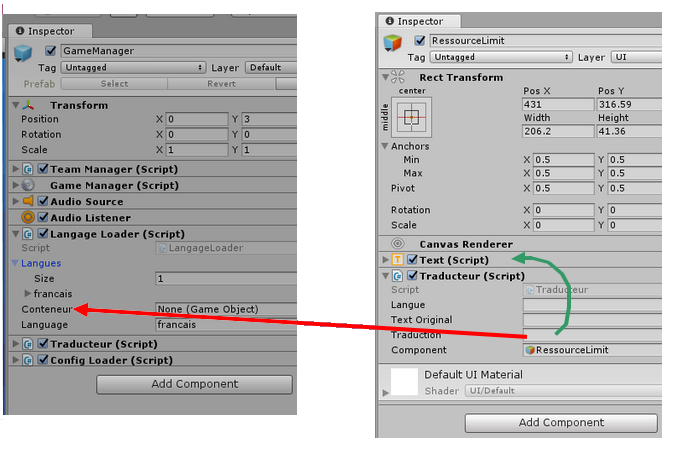
\includegraphics[scale=0.7]{DATA/traducteur2.png}
\captionof{figure} {Intéraction Traducteur/Objet - GameManager}
\end{center}
\paragraph{}


Un second script est lui attaché à tous les Objets du jeu qui vont devoir être traduits. Celui-ci va , à la création de l'objet auquel il est rattaché, chercher la langue actuellement affichée, récupérer comme clé le texte original de l'objet auquel le script est affilié, et va stocker la traduction récupérée dans le LangageLoader du GameManager, et l'afficher à l’utilisateur.

\begin{lstlisting}[frame=single]
   public void Traduction()
    {
        foreach (Langage l in GameObject.Find("GameManager").GetComponent<LangageLoader>().langues){
            if (l.langue.Equals(langue)){
                foreach (Traduction t in l.trads){
                    if (textOriginal.Equals(t.cle)){
                        traduction = t.valeur;
                        return;
                    }
                }
            }
        }

        traduction = textOriginal;
    }
\end{lstlisting}

En Runtime, si la langue est changée dans les paramètres du jeu, les script de traduction des objets vont mettre à jour leur langue, et récupérer la nouvelle traduction dans le "GameManager".

\begin{lstlisting}[frame=single]
void Update () {
            if (gameManager.GetComponent<LangageLoader>().language != langue){
            langue = gameManager.GetComponent<LangageLoader>().language;
            Traduction();
            if (component)
                component.gameObject.GetComponent<Text>().text = traduction;
            }
}
\end{lstlisting}

\paragraph{}
La traduction est aussi disponible sans rattacher un script "Traducteur" à un Objet de la scène.
En effet, il y a beaucoup de situations ou on ne peut pas rattacher ce script. Pour cela, une instance du traducteur a été placée dans le GameManager, pour qu'on puisse accéder à une traduction.
La fonction setTextOriginal() du traducteur se charge donc de changer le texte à traduire puis appliquer la traduction.

Un des endroits qui nous a forcé à pouvoir utiliser le traducteur autrement qu’en étant rattaché à un objet de la scène est le cas des pièces de puzzle.
En effet celle-ci ne sont pas dans la scène au lancement du jeu mais sont générées dynamique en fonction des interactions de l’utilisateur dans l’éditeur de comportement. 
On ne pouvait donc pas leur rattacher un traducteur.

\paragraph{}
\begin{center}
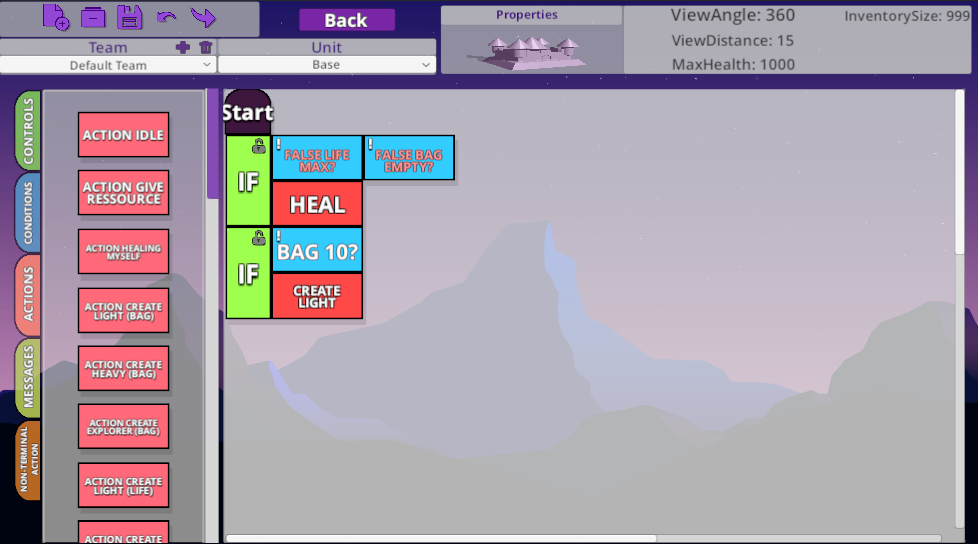
\includegraphics[scale=0.5]{DATA/piecetrad.png}
\captionof{figure} {Traduction en anglais des pièces de puzzle}
\end{center}
\paragraph{}


La langue actuelle est conservée dans un fichier de configuration, pour que le projet conserve la langue au changement de scène et quand on relance le jeu.

\paragraph{}
\begin{center}
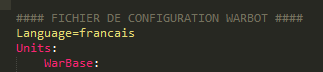
\includegraphics[scale=0.9]{DATA/fichierconfig.png}
\captionof{figure} {Fichier configuration}
\end{center}
\paragraph{}

Mais ce fichier est caché, à moins de connaître sa position dans la hiérarchie et de devoir redémarrer le jeu pour changer la langue,il vaudra mieux utiliser les 2 boutons sont dans les paramètres pour passer en Français ou en Anglais. Si le besoin de nouvelles langues se fait sentir dans le futur, il sera toujours possible de transformer ces boutons en un "DropDown" , un menu déroulant, afin de pouvoir sélectionner autant de langues que disponible.

\paragraph{}
\begin{center}
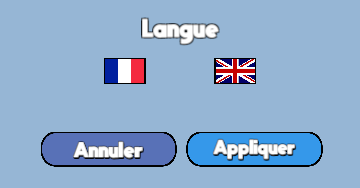
\includegraphics[scale=0.8]{DATA/langue.png}
\captionof{figure} {Boutons changement de langues}
\end{center}
\paragraph{}
\newpage


\section{Caméras Spécifiques}

Depuis le début de l’existence de WarBot,les caméras ont toujours été des caméras vue de dessus, puisque ce genre de caméras correspond parfaitement à la vue globale que l’on cherche à avoir pour regarder les agents évolués sur le terrain.
Nous n’allions pas déroger à la règle et avons conservé cette caméra vue de dessus, mais une spécificité à été implémentée par l’équipe moteur qui est une caméra qui va suivre le mouvement moyen des unités afin d'être toujours orienté vers l’action. 

Le script va simplement calculer la moyenne des positions de l’ensembles des unités sur le terrain, et va déplacer l’angle de la caméra vers cette position moyenne , grâce à la fonction “LookAt” contenue dans les caméras de Unity. 

\begin{lstlisting}[frame=single]
     Vector3 res = Vector3.zero;
     GameObject[] units = GameObject.FindGameObjectsWithTag("Unit");

     foreach (GameObject go in units)
      {
          res += go.transform.position;
      }
      res *= 1f / (units.Length + 1);
      currentTarget += (res - currentTarget) * Time.deltaTime * _speed;
       transform.LookAt(currentTarget);
\end{lstlisting}

\subsection{Caméra première personne}
\paragraph{}

Sur une idée de notre encadrant M. Ferber, il a été décidé de mettre en place une caméra première personne , car cette option permettait à l’utilisateur de se mettre dans la vue complète de l’unité et de pouvoir mieux suivre ce qui peut se passer autour de cette unité, et pour profiter pleinement des possibilités que permet une version Unity du jeu. \newline

Un premier jet de la caméra avait été une caméra totalement dans l’unité, suivant ainsi sa position et sa rotation. La caméra était en soit très bien , mais le fait de suivre la rotation de l’unité était peu agréable car les unités ont tendance à beaucoup bouger et se retourner dans les coins. 

D’autres essais ont été réalisés, telle qu’une caméra centrée au dessus de l’unité. On pouvait ainsi voir ce qui se déroulait autour de l’unité , tout en suivant sa position mais pas sa rotation. Idée s’éloignant trop de l’idée de caméra première personne, l’équipe est revenu sur une caméra première personne , tout en cherchant un moyen de ne pas subir les changements de rotation des unités. 
\paragraph{}
La caméra première personne finale est donc située sur le capot de l’unité, mais la rotation de celle ci est déterminée par les mouvements de souris de l’utilisateur. L’utilisateur peut donc observer ce qui se passe autour de lui , tout en suivant l’unité. 

\paragraph{}
\begin{center}
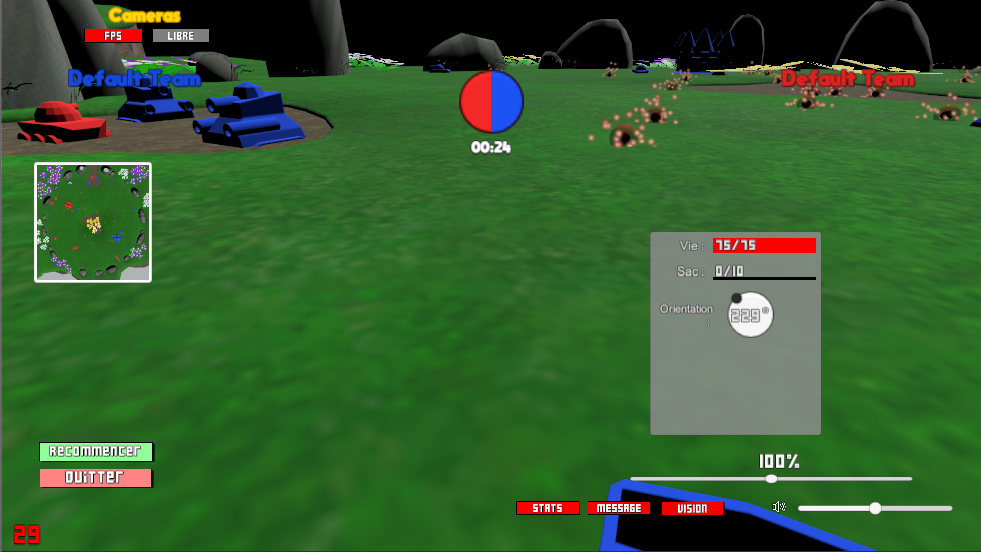
\includegraphics[scale=0.6]{DATA/camerafps.png}
\captionof{figure} {Vue “FPS” dans l’unité}
\end{center}
\paragraph{}


On peut aussi remarquer l’apparition d’un petit HUD sur la droite, qui n’est présent que lorsqu’on est en caméra première personne, et qui correspond à l’unité à laquelle on est “rattaché”. On peut y voir la vie actuelle/max de l’unité, sa quantité de ressource dans le sac, son orientation pour du débug.
Il y a aussi sur la gauche une mini carte qui apparaît uniquement en caméra fps, qui permet à l’utilisateur de suivre l’action de manière globale sur la carte de jeu tout en étant en Vue première personne. 

Cette mini carte a pu être mis en place avec Unity, puisqu’avec la possibilité de placer une caméra assez haut dans les scènes des cartes du jeu , puis le rendu de cette caméra est redirigé dans une texture. Puis il suffit d’appliquer cette texture à une image , pour que cette image rende en temps réel la carte vue de dessus. 
On a pu ajouter un cadre à mini carte pour ne pas la confondre avec le sol. 

\paragraph{}
\begin{center}
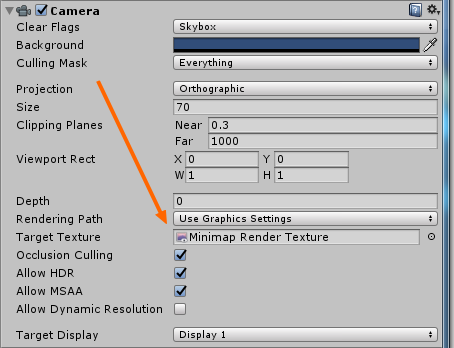
\includegraphics[scale=0.6]{DATA/textureminimap.png}
\captionof{figure} {Caméra enregistrant dans une texture}
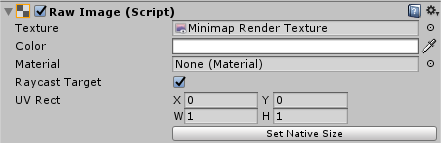
\includegraphics[scale=0.7]{DATA/imageminimap.png}
\captionof{figure} {Image affichant une texture}
\end{center}
\paragraph{}

\subsection{Caméra “Libre”}

Au final, une nouvelle caméra à été ajouté au projet, qui a été inspirée de jeux tel que Age of Empires, Civilisation ou Dota, qui est une caméra qui laisse la liberté à l’utilisateur de se déplacer et de dézoomer ou zoomer à l’utilisateur. Nous avons bien sûr bloqué la caméra sur les côtés de la carte pour éviter que l’utilisateur puisse se déplacer tant qu’il le souhaite d’un côté ou de l’autre.
Une limite à aussi été mise en place sur le zoom/dézoom en caméra libre, de telle manière qu’on ne voit pas la fin de la carte sur unity, mais aussi qu’on ne puisse pas traverser les objets en zoomant trop. 

Le zoom est très classique, il suffit de scroller vers l’avant avec la souris pour zoomer et dans le sens inverse pour dézoomer. Pour les déplacements de la caméra, tant que la souris est dans l’écran la caméra ne bouge pas , et dès que la souris sort de l’écran la caméra va suivre la direction de la souris que ce soit sur le côté ou en diagonale.
\begin{lstlisting}[frame=single]
 if (Input.mousePosition.x <= 2 && Camera.main.transform.position.x > backPosition.x - terrain.bounds.size.x / 4)
     Camera.main.transform.position = new Vector3(Camera.main.transform.position.x - speed, Camera.main.transform.position.y, Camera.main.transform.position.z);
if (Input.mousePosition.y <= 2 && Camera.main.transform.position.z > backPosition.z - terrain.bounds.size.z / 4)
         Camera.main.transform.position = new Vector3(Camera.main.transform.position.x , Camera.main.transform.position.y , Camera.main.transform.position.z - speed);

if (Input.mousePosition.x >= Screen.width - 2 && Camera.main.transform.position.x < backPosition.x + terrain.bounds.size.x / 4)
        Camera.main.transform.position = new Vector3(Camera.main.transform.position.x + speed, Camera.main.transform.position.y, Camera.main.transform.position.z);
if (Input.mousePosition.y >= Screen.height - 2 && Camera.main.transform.position.z < backPosition.z + terrain.bounds.size.z / 4)
         Camera.main.transform.position = new Vector3(Camera.main.transform.position.x, Camera.main.transform.position.y , Camera.main.transform.position.z + speed);
 \end{lstlisting}

\paragraph{}
Comme vous le voyez , on va se limiter à maximum un quart de la taille du terrain de la scène sur chaque côté, afin de ne pas trop dépasser la scène.
\paragraph{}
La gestion des deux caméras se fait à travers un système d’états gérés par des boolean, et les déplacements de la caméra s’adaptent à l’état dans lequel on se trouve.
Des changements d’états sont possibles mais il sont limités. En effet , passer d’une caméra première personne à une caméra troisième personne sans repasser par la caméra initiale ne va pas fonctionner.  On risque de se retrouver à se déplacer tout en étant collés au sol.

L’utilisateur peut choisir sa caméra directement depuis le HUD en jeu,  a partir de 2 boutons qui vont suivre les états des caméras.

\paragraph{}
\begin{center}
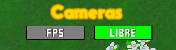
\includegraphics[scale=1]{DATA/cem.png}
\captionof{figure} {Configuration à l’état initial}
\end{center}
\paragraph{}

Initialement, on ne peut passer qu’en caméra libre à partir des boutons, puisque le passage en caméra première personne se fait en cliquant directement sur l’unité voulue.
Lorsque le bouton est vert, cela signifie que l’on peut cliquer dessus pour passer sur la caméra correspondante. Si il est rouge cela signifie que l’on peut cliquer dessus pour quitter la caméra actuelle et revenir dans l’état initial. 
Enfin si il est grisé, cela signifie que cette caméra n’est pas disponible dans ce mode

\paragraph{}
\begin{center}
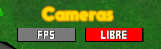
\includegraphics[scale=1]{DATA/Sanstitre3.png}
\captionof{figure} {Bloquage de la caméra libre en première personne}
\end{center}
\paragraph{}
\newpage


\section{Fin du jeu et Statistiques}

Avec la quantité de travail pour faire fonctionner le moteur, un écran de fin du jeu n’avait pas encore mis en place,alors qu’il totalement vital ici. Si l’on souhaite que WarBot soit utilisable l’année prochaine pour l’UE Programmation Orientée Agents de M. Ferber, il est nécessaire de pouvoir finir le jeu et récupérer le nom du gagnant du match.
\paragraph{}
La aussi dans l’optique d’une généricité maximale, il a fallu trouver un moyen de pouvoir ajouter très facilement des conditions et des exécutions de fin.
Nous nous sommes ainsi inspirés du fonctionnement des Actions, et  utilisons ainsi des fonctions anonymes stockées dans 2 tableaux. 
Le EndGameManager doit pouvoir vérifier à chaque tick du jeu si la condition de victoire actuelle est validée, et si c’est le cas on va exécuter une séquence d’instructions détaillées plus tard.

\begin{lstlisting}[frame=single]
void Update()
    {
        if (_tests[_wincondition]())
            _ends[_wincondition]();
    }
\end{lstlisting}
\paragraph{}

On va donc initialiser les tableaux à la création du script, ainsi que récupérer la condition de victoire choisie par l’utilisateur.

Il  a ensuite fallu montrer à l’utilisateur que le jeu était bien fini, ce qui nous a permis de découvrir l’animation avec Unity. Il s’agira ici que d’animation très simple. 

L’animateur dans Unity va récupérer des objets de la scène et on va pouvoir appliquer des transformations à différentes propriétés de ces objets au fur et à mesure du temps. 

\paragraph{}
\begin{center}
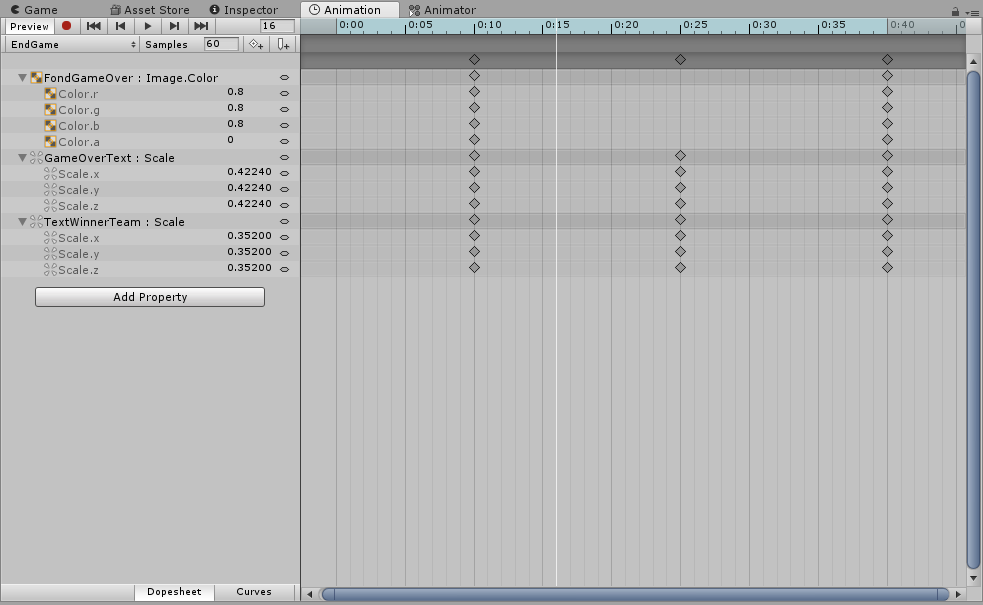
\includegraphics[scale=0.5]{DATA/animation.png}
\captionof{figure} {Exemple d’animation dans Unity}
\end{center}
\paragraph{}


Sur la photo ci-dessus, nous voyons sur la gauche les différents objet impliqués dans l’animation , et l’écoulement du temps sur le milieu. 
Il est possible d’ajouter des images clés sur la timeline, et définir les valeurs qu’auront les  propriétés des objets à chaque image clé. Par exemple, si à 10 secondes je veux que la taille de mon texte soit à 100\% je vais simplement mettre une frame sur 10 sec, et mettre la valeur 1 dans la propriété “Scale” du texte. Unity va donc augmenter linéairement la taille de mon texte entre 0 et 10 secondes.\newline
L’animation ici correspond à l’apparition d’un fond coloré , avec une augmentation progressive de sa transparence sur le temps de l’animation. Par dessus, on va voir 2 textes contenant le mot “Game Over” et aussi le nom de l’équipe gagnante. Ces 2 textes vont grossir de 0 à 1.2x leur taille initiale pour ensuite revenir à 1x la taille initiale, pour ajouter un peu de dynamique à l’animation.
\paragraph{}
Une fois l’animation terminée, il faut déterminer quand a t-on besoin de jouer cette animation et certains paramètres (doit elle boucler ? , …)
Ici , il ne fallait absolument pas que l’animation boucle, l’écran doit rester fixe lorsque le jeu est fini. Il est donc indispensable de simplement jouer l’animation dès qu’on détecte la fin du jeu. 
\paragraph{}
Unity possède un bon outil pour gérer les états des animations, il s’agit d’une machine à état, qui va pouvoir faire passer le jeu d’un état à un autre en fonction de “triggers” , que le développeur peut appeler dans un script. 

\begin{center}
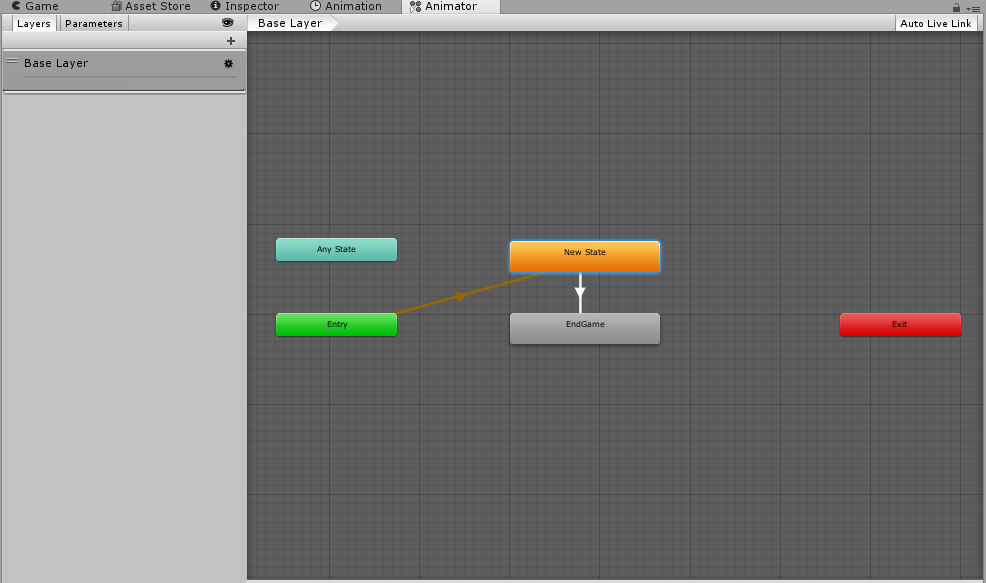
\includegraphics[scale=0.5]{DATA/machineetat.png}
\captionof{figure} {Machine à états Unity}
\end{center}
\paragraph{}

Ici, le jeu se trouve dans l’état orange lors de son déroulement. Cet état est juste ici en attente de la fin du jeu et ne fait rien d’autre. 
La transition entre l’état orange et l’état gris est appelé lorsque le trigger “Gameover” est activé. Arrivé dans l’état gris, Unity va jouer l’animation de fin du jeu , mais nous avons défini qu’elle ne devait pas boucler , donc les textes vont ainsi rester affichés sur l’écran.
La transition vers l’état Exit ne doit pas être faite, sinon l’utilisateur ne pourra pas rester sur l’écran de fin du jeu.
\begin{lstlisting}[frame=single]
anim.SetTrigger("GameOver");
\end{lstlisting}

Cet appel doit être réalisé après avoir relié l’animation avec le script en utilisant la variable “anim”

Au final, le fond coloré à été retiré de l’animation pour laisser simplement les 2 textes blancs, car ce fond empêche l’utilisateur de voir l’état de la partie à la fin du jeu, et donc voir quelles unités il reste, ou à quel point la partie était serrée / unilatérale. Voici une image de l’écran de fin du jeu.
\paragraph{}
\begin{center}
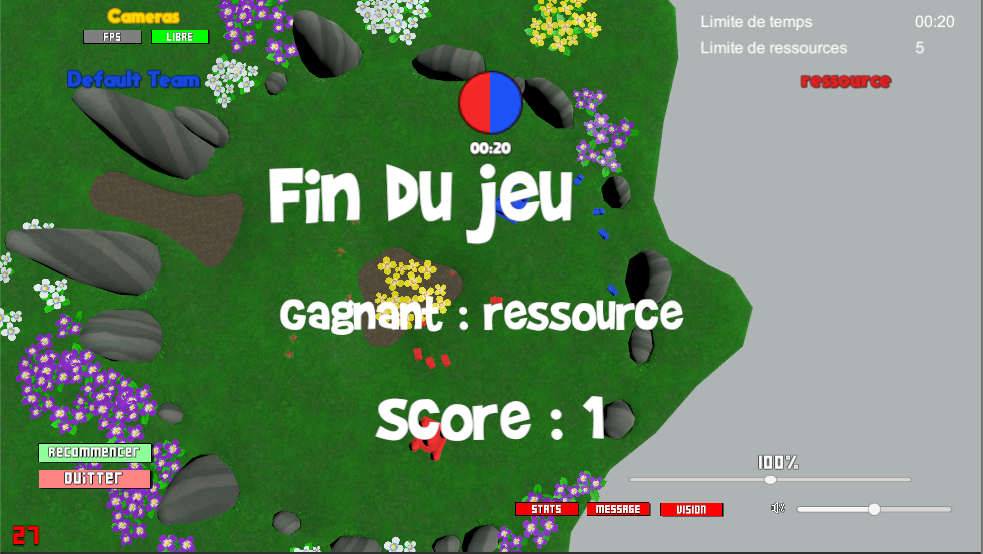
\includegraphics[scale=0.5]{DATA/findujeu.png}
\captionof{figure} {Écran après l’animation}
\end{center}
\paragraph{}


La gestion de la fin du jeu de chaque mode doit intégrer au moins 2 appels obligatoires. Le premier est l’activation du trigger “Gameover” déclenchant l’animation et le second étant les appels aux scripts d’enregistrement du score des équipes.


% classements des équipes ELO + Matchups
\section{Score des équipes}

\subsection{Match-up}
Les match-up permettent d'enregistrer les différents match entre équipes afin de pouvoir afficher les résultats (victoire et défaite) d'une équipe par rapport à une autre. Chaque équipe à un fichier .stat créé lors de la création d'équipe et est modifié à chaque fin de match. le format de ce fichier est 
\[
TeamName/MatchCount/WinCount
\]
\paragraph{}
A la fin d'un match, les fichiers de chaque équipe sont modifié afin de mettre à jour ces statistiques. \newline
Pour cette mise à jour, pour chaque équipe adverse, 2 cas sont possible :
\newline
\begin{itemize}
\item
les équipes se sont déjà affronté avant
on recherche, dans la liste des équipes affrontées, l'équipe adverse actuelle et on incrémente MatchCount. Si l'équipe actuelle est l'équipe gagnante, on incrémente aussi WinCount
\begin{lstlisting}[frame=single]
int numVal = int.Parse(DetailStat[1]);
numVal++;
DetailStat[1] = numVal.ToString(); //NbMatch
if (Team == Winner)
{
    numVal = int.Parse(DetailStat[2]);
    numVal++;
    DetailStat[2] = numVal.ToString(); //NbVictoire
}
\end{lstlisting}
\item
les équipes ne se sont jamais affronté
on ajoute une ligne au fichier tel que TeamName/1/0. cette ligne sera TeamName/1/1 si l'équipe actuelle est l'équipe gagnante
\begin{lstlisting}[frame=single]
i++; //taille du tableau + 1
System.Array.Resize(ref Stats, i);
if (Team == Winner) 
    Stats[i-1] = Teams[0] + "/1/1";
else 
    Stats[i-1] = Teams[0] + "/1/0";
\end{lstlisting}
\paragraph{}
\end{itemize}
Les match-up étaient affichés sur l'écran d'accueil. Cependant, prenants trop de place, ils ont été effacés de l'écran d'accueil et pourraient être affichés sur une fenêtre à part si l’équipe qui va récupérer le projet le souhaite.


\subsection{Système de points ELO}

Le système ELO est un système de classement par niveau de capacité relatif d'un joueur pour les jeux à deux joueurs. Pour WarBot, ce système sert à évaluer les capacités d'une équipe complète afin de pouvoir estimer ses performances en combat 1 contre 1. 
\paragraph{}
La formule permettant de calculer le ELO d'un joueur à l'issue d'un match est 
\[
E_{n+1} = E_n + K * (W - p(D))
\]
\paragraph{}
p(D) est la probabilité de gain par rapport à la différence du ELO des deux joueurs. il peut s'exprimer sous la forme
\[ 
p(D) = \frac{1}{1 + 10^{\frac{-D}{400}}}
\]
\paragraph{}
D est la différence entre le ELO du joueur et le ELO du joueur adverse
\[
D = E_{Joueur 1} - E_{Joueur 2}
\]
\paragraph{}
W est le résultat du match. en cas de victoire W = 1, en cas de défaite W = 0 et en cas d'égalité W = 0.5
\paragraph{}
K est un facteur dépendant de la volatilité du classement et permet d'amplifier les variations afin que les nouveaux joueurs progressent rapidement vers le réel niveau. Pour WarBot, nous avons utilisé les coefficients suivant
\[
K = 80 \iff ELO < 1000 
\]
\[
K = 50 \iff 1000 <= ELO < 2000
\]
\[
K = 30 \iff 2000 <= ELO < 2400
\]
\[
K = 20 \iff ELO >= 2400
\]
\paragraph{}
$E_n$ est le ELO du joueur avant le match.
\paragraph{}
Lors de la création d'une équipe, nous mettons le ELO de cette équipe à 2400. Ce choix réduit cependant les variations dû à K. En effet, K sera à 30 dès lors du premier match d'une équipe mais sera élevé pour une équipe faible afin qu'elle remonte vite en cas de victoire face à une équipe plus haute.
\paragraph{}
\newpage
Exemple : \newline
L'équipe 1 avec un ELO de 1800 affronte l'équipe 2 avec un ELO de 2550 \newline
Les probabilités de gain des deux équipe sont
\[
p_{Equipe 1}(D) = 0.01
\]
\[
p_{Equipe 2}(D) = 0.99
\]\newline

Les facteurs K des deux équipe sont 
\[
K_{Equipe 1} = 50
\]
\[
K_{Equipe 2} = 20
\]\newline
N'ayant pas d'égalité dans WarBot, les possibilités sont les suivantes :
\newline
\begin{itemize}
\item
L'équipe 1 gagne.
\[
E_{Equipe 1 n+1} = 1800 + 50 * (1 - 0.01) = 1800 + 50 *  0.99 = 1800 + 49 = 1849
\]
\[
E_{Equipe 2 n+1} = 2550 + 20 * (0 - 0.99) = 2550 + 20 * -0.99 = 2550 - 19 = 2531
\]
\newline
\item
L'équipe 2 gagne.
\[
E_{Equipe 1 n+1} = 1800 + 50 * (0 - 0.01) = 1800 + 50 * -0.01 = 1800 - 0 = 1800
\]
\[
E_{Equipe 2 n+1} = 2550 + 20 * (1 - 0.99) = 2550 + 20 *  0.99 = 2550 + 0 = 2550
\]
\end{itemize}
\paragraph{}
Suite à ce calcul, les résultats sont stockés dans des fichiers .ELO afin de pouvoir le re-calculer le ELO à la fin de chaque match et de l'afficher dans un classement.

\subsection{Affichage}
Les points ELO des équipes ainsi stockés vont pouvoir être récupérés à chaque fois qu’une équipe va être sélectionnée sur le menu principal , on va afficher son score ELO juste en dessous, en appliquant une teinte, selon si le ELO est supérieur à la valeur initiale (teinte plutôt verte) ou inférieure (teinte plutôt orange).

Voici un exemple 

\paragraph{}
\begin{center}
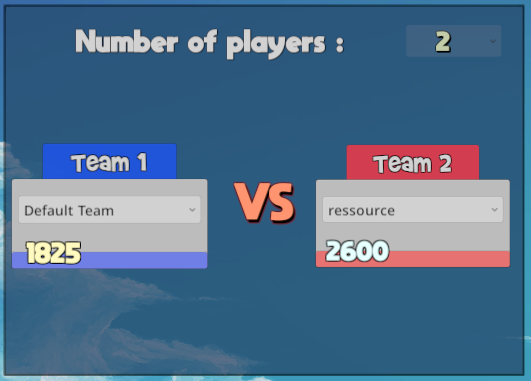
\includegraphics[scale=0.7]{DATA/Elo.png}
\captionof{figure} {Affichage des points}
\end{center}
\paragraph{}

% Ressource Race
\newpage
\section{Nouvelle condition de victoire}
A la fin du projet , après avoir intégré la gestion de la fin du jeu, M. Ferber nous a donné l’idée de mettre en place un second mode de jeu pour montrer les possibilités de généricité du projet. Le temps étant assez court, l’idée de mettre en place un mode de jeu entier était impossible , et nous avons mis en place une condition de victoire différente, mais toujours basée sur le mode de jeu WarBot.
\paragraph{}
Reprenant l’idée d’un mode réfléchi par l’équipe Game Design, la possibilité de passer en “Course aux ressources” a été rajoutée dans les paramètres. Si ce mode est sélectionné , l’utilisateur va pouvoir définir un temps limité en secondes avant l’arrêt de la partie, ainsi qu’une limite de ressource à atteindre. Le jeu s’arrête si le temps imparti est atteint, ou si l’une des équipes à atteint le nombre de ressources spécifié dans l’inventaire de leur base. Dans le cas où le temps est atteint, c’est l’équipe ayant le plus de ressources dans sa base qui a gagnée. 

\paragraph{}
\begin{center}
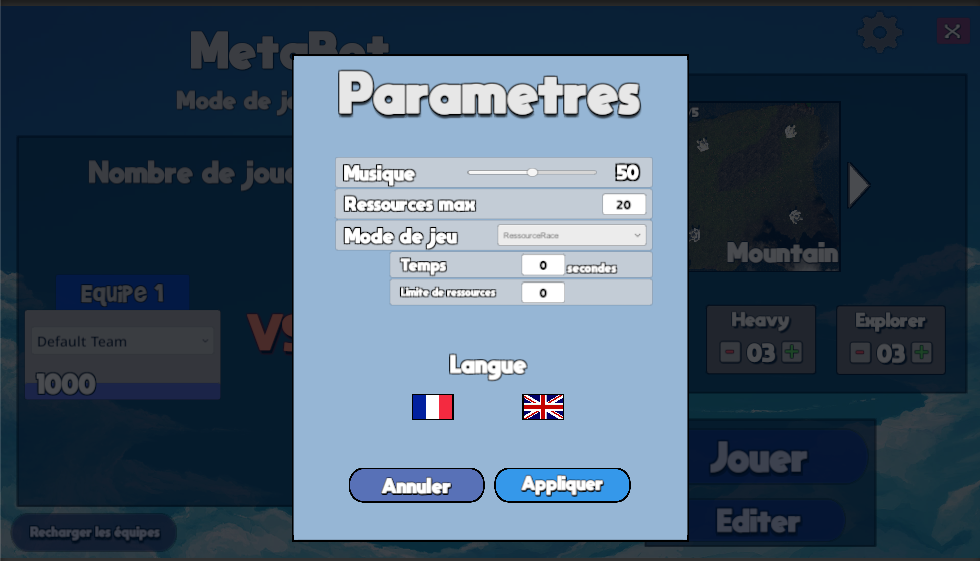
\includegraphics[scale=0.5]{DATA/param.png}
\captionof{figure} {Écran après l’animation}
\end{center}
\paragraph{}


Le but était de mettre en place un mode rapide mais qui justifierait le fait de pouvoir refaire des équipes adaptées à ce mode, au lieu d’utiliser uniquement les équipes de base qui ont été faites pour WarBot.

Nous avons ainsi pu rajouter une entrée dans les tableaux de fins du jeu, qui au lieu de vérifier le nombre de bases différentes toujours sur le terrain, va vérifier d’un côté dans chacune des bases du jeu si l’une d’entre elles a atteint la limite de ressource que l’on a données, et on va ensuite vérifier sur le Timer de jeu ,qui était déjà présent sur la carte par l’équipe Moteur, si la limite de temps est atteinte. Dans ce cas la on va déclencher la fin du jeu.
Il a été nécessaire de traiter un cas d’égalité dans ce mode-ci, puisque si aucune des équipes n’est capable de ramasser des ressources avant la fin du jeu il ne faut pas donner une victoire aléatoirement. 

La gestion de l’égalité se fait via un boolean, qui passe à vrai tant que l’on rencontre des bases qui ont le même nombre de ressources que la base considérée comme gagnante. 
Lors de l’affichage de l’animation , on va afficher le terme “Égalité” à la place d’une équipe gagnante, et surtout il ne faudra surtout pas faire l’appel de changements de stats des équipes.
\paragraph{}
\begin{center}
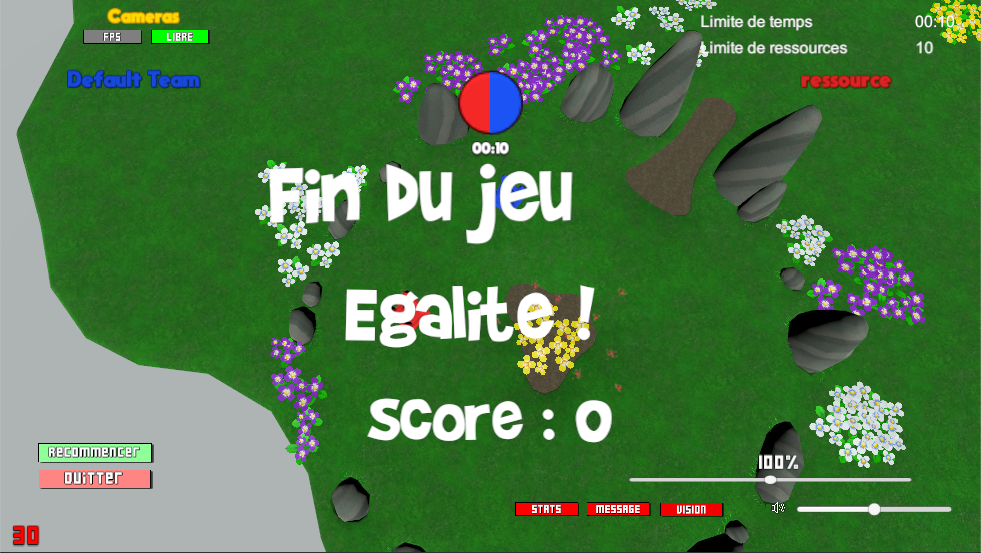
\includegraphics[scale=0.5]{DATA/egalite.png}
\captionof{figure} {Écran d’égalité}
\end{center}
\paragraph{}

\section{Début de la création d’une nouvelle carte}

Souhaitant s’essayer à la création d’une nouvelle carte, et suivant la création du mode de jeu des ressources, nous avons réfléchi à l’ajout d’une carte dans le jeu. 
Le temps étant trop court, et ayant d’autres priorités, la carte n’a pas été terminée, et ainsi l’équipe qui récupèrera le projet sera libre de pouvoir l’adapter comme bon leur semble.
\paragraph{}

Même si le but était la découverte de Unity sur la création de scène, nous avons cherché un moyen de rendre cette carte unique et ayant un intérêt. 
Avec une grande aide de l’équipe Game Design nous avons trouvé une configuration de carte équilibrée et utile. 

%Schéma carte ressources

Les bases ont été écartés aux 4 points cardinaux afin de les éloigner et limiter les combats. L’action est déplacée dans la zone centrale, où les ressources apparaissent et se retrouvent à même distance des 4 bases, les agents vont se déplacer en majorité. \newline
L’organisation des murs autour de chaque base rend plus difficile l’accès aux bases adversaires à cause des collisions qui vont renvoyer les agents dans une autre direction.

Bien sûr une équipe oubliant les ressources va tomber sur la base adverse si elle est située en face de soi, mais il n’est pas sûr que cette technique soit si rentable dans le mode Course aux ressources.

Un thème de carte qui plaît beaucoup et qui n’avait pas encore été exploré dans les 5 cartes du jeu est l’espace. 
Une idée était de représenter la carte comme un HUB central de vaisseau spatial, ce qui collait bien à la forme qu’on lui donnait.
\paragraph{}
Il a fallu trouver des textures de murs et de sol en rapport avec le thème, et nous avons pu apprendre le fonctionnement des “Skybox” dans Unity.
La skybox d’une scène un ensemble de 6 images correspondant à l’intérieur d’un cube (respectivement haut, bas , gauche, droit, arrière, avant) qui va être rendu par le jeu en après de tout le reste (donc en arrière-plan) , pour ne pas avoir un fond gris peu agréable pour l’utilisateur.
La skybox utilisée dans cette carte est tout simplement un fond noir, avec des étoiles pixélisées réparties.

Cette skybox a été générée par l’outil “Spacescape”, qui génère des skybox par couches, en générant des étoiles plus ou moins grosses.

\paragraph{}
\begin{center}
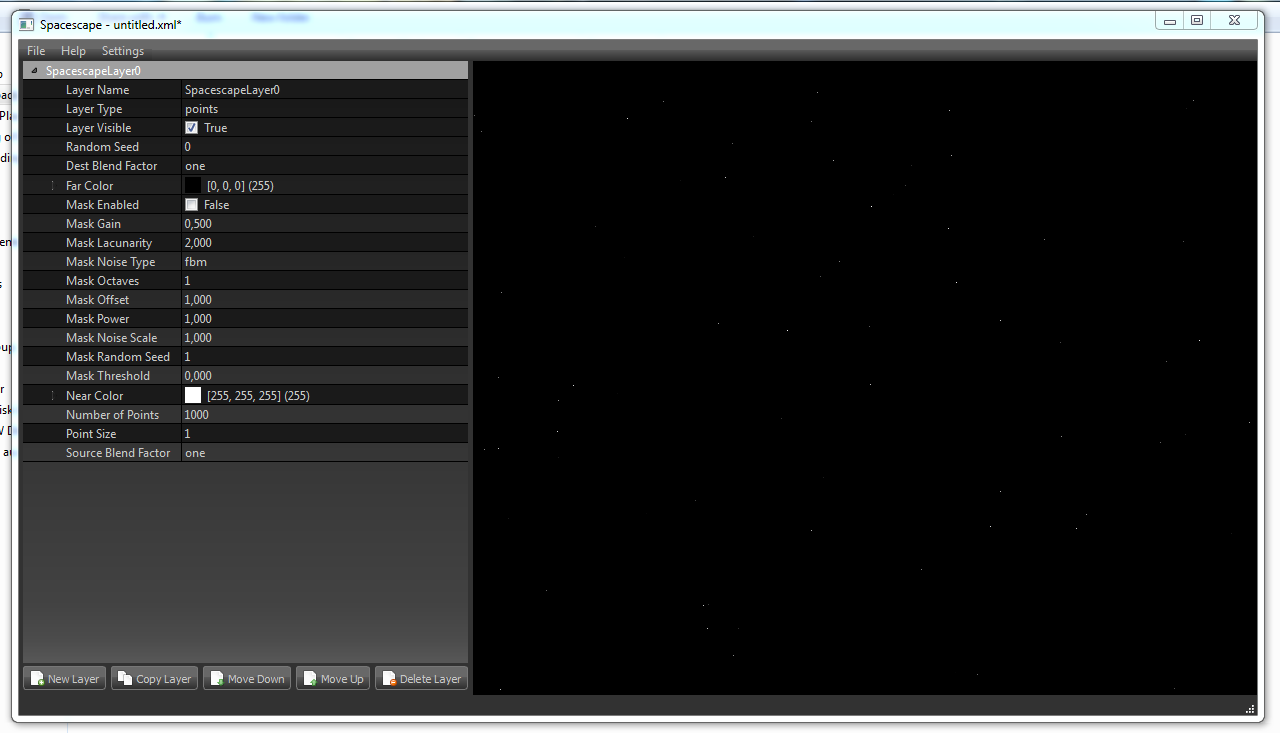
\includegraphics[scale=0.5]{DATA/spacescape.png}
\captionof{figure} {Outil Spacescape pour générer une skybox}
\end{center}
\paragraph{}

La carte a d'abord été mise en place sous forme de rectangle, pour bien comprendre le fonctionnement de Unity. Il  n’a pas été malheureusement possible de finir et de modifier la forme pour s’adapter au schéma, la carte est donc restée dans les fichiers du projet tel quelle.

Voici une image de l’état de la carte : 

\paragraph{}
\begin{center}
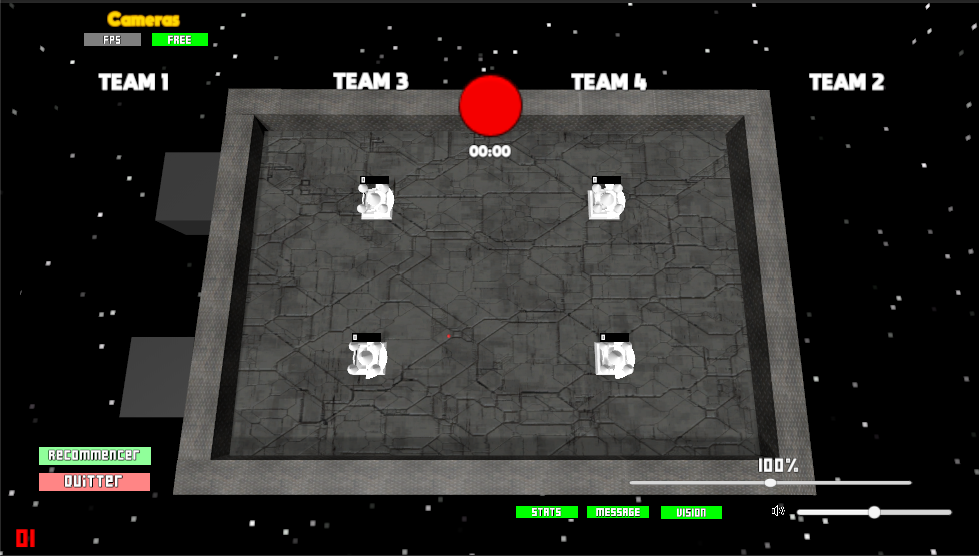
\includegraphics[scale=0.5]{DATA/space.png}
\captionof{figure} {Etat actuel de la carte}
\end{center}
\paragraph{}

La carte est présente dans la liste des cartes disponibles pour le jeu pour la démonstration, mais elle n’est qu’au stade présenté sur la capture d’écran ci dessus. Il faudra la retravailler pour qu’elle corresponde au schéma imaginé initialement.

\newpage
\chapter{Partie "Game Design"}
\section{Expérience utilisateur}
\subsection{Ancienne version de Warbot}
\paragraph{}
    Les premières semaines de ce projet ont étées l’occasion pour toute l’équipe de se familiariser avec la version de WarBot qui fut créée par les étudiants de l’année précédente. Nous avons donc immédiatement essayé de créer des équipes pour tenter d’apprivoiser son éditeur de comportement.
\paragraph{}
\begin{adjustwidth}{-2.5em}{}
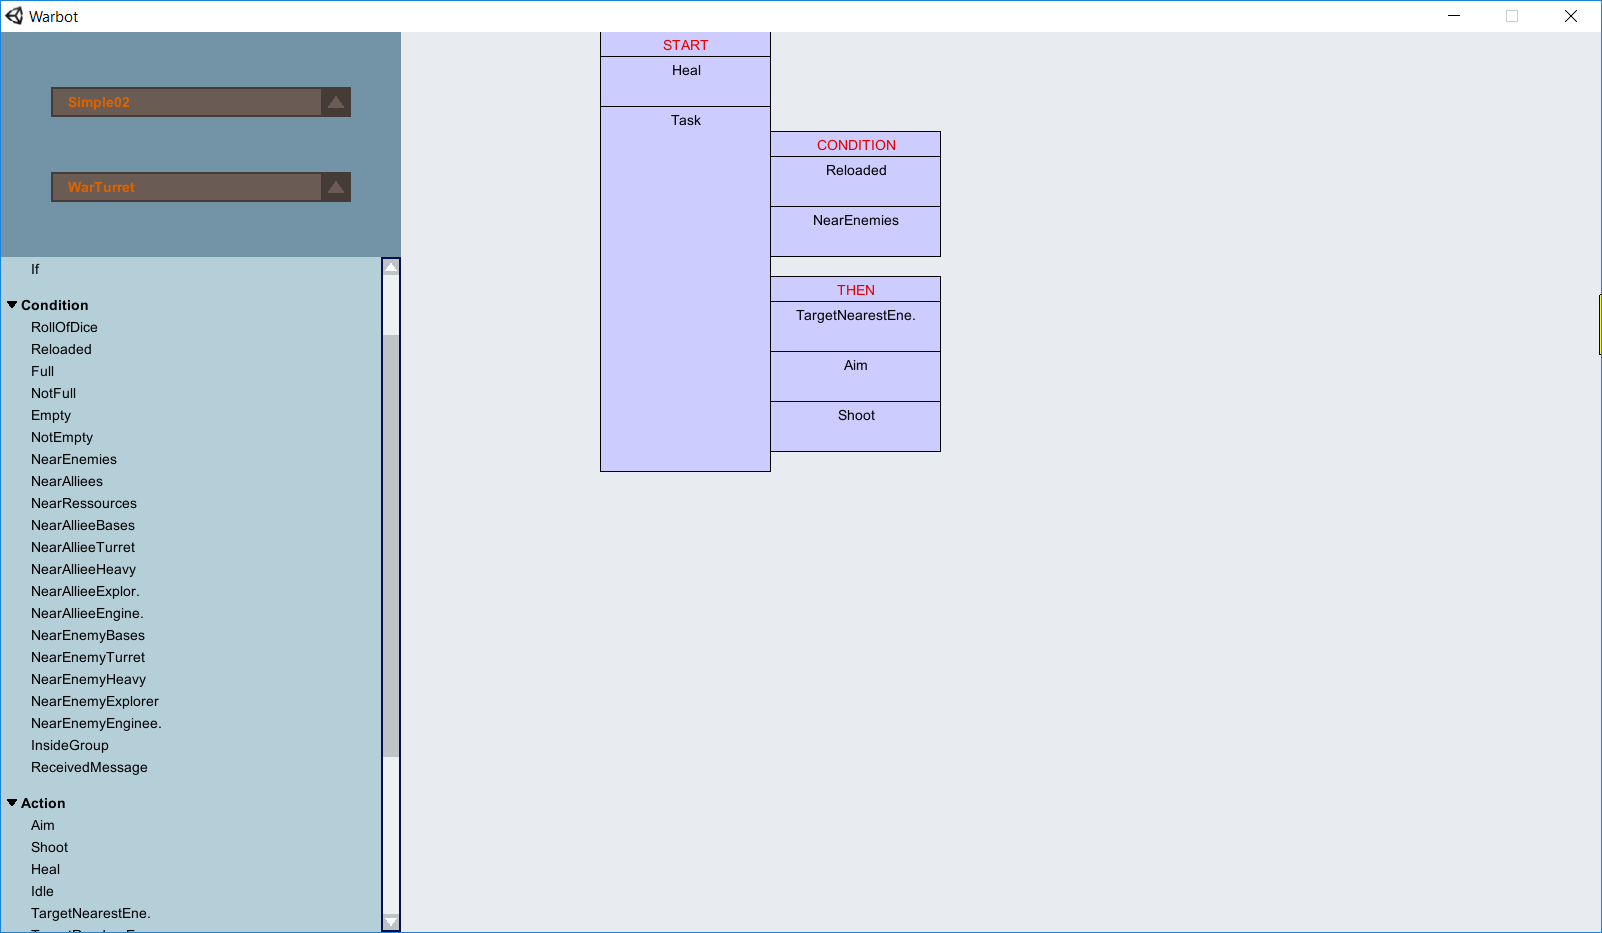
\includegraphics[scale=0.4]{DATA/oldEditor.png}
\captionof{figure} {Aperçu de l'ancien éditeur}
\end{adjustwidth}
\paragraph{}
    Nous nous sommes très vite rendu compte de plusieurs problèmes d’ergonomie qui rendait la création d’équipe difficile.
Tout d’abord, pour placer un bloc, il fallait :
\begin{itemize}
\item Cliquer sur le nom d’une primitive dans le menu de gauche
\item Maintenir le clic de la souris et déplacer le pointeur de la souris sur un bloc déjà placé
\item La primitive est ensuite placée en-dessous du bloc où se trouve le pointeur de la souris
\end{itemize}
Si cela semble simple sur le papier, en pratique c’est une tout autre histoire car le moindre faux mouvement positionnait le bloc au mauvais endroit ou le faisait disparaître.
En effet, si le curseur de la souris ne se trouvait sur aucun bloc au moment où on relâchait le clic, le bloc était tout simplement supprimé. \newline
Dans le cas où l’on avait mal positionné le bloc il fallait alors le déplacer. Cependant, cliquer sur un bloc déjà existant pour le bouger entraînait également le déplacement des blocs situés en-dessous de celui dont nous voulions modifier la position. Il fallait donc, dans un premier temps, sélectionner les blocs en-dessous de la primitive mal placée pour les positionner au-dessus de cette dernière pour pouvoir déplacer la primitive mal placée sans modifier le reste du comportement.
\paragraph{}
    Supprimer un bloc s’il n’est attaché à aucun autre bloc semble être une bonne idée car cette technique permet de ne pas avoir trop de blocs inutiles qui traînent dans l’interface. Seulement, un simple clic sur une primitive supprimait cette dernière ainsi que toutes celles placées en dessous de la primitive supprimée. Ceci s’explique par le fait que lors du clic sur une primitive, l’éditeur estime que nous somme en train de la déplacer. Or, comme on relâche la souris sans la bouger cette dernière est déplacé à un endroit où il n’y a aucun bloc entraînant ainsi la suppression des primitives. \newline
Ce problème était particulièrement dérangeant lorsque l’on souhaitait utiliser WarBot avec un pavé tactile car une simple pression sur ce dernier est compté comme un clic. Il n’était donc pas rare de supprimer une grosse partie de notre comportement en voulant repositionner son doigt sur le pavé tactile.
\paragraph{}
    A ceci s’ajoute l’absence de certaines fonctionnalités comme la possibilité d’annuler une modification ou de choisir quand sauvegarder le fichier, ce qui implique que chaque erreur était sauvegardée et la seule manière de la corriger était de replacer de nouveaux blocs pour revenir au comportement voulu.
\paragraph{}
    Cette version de WarBot possédait plusieurs types de primitives : les primitives de contrôle if et task, les conditions et les actions. Parmis les actions, certaines terminaient le tour de l’unité (tirer, bouger, se soigner…) alors que d’autres permettaient à l’unité de continuer son tour (Rejoindre un groupe, changer l’orientation de l’unité…). Il était difficile de savoir lesquelles terminaient le tour ou non car il n’y avait aucune différence visuelle entre ces deux types de primitives. Le seul moyen de savoir si une primitive permettait de continuer son tour était donc de passer sa souris sur le nom d’une primitive dans le menu à gauche pour avoir une description de la primitive dans laquelle il était précisé si cette action terminait le tour de l’unité. Dans le cas où l’action n’était pas terminale, aucune précision n’était rajoutée.
\paragraph{}
\begin{center}
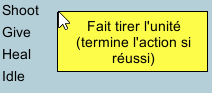
\includegraphics[scale=1]{DATA/terminale1.png}
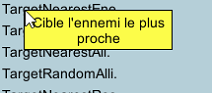
\includegraphics[scale=1]{DATA/terminale2.png}
\captionof{figure} {Comparaison descriptions}
\end{center}
\paragraph{}
    Un dernier problème d’ergonomie important est l’emplacement des boutons dans cet éditeur. En effet, il était possible de revenir au menu principal, de créer une nouvelle partie, de quitter le jeu et de créer une nouvelle équipe depuis l’éditeur. Cependant, les boutons qui permettaient ces actions étaient cachés dans le menu pause de l’éditeur. Le simple fait de pouvoir mettre en pause un écran qui n’en a pas besoin est déjà suffisamment contre-intuitive pour privilégier le fait de placer des boutons directement dans l’interface de l’éditeur plutôt que dans un menu accessible uniquement via la pression de la touche échap du clavier.
\paragraph{}
\begin{center}
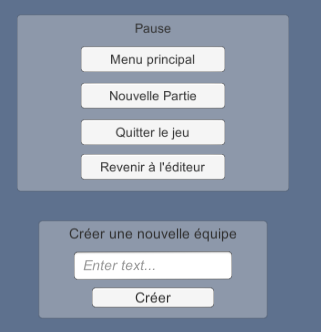
\includegraphics[scale=1]{DATA/oldPause.png}
\captionof{figure} {Fichier configuration}
\end{center}
\paragraph{}

\subsection{Création d’équipe sous la version actuelle}

\paragraph{}
La création d’équipe sous la nouvelle version de WarBot était un mélange de recherche de bugs et d’expérience utilisateur.
\paragraph{}
Pour créer une équipe nous partions d’une stratégie générale et nous développions les comportement à partir de cette idée. N’ayant pas encore la possibilité d’utiliser des groupes, les stratégies se limitaient souvent au choix entre une équipe défensive ou offensive.
\paragraph{}
Au vu de notre expérience, il y a une seule chose qui sépare ces deux genres d’équipes : l’ordre dans lequel on veut gérer les actions. Une équipe défensive va préférer mettre ses primitives pour se soigner au plus haut de sa hiérarchie pour que ce soit une action prioritaire, assurant la survie alors qu’une équipe offensive va préférer placer les actions de tirs et de rechargement avant les soins pour s’assurer d’effectuer des dégâts plus souvents. 
\paragraph{}
De manière générale,il y a quelques astuces importantes à prendre en compte pour optimiser le comportement d’une équipe. La première est de placer toutes les actions qui ne terminent pas le tour d’une unité comme les envois de message tout en haut de la hiérarchie pour s’assurer que ces actions soit effectués. On fait ensuite suivre les actions qui ont le moins de chances de se produire qui s’avèrent être les actions qui se font alors que l’unité est immobile (tirer, ramasser une ressource…) en les plaçant dans un ordre en particulier suivant la stratégie d’équipe que l’on souhaite appliquer. \newline
La deuxième est de préférer le système de création d’unité à l’aide de la vie car ce procédé permet de créer des unités dès le début de partie alors qu’une équipe qui crée des unités à partir des ressources devra attendre beaucoup plus longtemps avant de voir ses premières unités se former. Les ressources ramenées à la base sert alors à la soigner, ce qui permet de créer de nouvelles unités. L’avantage numérique étant très important dans le mode de jeu WarBot, il vaut mieux s’assurer de posséder beaucoup d’unités dès le départ si nous ne voulons pas nous mettre dans une situation dans laquelle il est presque impossible de reprendre l’avantage. L’inconvénient de cette technique est le fait de ne pas avoir beaucoup de vie mais l’avantage numérique nous semble beaucoup trop important pour arriver à former une équipe efficace qui préfère utiliser les ressources pour créer ses agents. \newline
Dernièrement, il vaut mieux respecter ce genre de comportement pour les déplacements :
\begin{lstlisting}[frame=single]
if(blocked) {
  heading random
  move
}
#Tout mouvement qui demande de se diriger vers quelque chose (base, message...)
if( ){
  move
}
\end{lstlisting}
De cette manière, le fait de se débloquer est prioritaire à tout déplacement. Ce qui permet de ne pas rester bloqué dans un obstacle.
\paragraph{}
  Lors de la création des équipes, nous avons pu apprécier les améliorations ergonomiques par rapport à l’ancienne version de WarBot. Le code est bien plus facile à lire grâce au code couleur qui différencie bien les différents types de blocs. De plus, le système de suppression de blocs a été changé : il faut maintenant faire un clic droit sur un bloc. Cette méthode permet de placer des blocs sans les rattacher aux blocs du comportement ce qui rend le déplacement de primitives plus simples et agréables. \newline
L’ajout d’un système de grille est également très agréable car les blocs sont naturellement attirés les un les autres ce qui permet de ne pas avoir besoin d’être précis lorsque que l’on place des blocs. \newline
Il est très facile de comprendre si nos blocs sont pris en compte dans le comportement grâce au système de coloralisation des pièces qui sont grisées si elles ne sont pas prises en compte et colorées si la primitive fait parti du comportement. \newline  
L’ajout de boutons de sauvegarde, de retour arrière et restauration rende également la partie conception bien plus agréable car il est possible de corriger ses erreurs bien plus simplement qu’avec la version de l’éditeur développé l’année dernière.\newline
La seule chose qui nous dérange encore sur la version actuelle est l’impossibilité d’utiliser la molette de la souris pour agir sur la partie de la fenêtre où l’on construit le comportement d’une unité ce qui demande de déplacer l’ascenseur avec sa souris, chose qui nous éloigne de l’endroit où se situe les primitives du comportement. Comme on utilise cet ascenseur pour pouvoir déplacer les blocs, il est dommage de devoir s’en éloigner avant de pouvoir effectuer le déplacement.\newline
La partie propriétés, bien qu’elle demande à être revu graphiquement fait son travail et permet de se donner une idée de l’intérêt de chaque unité qui permettra aux nouveaux joueurs de rapidement saisir les atouts et les faiblesses de chaques unités. Chose qui leur permettra de concevoir plus rapidement des équipes qui exploitent toutes les unités de manière optimale.
\paragraph{}
\begin{adjustwidth}{-5.5em}{-5.5em}
\begin{center}
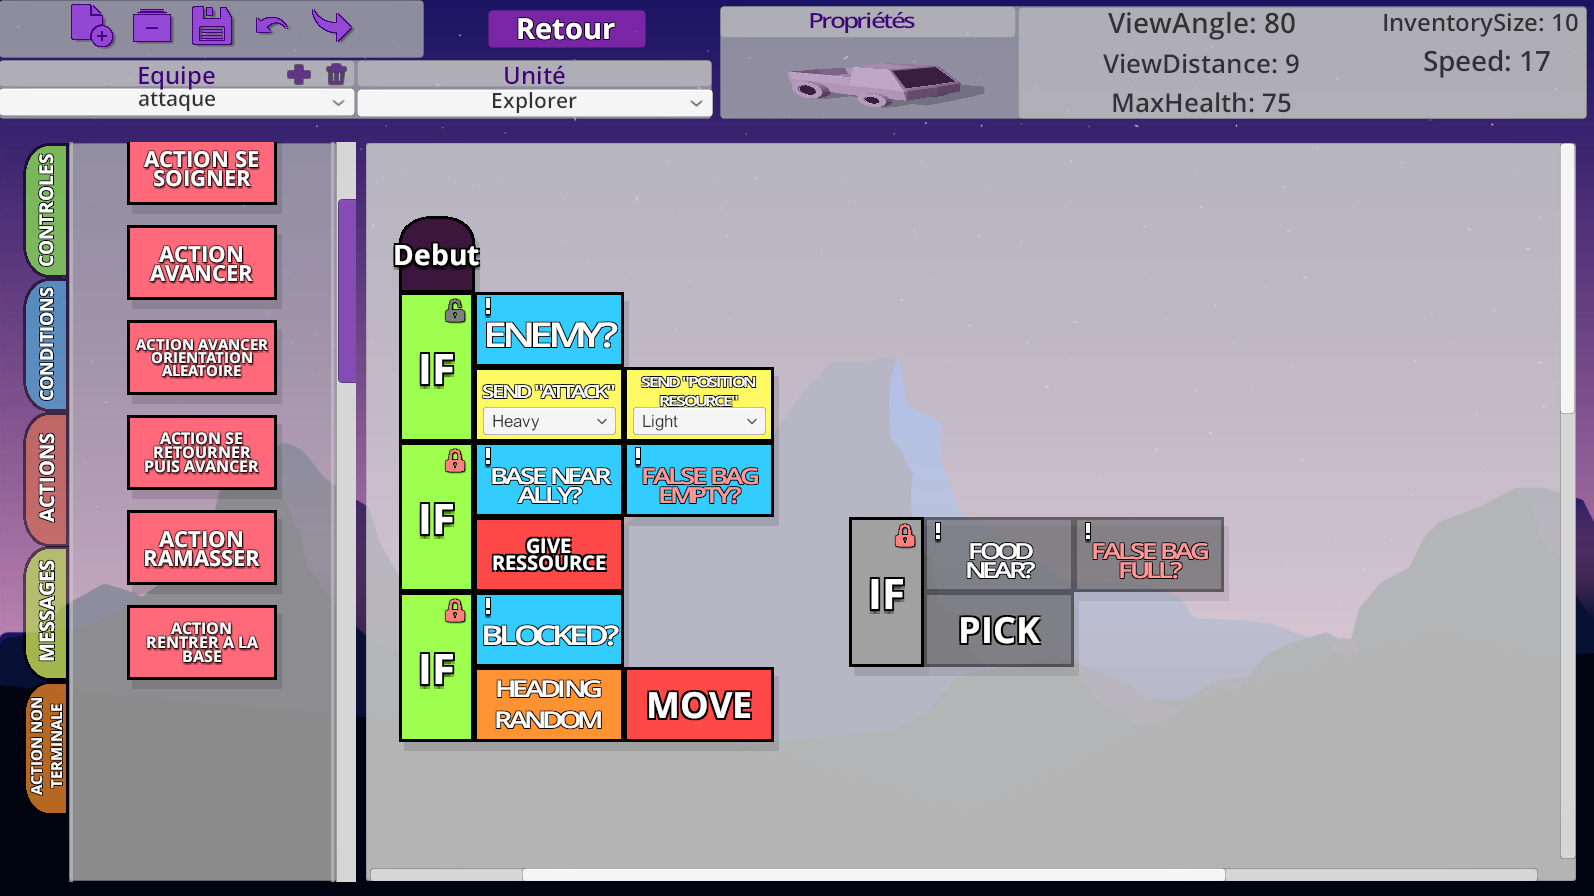
\includegraphics[scale=0.35]{DATA/editeurNew.png}
\captionof{figure} {Aperçu du nouvel éditeur}
\end{center}
\end{adjustwidth}
\paragraph{}

Malheureusement, les groupes ne sont plus présents dans cette version, ce qui rend le nombre d’option bien plus limité.\newline
La disparition des unités WarEngineer et WarTurret rend également le jeu moins complet. Les tourelles étant des outils très intéressant pour les stratégie défensive, ces équipes sont bien moins fortes que dans la version faite l’année dernière.
\section{Test logiciel}
\subsection{Procédé}
\paragraph{}

Même si nous arrivions à trouver des bugs lors d’une utilisation normale du logiciel, ce n’est pas suffisant pour trouver tous les bugs présents sous WarBot. \newline
En effet, dans le domaine de tests logiciels il existe plusieurs familles de tests. Il est important de préciser que nous avons effectué les tests en boîte noire, c’est-à-dire en ayant très peu, voire pas du tout, de connaissance du code du logiciel. La première est le test des nouvelles fonctionnalités dont le but est de se focaliser sur les nouveautés de la version pour vérifier qu’elles marchent bien. Pour effectuer ces tests, nous avons créé des équipes très simples n’utilisant presque qu’une seule primitive à savoir celle que l’on voulait tester. Nous lancions ensuite une partie et observions le comportement des unités pour déterminer si les ajouts étaient bien opérationnelles.
\paragraph{}
  Une fois les tests des nouvelles fonctionnalités terminés, nous faisions des tests combinatoires dont le but était de vérifier que de mêler plusieurs primitives dans un même comportement ne posait pas de problème. Pour cela, nous complexifiions les équipes créés pour tester des primitives à part en rajoutant de nouvelles primitives dans leur comportement.
 \paragraph{}
  Une autre famille de test très importante est la famille des tests de non régression. Le but de ces tests est de tester toutes les anciennes fonctionnalités pour vérifier si elles fonctionnent toujours de la même manière que dans la version précédente. Pour cela, nous lancions une partie avec des équipes créés lors des versions précédentes et nous vérifions que les agents n’avaient pas de comportement étranges ou non désirés.
\paragraph{}
  Lest derniers tests que nous avons effectués sont les tests aux limites. Ces tests consistaient à pousser WarBot dans ses retranchements en essayant des choses qui étaient susceptibles de ne pas avoir été pensé par les développeurs. Par exemple, nous avons essayé de créer des équipes dont le nom contenaient des caractère spéciaux, de lancer des parties avec énorméments d’unités, de constamment changer la vitesse en jeu...

\subsection{Organisation et communication}
\paragraph{}
  Une fois qu’un bug était trouvé, nous tentions de le reproduire plusieurs fois afin de comprendre comment le déclencher. Une fois que le déclenchement du bug était compris, nous l’ajoution à la liste de bugs.
\paragraph{}
  Cette liste étant un Google Document partagé, n’importe qui possédant le lien vers ce document étaient capable de le voir et de l’éditer. Le but était donc de centraliser tout le processus de communication des bugs : n’importe qui pouvait ajouter à la liste un bug qu’il avait découvert, indiquer la correction d'un bug ou la réapparition de certains bugs que l'on croyait corrigés.
\paragraph{}
  Ce document possède plusieurs tableaux : un pour les bugs non traités, un pour ceux qui sont réapparus après une correction, un pour les bugs patchés (non corrigé mais un compromis a été réalisé pour que ça ne pose plus de problème), un pour les bugs à vérifier et un dernier pour les bugs corrigés.
\paragraph{}
Il nous arrivait également de rajouter des liens vers des vidéos des bugs enregistrées lors de nos sessions de recherche de bugs ou bien des captures d’écrans, rendant ainsi plus explicite les problèmes qu’apportent le bug ou la manière de le réaliser.
\paragraph{}
Lorsqu’un bug était plus important, comme l’impossibilité de lancer une partie ou de créer un comportement, nous en informions directement l’équipe via notre serveur Discord qui permet d’effectuer des conversations instantanées avec tous les membres du groupe. Ces conversations peuvent être aussi bien textuelles que vocales. L’intérêt de passer directement par Discord était de provoquer une situation d’urgence où toute l’équipe était mise au courant du problème sans qu’ils aient besoin de passer sur le Google Document. 

\section{Game Design}

\subsection{Amélioration demandés}
\paragraph{}
  Deux semaines après le début du projet, il nous a été demandé de rédiger un document expliquant comment nous voulions voir langage évoluer. Nous avons donc commencé à imaginer comment améliorer le langage de l’éditeur de l’ancienne version.
\paragraph{}
  Tout d’abord, nous voulions introduire une nouvelle fonctionnalité : l’objectif. Au vu de la nature d’une architecture de subsomption qui est le concept sur lequel se base le comportement des agents de WarBot, il est très dur de réaliser des stratégie car la moindre réponse à un réflexe nous fait perdre notre trajectoire car l'orientation de l'unité est modifiée. \newline
L’objectif est donc un objet contenant simplement des coordonnées qui se conserve au fil des tours, contrairement à la cible. Il a été conçu notamment pour se diriger vers des messages. Le but est de conserver la position de l’émission d’un message pour pouvoir se diriger vers ce dernier à tout moment. \newline
Ainsi, il est possible de réagir à des réflexes sur un tour puis de modifier son orientation en direction de l’objectif pour reprendre le chemin vers ce dernier aux tours suivants. Cette fonctionnalité permet également de tirer vers une position en dehors de notre champ de vision, possibilité imposé par M. Ferber qui veut que les WarHeavy aient une distance de vue très faible pour que les autres unités soient obligés de les guider.
\newpage
\paragraph{}
  Le gros problème de l’ancien éditeur venait de son ergonomie. Pour l’améliorer, nous avons proposé un système de code couleur et de forme de pièces, réalisé à l’aide d'un logiciel de traitement d'image pour servir de référence à l’équipe interface :

\paragraph{}
\begin{center}
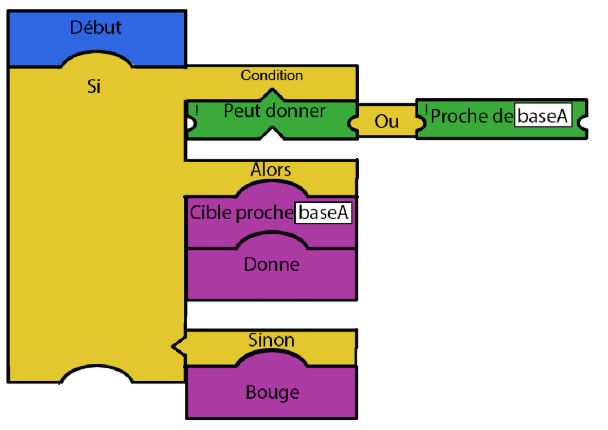
\includegraphics[scale=0.7]{DATA/propLangage.png}
\captionof{figure} {Aperçu d'un comportement avec la refonte proposée}
\end{center}
\paragraph{}

Ici, toutes les structures de conditions sont en jaunes, toutes les actions en violettes et toutes les conditions en vertes. \newline
Le système de forme de bloc permettait également de comprendre immédiatement où on pouvait placer des blocs. Les actions peuvent être positionné sous les blocs possédant un creux ovale alors que les conditions ne peuvent être positionnées qu’en-dessous des blocs possédant des creux triangulaires.
Les actions terminales ne possèdent pas de creux en bas du bloc pour exprimer le fait qu’il est impossible de positionner d’autres blocs à leur suite. \newline
Les conditions ont également des “!” en haut à gauche de leur bloc. Un clic sur ce dernier changeait la couleur du bloc exprimant ainsi que nous ne testions plus si la condition est vraie mais si la condition est fausse.

\paragraph{}
\begin{center}

\includegraphics[scale=0.8]{DATA/negation.png}
\captionof{figure} {Condition normale et sa négation}
\end{center}
\paragraph{}

  Au vu de notre expérience utilisateur, nous avons également voulu l’ajout de plusieurs primitives. Les premières étant un nouveau groupe de blocs : les variables. Voici la liste de celle que nous voulions rajouter à WarBot :
  \begin{itemize}
\item Vie actuelle qui donne la vie restante de l’unité
\item Ressource actuelle qui donne le nombre de ressources dans le sac de l’unité.
\item Porté de tir qui donne la porté de l’arme de l’unité
\item Distance objectif qui donne la distance entre l’unité actuelle et son objectif
\item Distance cible qui donne la distance entre l’unité actuelle et sa cible
\item Nombre membre qui donne le nombre de membre au sein d’un groupe précisé en paramètre
\item Lancé de dé qui retourne un nombre aléatoire entre 1 et la borne maximale passée en paramètre
\item Constante qui permet d’écrire n’importe quelle donnée
\end{itemize}
\paragraph{}
  Ces variables servaient surtout à utiliser les opérateurs de comparaison ( inférieur, supérieur, égale) qui est l’une des conditions que nous voulions ajouter : 

\paragraph{}
\begin{adjustwidth}{-6em}{}
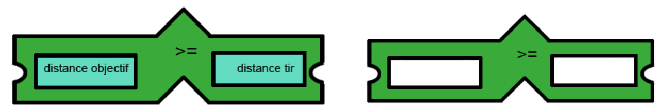
\includegraphics[scale=1]{DATA/comparaison.png}
\captionof{figure} {Condition de comparaison}
\end{adjustwidth}
\paragraph{}

Les blocs bleus cyans représentent les variables qui sont de simples rectangles pour exprimer le fait qu’on ne peux les positionner qu’ici. \newline
Les autres conditions que nous voulions ajouter sont :
\begin{itemize}
\item A un objectif qui retourne true si l’unité à un objectif
\item Niveau de vie qui prend un double entre 0 et 1 comme paramètre et qui renvoie true si 
\[
vie Atuelle De L’unite > vie Maximale De L'unite * parametre
\]
\item Niveau de ressource qui prend un double entre 0 et 1 et qui renvoie true si 
\[
nombre Ressource De L'unite > taille Inventaire De L'unite * parametre
\]
\end{itemize}
\paragraph{}
  Pour les derniers ajouts de primitives, il nous fallait deux primitives pour gérer la notion d’objectif :
  \begin{itemize}
\item Définir objectif qui affecte à cette variable un objet possédant les coordonnées de la cible actuelle
\item Supprimer objectif qui permet de libérer l’unité de son objectif.
\end{itemize}
\paragraph{}

  Dernièrement, nous avons listé quelles primitives n’était pas intéressantes et celles qu’il fallait modifier :
\begin{itemize}
\item Task car c’est une primitive qui ne se différencie pas assez de la primitive if pour être conservée
\item Not full et not empty car la possibilité d’exprimer la négation d’une condition les rends redondantes avec les négations de full et empty
\item SelectUnite ne servait qu’à créer des unités. En effet, il fallait sélectionner le type d’unité que nous voulions créer puis appeler la primitive create unit. Le fait d’appeler simplement create unit et de sélectionner l’unité voulu via un menu déroulant était donc suffisant.
\paragraph{}
\begin{center}
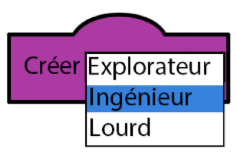
\includegraphics[scale=1]{DATA/deroulant.png}
\captionof{figure} {Le menu déroulant déroulé}
\end{center}
\paragraph{}
\item TargetNearest existait en plusieurs exemplaire (un pour chaque type d’unité, le tout multiplié par deux pour différencier les ennemis des alliés). Nous voulions les remplacer par une variable “Cible” que l’on aurait affecté via une primitive qui aurait eu un menu déroulant pour sélectionner ce qu’on voulait cibler (ennemi, allié, message, ressources…)
\item Near avait les mêmes problèmes que TargetNearest. Nous voulions donc utiliser une solution similaire en créant une primitive “proche de” ayant le même système de menu déroulant.
\end{itemize}
\newpage
\subsection{Game Document}
\paragraph{}
  L’un des deux buts majeurs de notre équipe lors de ce projet a été de créer de nouveaux modes de jeu, différent de WarBot.
\paragraph{}
  Il existe deux approches créatrices majeures en conception de jeu. L’approche bottom-up où l’on part d’un ou plusieurs éléments de gameplay auquel on tente d’appliquer un contexte est l'une d'entre elles. C’est par exemple le cas du jeu Splatoon de Nintendo qui n’était au départ qu’un prototype qui utilisait le gyroscope de la console Nintendo Wii U afin de repeindre un cube. A partir de cette idée principale d’autres éléments comme le fait de se déplacer dans sa peinture ont été rajouté puis il a été décidé du contexte et du scénario du jeu à la toute fin. \newline
L’autre approche est l’approche top-down dans laquelle on commence par déterminer le scénario ou une intention de jeu pour lesquels on crée des mécaniques qui s’inscrivent dans l’expérience voulue. C’est l’approche qui est choisi pour des jeux à licence comme les Batman Arkham où il faut créer des mécaniques qui s’appuient sur la personnalité de Batman et du monde décrit dans ses comics. D’autres jeux comme Journey partent d’une envie de créer une certaine expérience de jeu qui dans le cas présent était de créer un jeu social se basant sur le partage d’émotions. \newline
Nous avons choisi l’approche top-down car notre but dans la création de nouveau mode était de créer des modes se différenciant du mode WarBot. Il était donc plus logique de partir d’une intention de jeu précise suffisamment différente de ce qui est demandé dans le mode WarBot pour se détacher de ce dernier.
\paragraph{}

  Nous avons donc commencé à chercher des idées en ayant eu pour consigne de faire quelque chose de différent de WarBot sans trop s’en éloigner. Parmis ces idées, nous avons décidé de développer celles que nous trouvions les plus pertinentes à savoir un jeu en coopération basé sur la collecte de ressources, un simili RPG où les agents devaient accepter des quêtes de personnages non joueur et un jeu d’énigme. \newline
Au final, seulement l’idée du jeu de coopération a été accepté par le reste de l’équipe mais il a été jugé trop complexe et il nous a donc été demandé de retravailler ce mode. On nous a également demandé de travailler sur la conception d’un mode de jeu de capture de drapeau car implémenter un mode de jeu qui partage un grand nombre de primitives avec WarBot semblait bien plus faisable que la création d’un mode de coopération qui demandait de plus amples réflexions afin de le faire fonctionner sous le moteur de jeu développé cette année.
 \paragraph{}
 \newpage
  Après avoir sélectionné les idées à développer, nous avons commencé à penser la conception des modes. En partant de l’idée générale, nous avons définis quel genre d’objectifs nous voulions imposer aux joueurs pour rendre le mode intéressant. Par exemple, pour le mode de capture de drapeau, nous voulions obliger le joueur à créer une équipe capable de défendre une zone. \newline
Une fois cet objectif défini, nous réfléchissions aux problèmes éventuels que l’idée allait impliquer et nous ajoutions de nouvelles règles et mécaniques dans le but de diriger le mode de jeu dans la direction voulue. Toujours pour la capture de drapeau, nous avions peur que les parties soient trop passives car dans la version la plus courante de ce mode de jeu, chaque équipe possède un drapeau à défendre et doit en plus récupérer celui de l’adversaire. Nos craintes se basaient sur l'hypothèse que l’attaque serait moins intéressant que la défense, ce qui aurait entraîné de nombreuses parties interminables où aucune des deux équipes n’arrive à récupérer le drapeau adverse. Pour résoudre ce problème, il a été décidé qu’il n’y aurait qu’un seul drapeau n’appartenant à aucune équipe et que l’équipe qui le ramènerait à sa base remporterait le match.
\paragraph{}

  Une fois toutes les mécaniques définis nous passions à la rédaction du game document dans lequel nous expliquons les règles du mode (objectifs, interaction entre agents…), les éléments de jeu dont nous avons besoin, les intentions du mode et en quoi il se sépare de WarBot, une liste des primitives nécessaire pour ce mode ainsi qu’une ébauche de direction artistique qui sert de contexte pour justifier les éléments de gameplay.
\paragraph{}

  La grande difficulté de cette partie était le fait que le joueur n’intervient pas au cours de la partie : son seul but est de créer des comportements pour une équipe qui jouera toute seule. Ce problème devient double parce que nous n’étions pas particulièrement au courant des méthodes utilisées lors de conception d'un jeu ce qui nous a donc demandé à la fois d’apprendre la méthodologie et de l’adapter à un jeu où il n’y a pas de joueur. \newline
En effet le simple fait de ne plus prendre le joueur en compte dans l’équation enlève des principes fondamentaux de la conception de jeu comme la boucle de gameplay ou le game feel. 
Le principe de la boucle de gameplay est que  pour un objectif donné, il existe un challenge et une récompense qui doit être proportionnelle à la difficulté qui lui ai associé. Il existe des boucles de gameplay à plusieurs niveaux : micro, moyen et macro. Voici ce que des boucles de gameplay dans un RPG pourrait être.
\paragraph{}
\begin{figure}
\begin{adjustwidth}{-8em}{-7em}
\begin{subfigure}{.5\textwidth}
  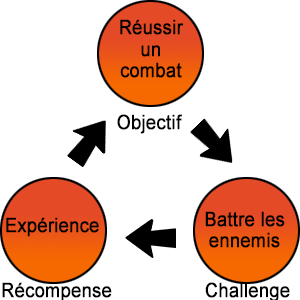
\includegraphics[scale=0.5]{DATA/boucleMicro.png}
  \caption{Boucle micro}
  \label{fig:sfig1}
\end{subfigure}%
\begin{subfigure}{.5\textwidth}
  \centering
  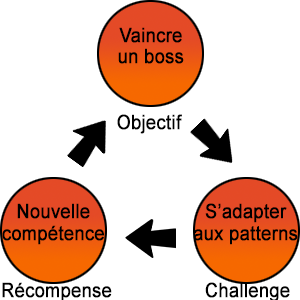
\includegraphics[scale=0.5]{DATA/boucleMoyene.png}
  \caption{Boucle moyenne}
  \label{fig:sfig2}
\end{subfigure}
\begin{subfigure}{.5\textwidth}
  \centering
  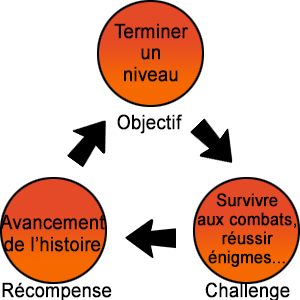
\includegraphics[scale=0.5]{DATA/boucleMacro.png}
  \caption{Boucle macro}
  \label{fig:sfig3}
\end{subfigure}
\caption{Boucle de gameplay d'un RPG}
\label{fig:fig}
\end{adjustwidth}
\end{figure}
\paragraph{}
\newpage
Seulement, avec WarBot, nous devons supprimer les boucles micro et moyenne pour ne conserver qu’une boucle macro :

\paragraph{}
\begin{center}
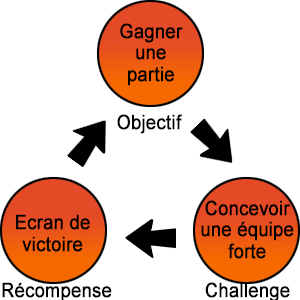
\includegraphics[scale=0.7]{DATA/macroWarBot.png}
\captionof{figure} {Boucle de gameplay de Warbot}
\end{center}
\paragraph{}

Normalement, nous devrions posséder des boucles moyennes elles mêmes composés de boucles micros au sein de la boucle macro pour stimuler l’intérêt du joueur au cours de la partie, chose impossible avec WarBot car même si l’on peut définir des objectifs au niveau moyen (défendre la base, lancer une attaque…) et micro (détruire une unité, créer une nouvelle unité…) il est impossible de créer du challenge au sein de la partie pour le joueur. Ce challenge est néanmoins présent lors de la conception d’une équipe mais comme il est impossible d’avoir une récompense directement après avoir surmonté le challenge car il faut lancer une partie pour obtenir cette récompense, l’effet de la résolution d’un objectif est amoindri. Le fait que le challenge soit toujours le même pour un objectif différent peut également entraîner l’ennui chez le joueur qui l’amènera à se désintéresser du jeu.
\paragraph{}


  Le game feel, quant à lui, est un concept défini par Steve Swink dans son livre Game Feel : A Game Designer’s Guide to Virtual Sensation. Ce concept explique que chaque jeu doit penser le contrôle de son personnage ainsi que les mécaniques de son jeu afin de servir une intention de jeu. Par exemple, un jeu de combat comme Street Fighter 5 va donner peu de contrôle aérien à ses personnages et faire en sorte que les coups des personnages soient suffisamment lent pour permettre aux joueurs de lire et punir ses adversaires. De même, les coups lents permettent de lier plus facilement les coups d’un combo ensemble car le jeu souhaite que les joueurs s’adaptent et réagissent à la phase de jeu actuel plutôt que de demander de bêtement appuyer sur des touches en espérants qu’il se passe quelque chose. Ces décisions amènent à un ressenti de lourdeur et de rigidité du gameplay qui dirigent l’expérience de jeu vers ce que les concepteurs ont prévus. \newline
A l’opposé, on retrouve des jeux comme Super Mario 64 où les concepteurs ont voulu donner une grande liberté de mouvement à Mario car le but des game designer est de s’assurer que le coeur du jeu, à savoir les mouvements, était suffisamment intéressant pour porter le jeu tout entier. Pendant les premiers mois de développement, ce jeu ne possédait d’ailleurs aucun niveaux car les concepteurs se sont assurés que les déplacements à eux seuls étaient amusants en laissant Mario sur un sol plat où le seul but était d’attraper un lapin, sans risque d’échec. Mario donne l’impression de flotter dans les airs, ce qui a été décidé afin que le joueur puisse facilement modifier sa direction en l’air pour atterrir sur les plateformes. \newline
Le problème avec WarBot est alors évident : le joueur ne contrôle pas ses unités ce qui implique qu’il est impossible de déterminer un game feel qui aurait pu nous servir pour déterminer quel genre de mécaniques et d’objectifs nous aurions pu implémenter si nous avions un game feel que nous souhaitions implémenter au jeu.
\newpage
\subsection{Design des cartes de jeu}
\paragraph{}
  Lors de la décision d’ajouter un mode de jeu où la condition de victoire était le nombre de ressources récoltées, nous avons conçu trois nouvelles cartes. Dans ces trois cartes, on retrouve une zone violette qui représente la zone où les ressources apparaîtront et des maisons de différentes couleurs représentant les positions des différentes bases.

\paragraph{}
\begin{center}
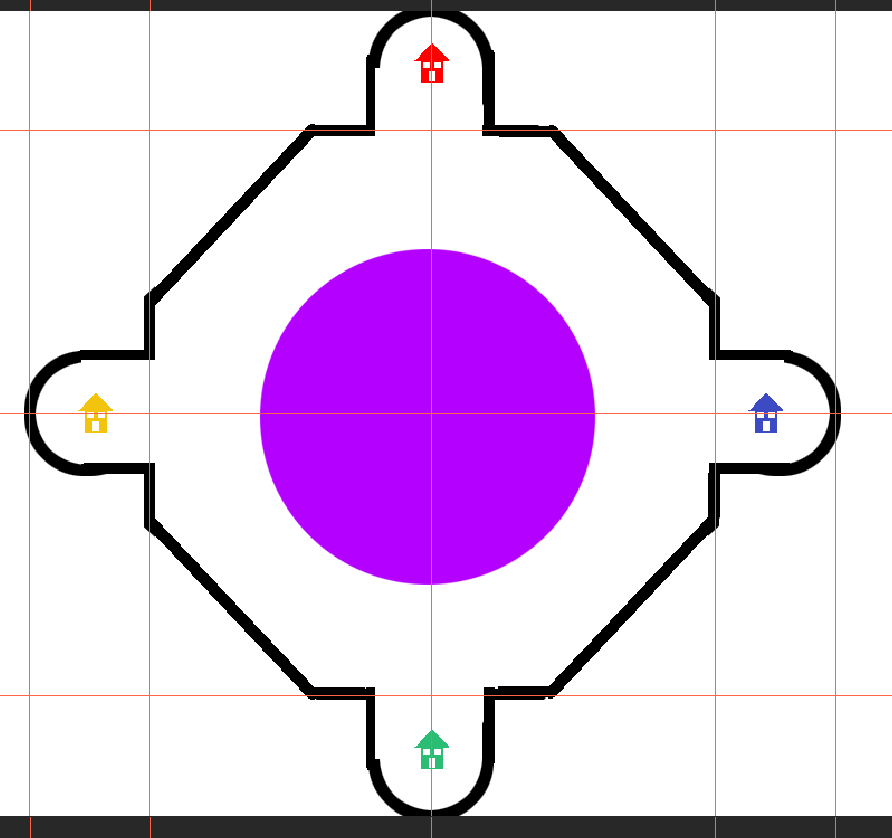
\includegraphics[scale=0.2]{DATA/carte+.png}
\captionof{figure} {Carte 1 mode ressource}
\end{center}
\paragraph{}

Cette carte est la carte la plus simple. Les bases sont dans des espaces clos assez difficile d’accès pour centraliser l’action dans une seule zone : le centre. La zone centrale est en forme d’octogone afin de limiter les zones où il n’y a rien d’intéressant toujours dans l’intention de focaliser l’attention des agents sur la zone d’apparition des ressources.
\newpage
\paragraph{}
\begin{center}
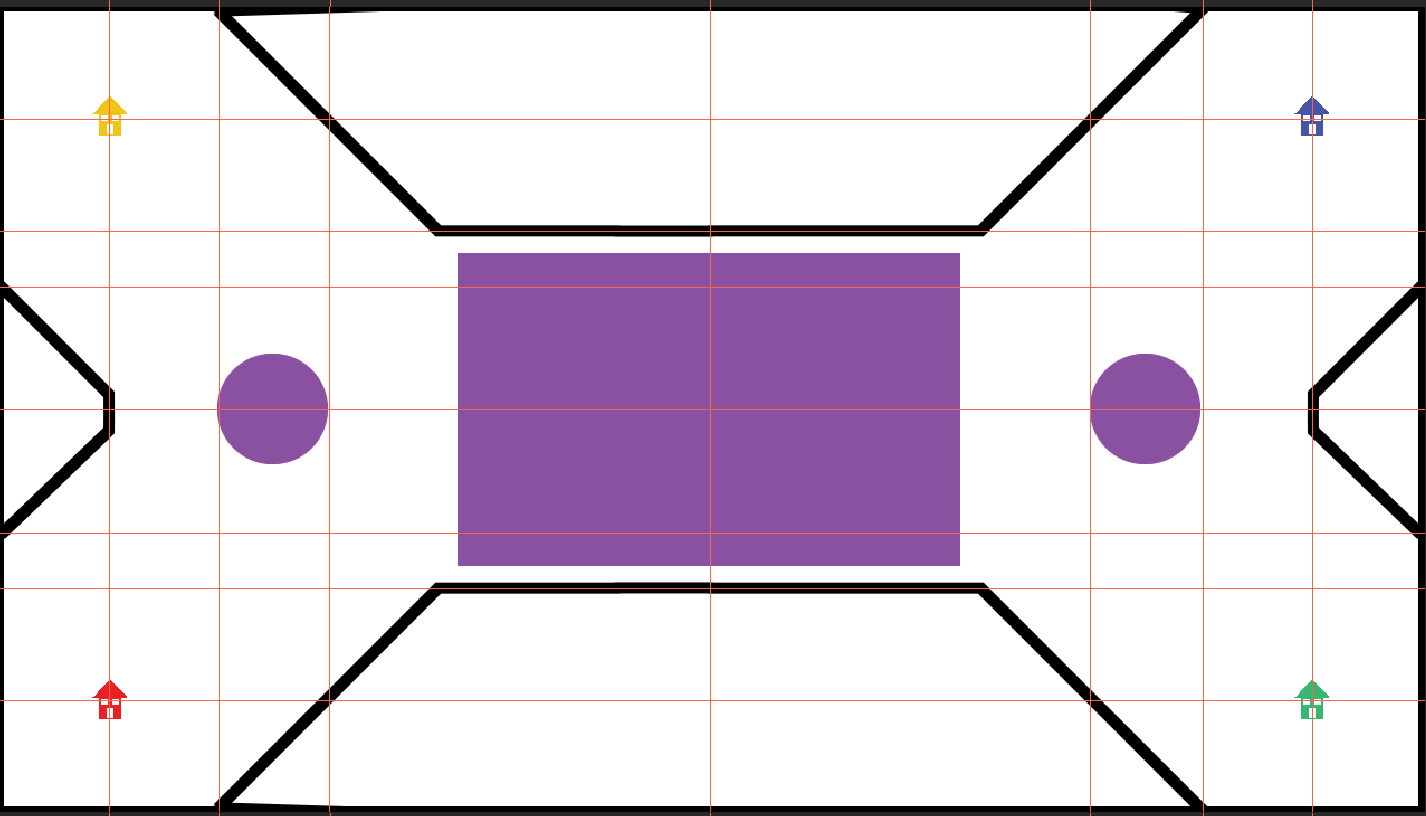
\includegraphics[scale=0.2]{DATA/carteX.png}
\captionof{figure} {Carte 2 mode ressource}
\end{center}
\paragraph{}

Ici, on tente de séparer les zones d’intérêt en ajoutant deux zones d’apparition de ressources séparés de la zone central pour provoquer des affrontements entre les deux équipes disposé sur le même côté de l’écran. Ces zones sont volontairement petite pour faire en sorte que les agents préfèrent aller dans la zone centrale qui serait bien plus abondante en ressource.

\paragraph{}
\begin{center}
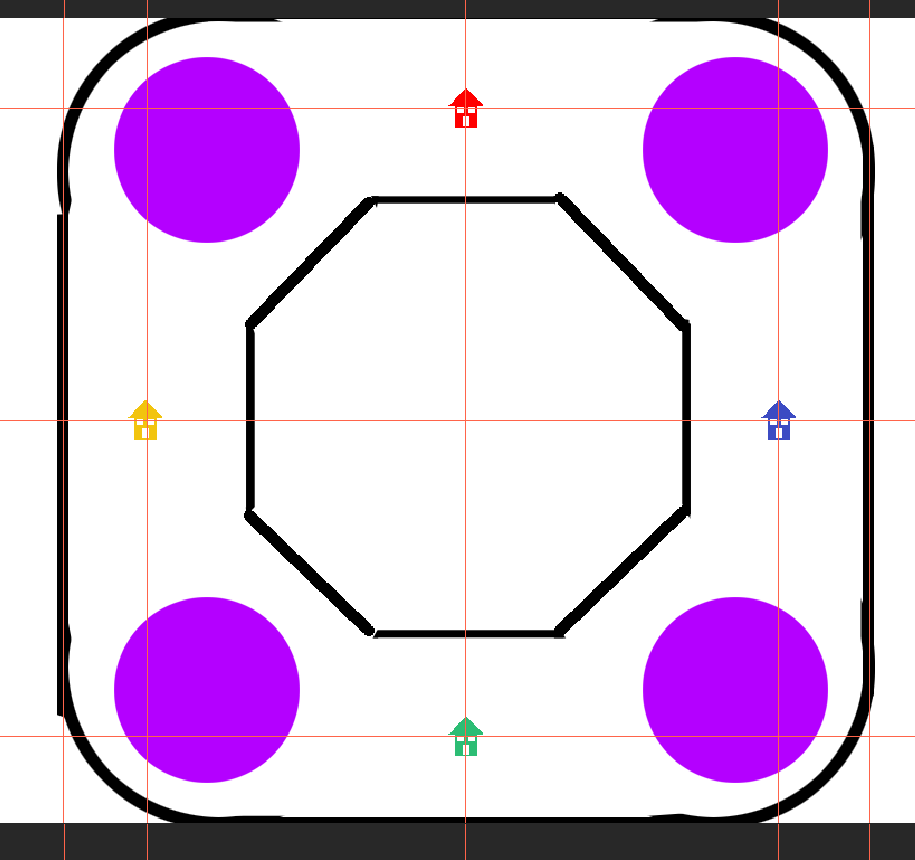
\includegraphics[scale=0.2]{DATA/carteO.png}
\captionof{figure} {Carte 3 mode ressource}
\end{center}
\paragraph{}

Pour cette dernière carte, le but était de séparer les affrontements dans plusieurs zones pour obliger les affrontements entre deux équipes pour trancher avec les autres cartes où les quatres équipes s'affrontent au même endroit, d’où la zone centrale inaccessible.

\paragraph{}
\begin{figure}
\begin{adjustwidth}{-8em}{-7em}
\begin{subfigure}{.5\textwidth}
  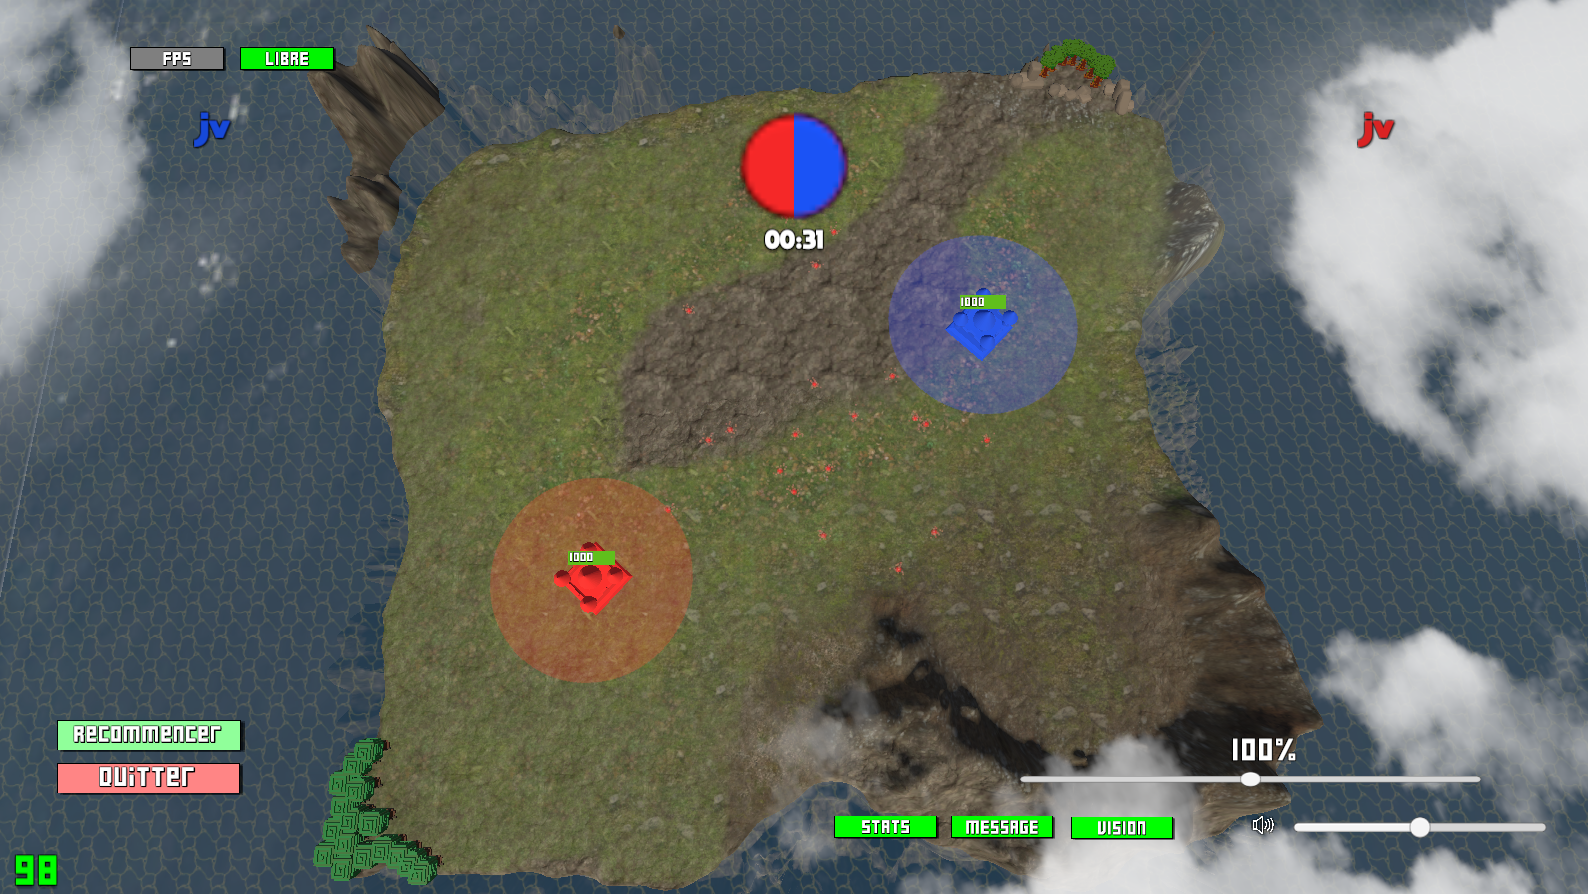
\includegraphics[scale=0.1]{DATA/montagne.png}
  \caption{Mountain}
  \label{fig:sfig1}
\end{subfigure}%
\begin{subfigure}{.5\textwidth}
  \centering
  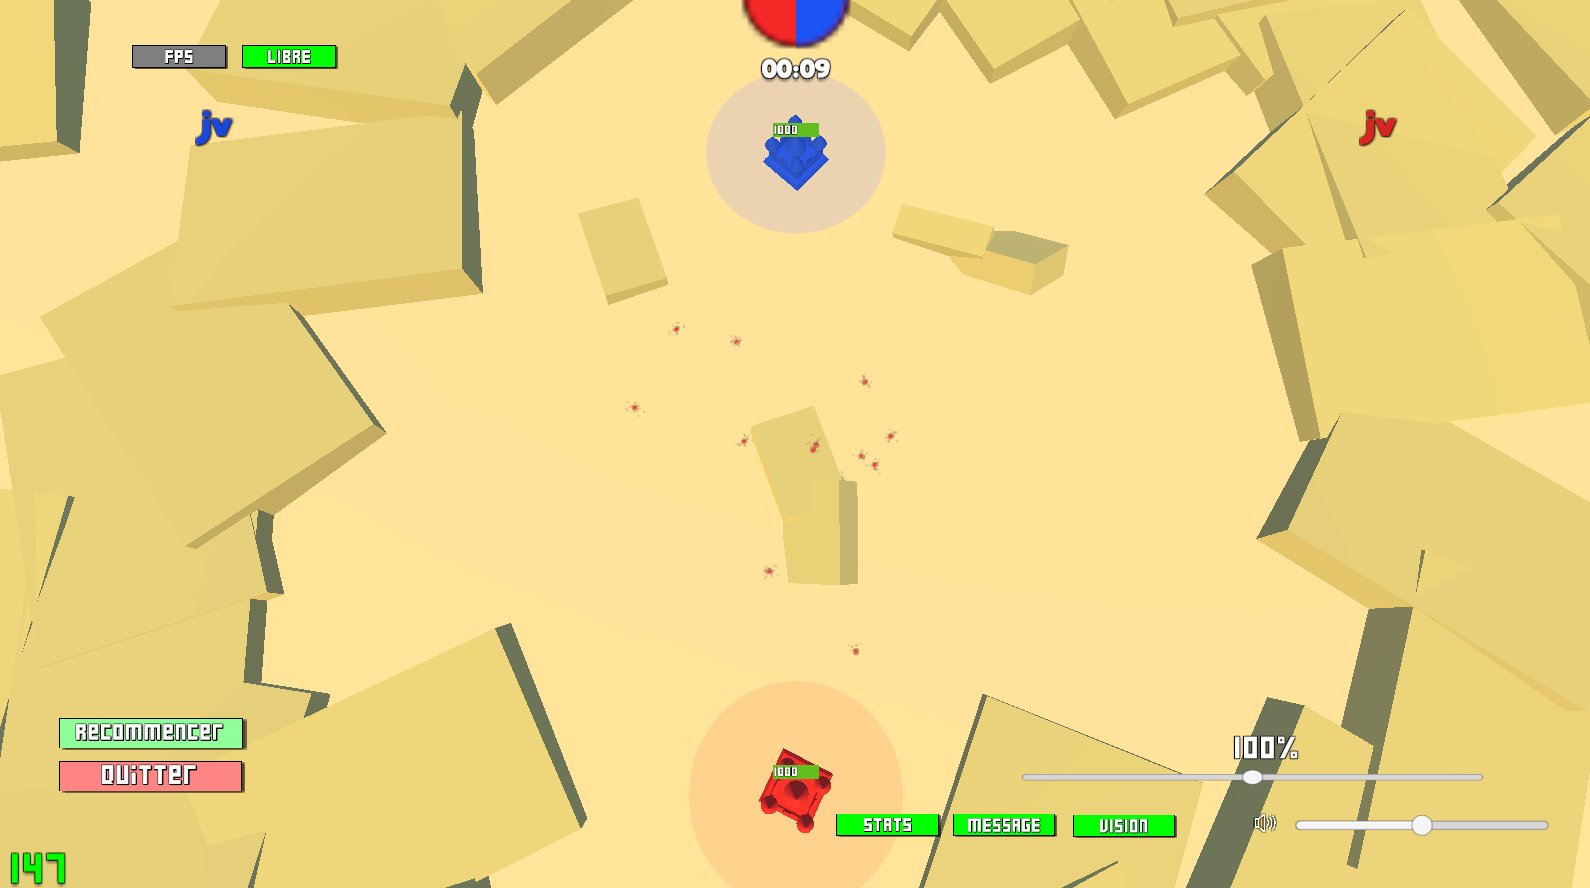
\includegraphics[scale=0.1]{DATA/desolate.png}
  \caption{Desolate}
  \label{fig:sfig2}
\end{subfigure}
\begin{subfigure}{.5\textwidth}
  \centering
  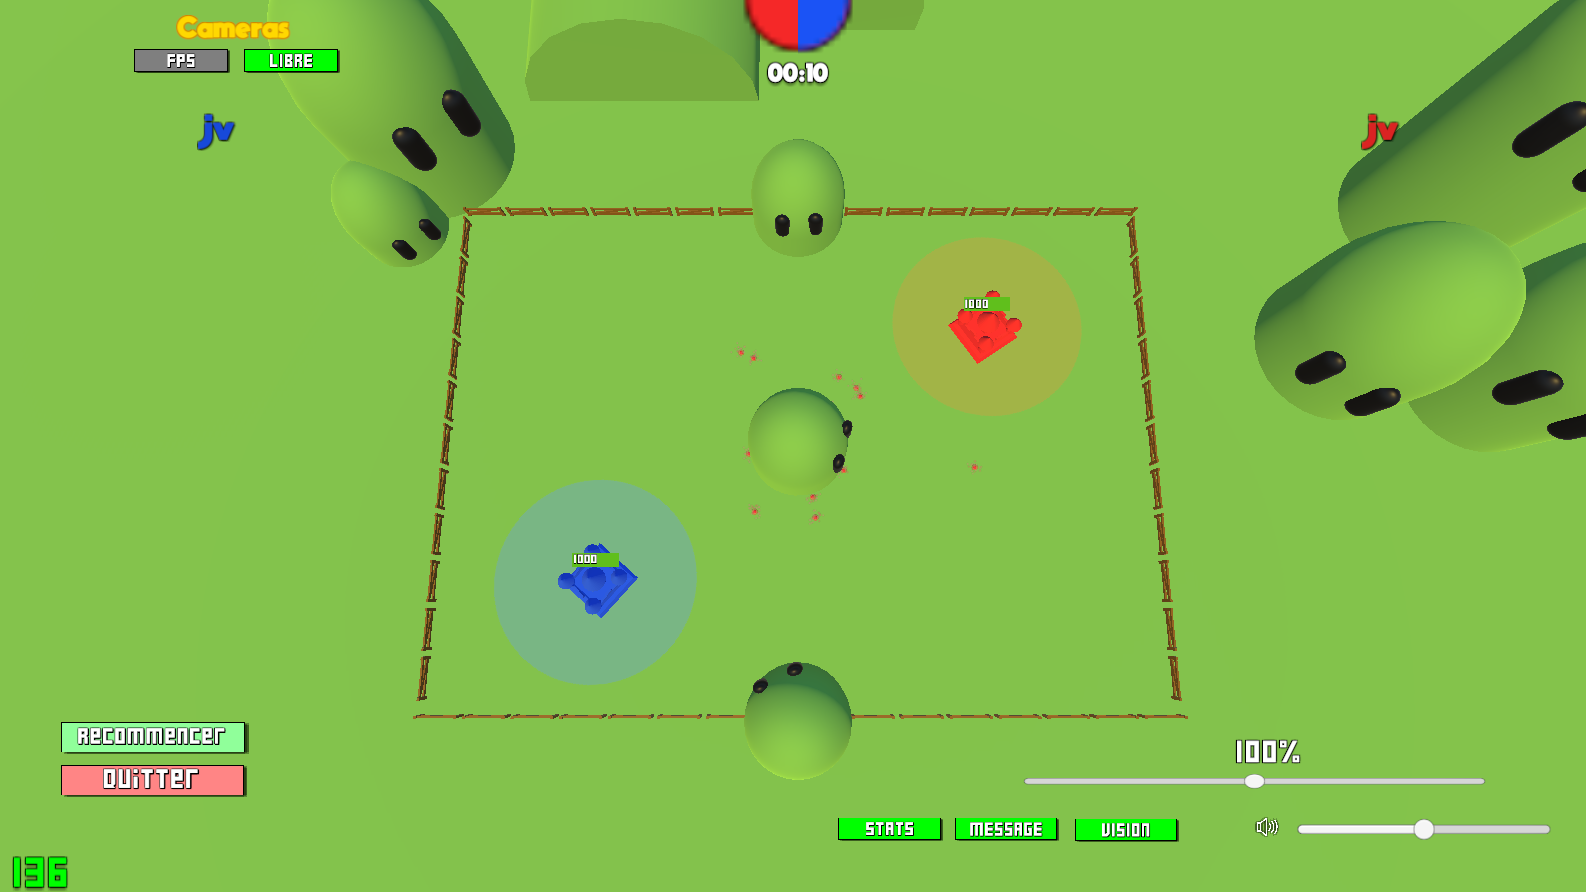
\includegraphics[scale=0.1]{DATA/plaine.png}
  \caption{Plain}
  \label{fig:sfig3}
\end{subfigure}
\newline
\begin{center}
\begin{subfigure}{.5\textwidth}
  \centering
  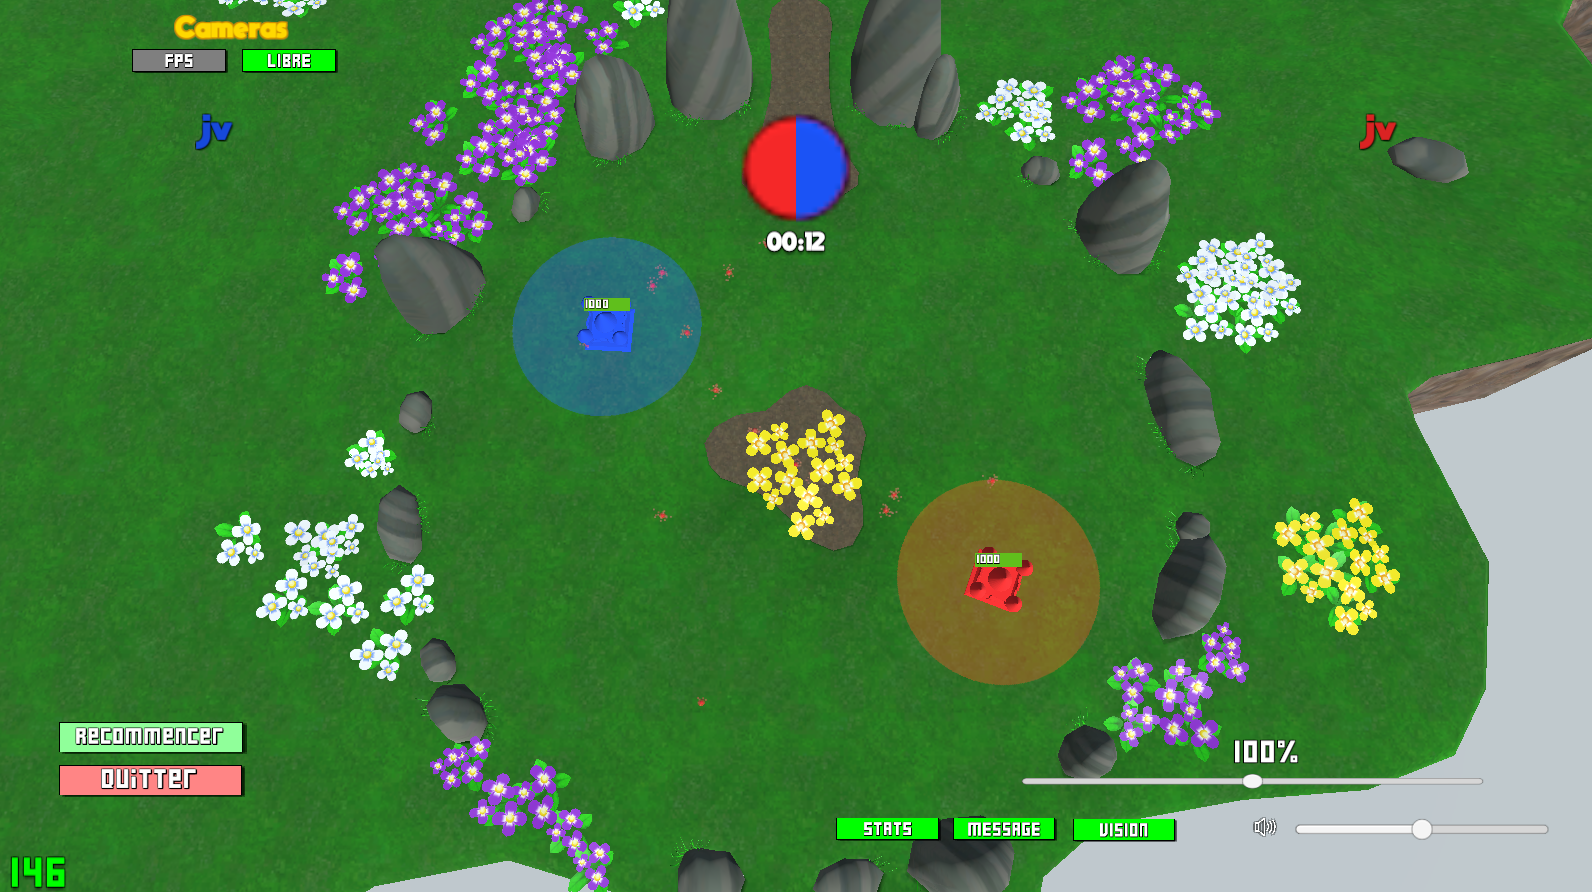
\includegraphics[scale=0.1]{DATA/jardin.png}
  \caption{Garden}
  \label{fig:sfig3}
\end{subfigure}
\begin{subfigure}{.5\textwidth}
  \centering
  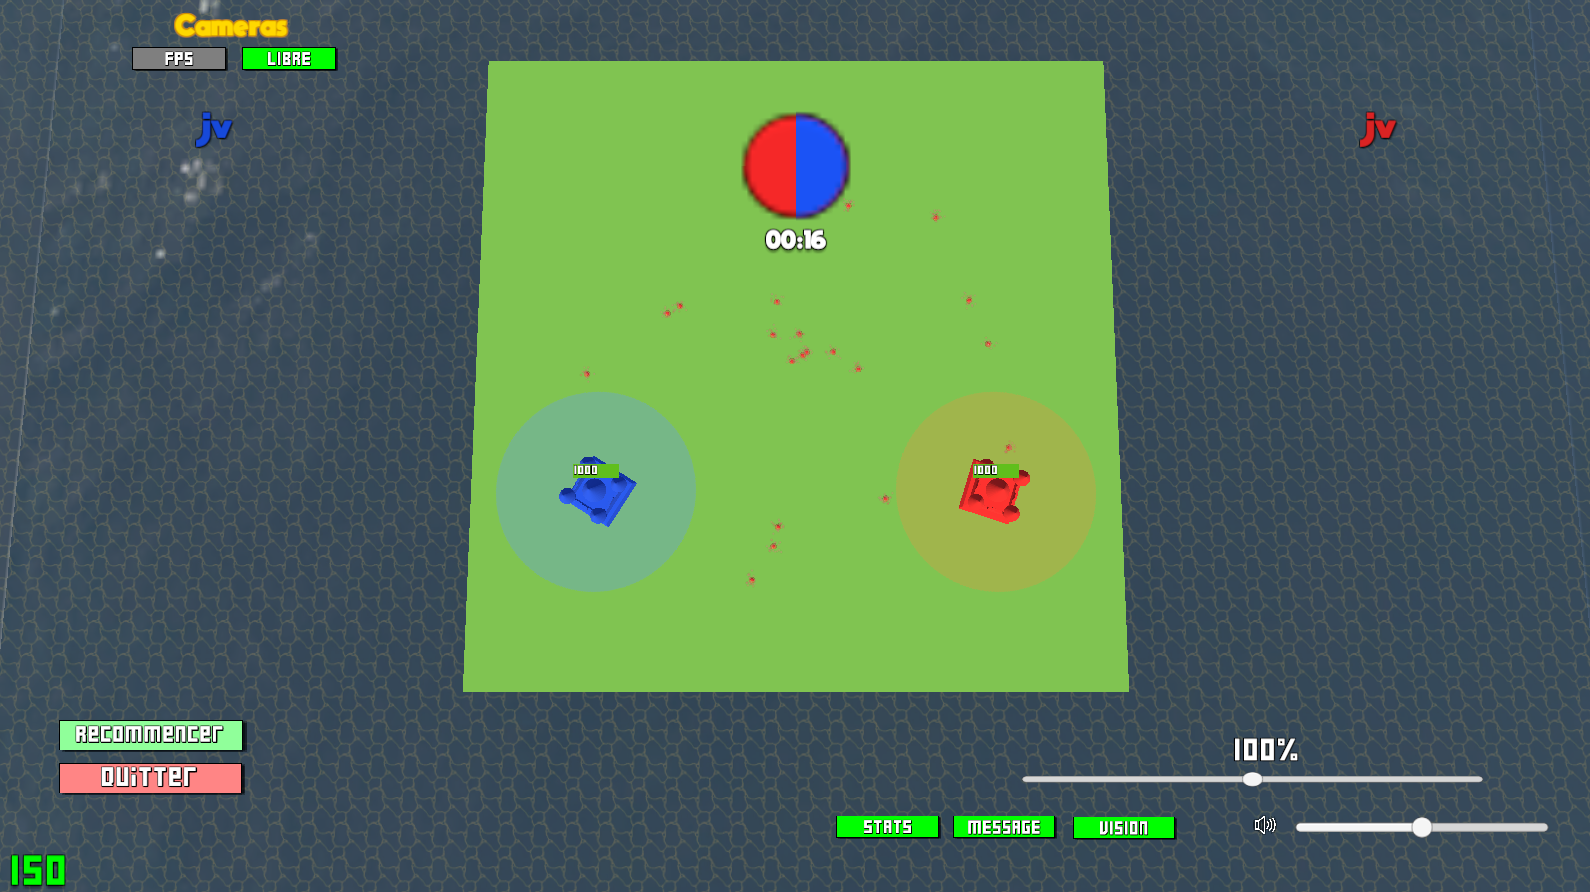
\includegraphics[scale=0.1]{DATA/test.png}
  \caption{Simple}
  \label{fig:sfig3}
\end{subfigure}
\caption{Les cartes jouables de WarBot}
\label{fig:fig}
\end{center}
\end{adjustwidth}
\end{figure}
\paragraph{}

  L’équipe moteur s’est occupée de la création des cartes atuellement présentent dans le projet. La carte Simple était au départ la carte qui servait à faire nos tests dans un environnement où peut d'éléments risquaient de perturber le comportement des agents. Les cartes montagne et Desolate ont été conçues pour permettre plus de possibilités de collision avec le décor. Quand à la carte garden, c'est un model 3D trouvé sur Inernet qui a été ajouté pour vérifier la possibilité d'ajouter des cartes n'étant pas prévues spécifiquement pour notre moteur au départ.

\subsection{Equilibrage}
\paragraph{}
    L’équilibrage est la phase où on ajuste les caractéristiques de chaque unité afin que chacune d’elles possède ses forces et ses faiblesses. Si une unité est trop forte, les joueurs la privilégierons alors que si une unité est trop faible, les joueurs ne voudront pas perdre leur temps à créer un comportement pour une unité qui ne rivalise pas contre ses adversaires. La diversité de comportements possibles serait alors amoindri. \newline
    Dans le cas de WarBot, les statistiques se modifient via un fichier texte sous ce format :
\begin{lstlisting}[frame=single]
Units:
    WarBase:
        MaxHealth: 300
        MaxInventory: 200
        PerceptionRadius: 120
        SpawnDelay: 1.5
    WarTurret:
        MaxHealth: 30
        MaxInventory: 20
        PerceptionRadius: 70
        ReloadTime: 0.1
        Cost: 20
    WarExplorer:
        MaxHealth: 45
        MaxInventory: 100
        PerceptionRadius: 80
        Speed: 65
        Cost: 10
    WarEngineer:
        MaxHealth: 80
        MaxInventory: 100
        PerceptionRadius: 50
        Speed: 30
        SpawnDelay: 4.0
        Cost: 15
    WarHeavy:
        MaxHealth: 100
        MaxInventory: 50
        PerceptionRadius: 85
        Speed: 55
        ReloadTime: 1.0
        Cost: 30
Ressources:
    HealCost: 30
    HealValue: 20
    TakeCount: 20
    GiveCount: 20
    GiveDistance: 30
    MaxRessources: 20
\end{lstlisting}
\paragraph{}
Pour rendre le calcul des statistiques plus simples, nous avons créé un tableur. Pour se faire, nous nous sommes servi de la configuration de la version Java et nous avons calculé un ratio pour chaque statistique de chaque unité en prenant l’explorateur comme référence :

\paragraph{}
\begin{adjustwidth}{-2em}{}
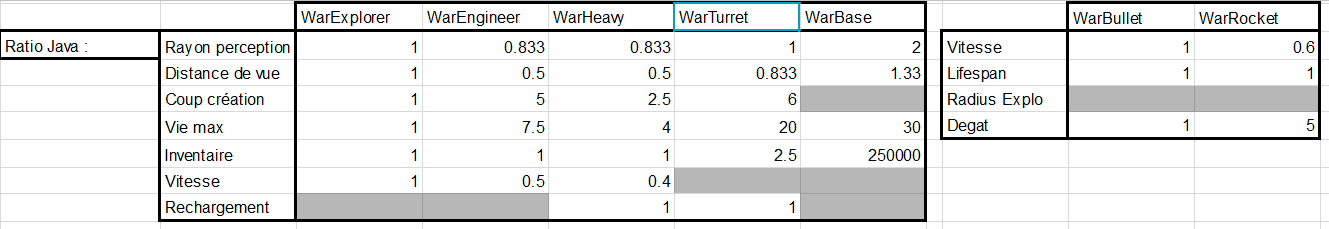
\includegraphics[scale=0.5]{DATA/ratio.png}
\captionof{figure} {Tableau des ratio}
\end{adjustwidth}
\paragraph{}
Nous modifions ensuite les valeurs dans le tableau “valeur par défaut”, ce qui modifie automatiquement les valeurs dans le tableau “calcul via ratio” qui nous sert de référence pour remplir le tableau “Rééquilibrage Unity” dans lequel nous modifions les valeurs à la main pour équilibrer au mieux la version actuelle.

\paragraph{}
\begin{adjustwidth}{-3em}{}
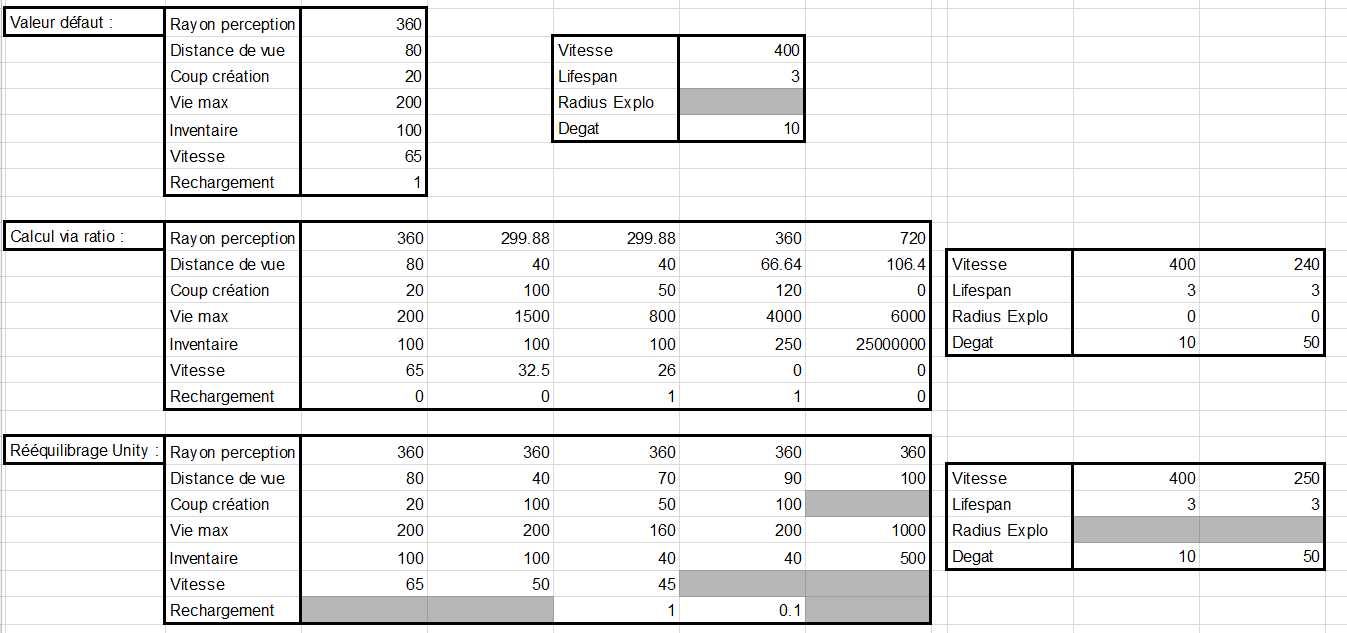
\includegraphics[scale=0.55]{DATA/equilibrage.png}
\captionof{figure} {Calcul des statistiques}
\end{adjustwidth}
\paragraph{}

    La seule unité pour laquelle nous ne calculons pas les statistiques est le WarLight. En effet, cette unité s’est vu rajoutée au cours du projet et n’était donc pas présente lors de la création du tableur. Ses caractéristiques sont donc choisies de manière subjective en se basant sur les statistiques des autres unités. Nous souhaitons que cette unité soit un peu plus lente que les explorateurs. Elle doit également être de résistance moyenne, faire peu de dégâts mais avoir une cadence de tir élevée. \newline
Une fois les unités modifiées, des tests avec des équipes adoptant des stratégies différentes sont effectués. Lors de nos test, nous nous somme rendu compte que l’ajout d’une nouvelle unité rendaient l’équilibrage délicat car cela demande de reconsidérer le rôle de toutes les autres unités. Le fait de ne pas disposer de toutes les possibilités disponibles dans la version Java rend également l’équilibrage difficile car nous ne pouvons pas réellement nous servir d’elle comme référence.
\paragraph{}
Au départ, le WarHeavy semblait presque inutile. En effet, la particularité de cette unité dans la version Java était de pouvoir tirer au-delà de son champs de vision grâce à ses coéquipiers qui pouvaient lui transmettre des coordonnées. L’unité s’orientait alors dans cette direction et faisait feu sur une cible qu’elle ne distinguait pas. Cependant, cette fonctionnalité n’étant pas présente dans notre version, le WarHeavy possédait des caractéristiques trop faibles pour justifier son coût de création. Le plus gros ennui était sa distance de vue trop petite mais en augmentant simplement cette caractéristique, on risquait de créer une unité trop forte qui rendait les WarLight inutiles. \newline
Nous avons donc décidé de réduire l’angle de perception et d’augmenter la portée de son champs de vision. Ainsi, les WarHeavy détectent mieux les ennemis mais sont plus vulnérables aux attaques qui arrivent de côté.
\paragraph{}
Les autres réglages ont plus été des règlements mineurs sur les autres unités pour obtenir des parties plus dynamique. On a par exemple légèrement augmenté les dégâts des unités offensives pour que les parties se terminent plus rapidement.
\paragraph{}
En plus de l’équilibrage des unités, on a cherché à modifier de manière générale les propriétés des unités pour obtenir des expériences de jeux différentes. Tout d’abord, on a noté les performances de l’équilibrage de base afin de pouvoir les comparer. Nous avons effectué cette acquisition de données sur la carte “Mountain” qui est une carte de taille moyenne et ne comportent pas d’obstacle. Le comportement de l’équipe de test restait basique : les explorateurs s’aident pour la récolte en partageant leur position quand ils ramassent une ressource, les unités offensives partagent la position des ennemis qu’ils attaquent et la tour se soigne et créé un explorateur quand elle le peut. Avec tous ces facteurs, une partie dure environ 1min30.
\paragraph{}
Nous avons ensuite voulu essayer un mode où des erreurs de comportements seraient beaucoup plus punitives. On s’est orienté vers une réduction des points de vie. Avec ce réglage, le nombre de coups en fonction de son type et de l’unité attaqué devenait le suivant : 


\paragraph{}
\begin{adjustwidth}{-3em}{}
\begin{center}
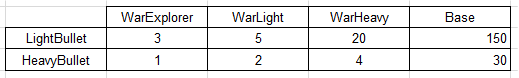
\includegraphics[scale=1]{DATA/coutUnit.png}
\captionof{figure} {Nombre de coups pour tuer une unité en fonction de son type}
\end{center}
\end{adjustwidth}
\paragraph{}

\paragraph{}
Comme excepté, la durée des parties était plus courte et passait généralement en dessous de la barre de la minute. Cependant, avec des points de vie aussi faibles, on s’est demandé si certains comportements atypiques pouvaient apparaître, voire avoir un comportement qui est clairement supérieur aux autres.  On s’est alors rappelé du concours WarBot que l’on a fait au semestre précédent sous Java. Une des équipes avait une stratégie où leur base sacrifiait quasiment l’ensemble de ces points de vie pour créer un maximum d’unité et finir la partie avant que l’équipe adverse est le temps de riposter. On a donc recréé cette équipe avec notre version de Warbot et on s’est rendu compte qu’elle était très efficace avec un taux de victoire supérieur à 80\% sur 20 parties. Deux questions se sont donc posé : est-ce notre équipe de base qui est trop faible ou est-ce ce comportement qui est particulièrement trop fort ?
\paragraph{}
On a donc créé d’autres équipes pour répondre à ces questions : une équipe du même type mais sans la communication, une équipe plus avancée avec une base qui gère mieux ces points de vie et la création d’unités et une équipe assez faible où il n’y a aucune communication et aucune création d’unité au niveau de la base. Avec ces équipes, on visait le classement suivant :
\begin{itemize}
\item Première place : l’équipe avancée et l’équipe “sacrifice” avec communication,
\item Deuxième place : l’équipe “sacrifice” avec communication,
\item Troisième place  : l’équipe de base 
\item Quatrième place : l’équipe “sacrifice” sans communication,
\item Cinquième place : l’équipe faible
\end{itemize}
\paragraph{}
  Ce classement se base sur un principe de base que l’on souhaite sur WarBot : la communication est un élément central du jeu et on souhaite récompenser les joueurs qui l’utilisent. C’est pour cela que les trois équipes utilisant ce principe sont dans le haut du classement. Ensuite, les équipes “sacrifice” doivent tout de même rester moins fiables que des équipes plus complexes tout en l’heure laissant l’occasion de gagner sur un “coup de poker”.  On a tout d’abord fait affronter les équipes communication/sans communication de chaque type. Au niveau des équipes basique/avancé, on obtient le résultat escompté : une domination de la part de l’équipe avancé. Pour les équipes “sacrifices”, le résultat était plus aléatoire. En effet, avec aussi peu de points de vie, un comportement aléatoire sans communication, même si peu d’unité, trouve plus rapidement la base adverse et ne laisse pas le temps à l’équipe adverse la possibilité de répliquer. De son côté, l’équipe faible gagnait seulement contre l’équipe sacrifice sans communication dans de rares cas. On retrouvait donc le classement pré-établi plus tôt. 
  \paragraph{}
  Au final, on en a conclu que c’était notre équipe de base qui était trop faible et qu’une bonne gestion de la communication et de ses ressources étaient souvent plus pertinentes. On a refait les mêmes tests avec l'équilibrage basique (plus de points de vie). Comme avec l’équilibrage précédent, le classement entre les équipes fut le même. De plus, l’équipe “sacrifice” avec communication semblait prendre plus facilement l'avantage sur l’équipe “sacrifice” sans communication. On a donc repris cet équilibrage comme base. Le public visé étant aussi des jeunes, on ne souhaite pas que l’expérience de jeu soit trop frustrante et trop punitive. Il est cependant toujours possible de basculer vers l’autre équilibrage facilement pour créer d’autres types de tournoi et/ou vérifier la fiabilité d’une équipe face à d’autres rythmes de jeu. 
  

\paragraph{}
\begin{adjustwidth}{-3em}{}
\begin{center}
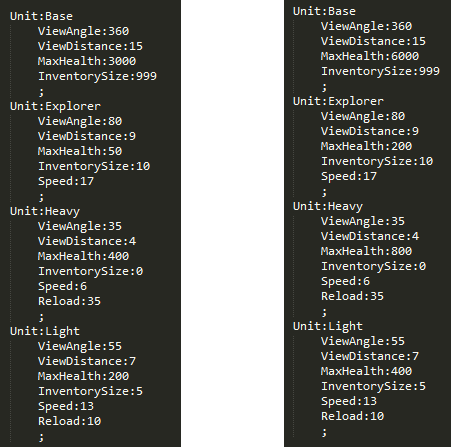
\includegraphics[scale=1]{DATA/EquilibrageComp.png}
\captionof{figure} {A gauche, équilibrage punitif. A droite, équilibrage choisi}
\end{center}
\end{adjustwidth}
\paragraph{}


\newpage

\part{L'avenir du projet}
\chapter{Amélioration possible}
\section{Interpreter}
Bien sûr de nombreuses choses restent à mettre en place et à améliorer dans ce projet. Maintenant que les développeurs ont une base permettant d’ajouter facilement des modes de jeux, des cartes et des unités, les possibilités d’améliorations de MetaBot très grandes. 
\paragraph{}
Au sein du travail de l’équipe interpréteur, de grosses modifications sur la condition de victoire “Course aux ressources” sont possibles, afin de le transformer comme un vrai mode de jeu, et pas simplement un changement rattaché au mode de jeu Warbot. 
\paragraph{}
L’ajout de nouvelles caméras est bien sûr faisable si l’imagination des groupes suivant trouve une caméra intéressante. 
\paragraph{}
L’interpréteur devra lui être mis à jour avec l’ajout de possibilités dans le langage, mais il suffira pour l’ajout de primitives telles qu’elles sont dans le projet actuel.
\paragraph{}
Il sera aussi nécessaire comme indiqué plus haut, de remettre en place une fenêtre pour afficher les matchups entre équipes, de manière à ne pas surcharger l’affichage. Il serait aussi bien d’étendre le fonctionnement des ELO point pour le faire fonctionner à 3 ou 4 joueurs, ce qui est pas forcément dans l’idée initiale du système ELO, mais qui sera plus cohérent par rapport au projet
\paragraph{}
Enfin, le maintien à jour des traductions sera nécessaire au fur et à mesure du développement, et bien sûr l’ajout de nouvelles langues facilement dès que cela est nécessaire.
\paragraph{}
Pour la gestion de la fin du jeu, un travail restera nécessaire pour rendre l’initialisation des éléments d’interfaces plus propre. De plus,actuellement la fin du jeu fonctionne sur la condition de victoire car nous n’avons pas deux modes différents, mais il faudra juste changer l’appel au test et à l'exécution de la fin de jeu dans l’ “Update” du script.

\section{Game Design}

\paragraph{}
  Evidemment, la partie test de MetaBot va subir d’importante amélioration dans l’avenir car les prochains étudiants qui travailleront sur ce projet trouveront de nouveaux bugs.
\paragraph{}
Il reste à implémenter les unités manquantes de la version actuelles comme les Tourelles ou les Kamikazes qui demanderont alors de revoir l’équilibrage pour que chaque unité possède une force et un intérêt stratégique similaire à ceux des autres unités.
\paragraph{}
 Le système de groupe et d’objectif ainsi que l’ajout des primitives évoqués dans la partie “Améliorations demandées” permettraient d’augmenter le nombre de possibilité des joueurs ce qui permettra de commencer à voir des équipes radicalement différentes.
\paragraph{}
Bien sûr, il est toujours possible de concevoir de nouveaux modes de jeu et de nouvelles cartes. Il pourrait être intéressant que le mode de course aux ressources soit poussé plus loin pour former un mode à part car les unités offensives sont beaucoup moins intéressantes dans ce mode de jeu.
\paragraph{}
Le mode de jeu de coopération nous semble encore trop peu intéressant notamment à cause des transporteurs qui devraient avoir un rôle plus important. Malheureusement, en laissant le contrôle à l'unité qu'elle transporte, cette unité est plus un outil de l'équipe A qu'une unité de l'équipe B.


\chapter{Conclusion}
\section{Bugs}
Bien sûr de nombreux bugs vont subsister lors de la modification et l’ajout de fonctionnalités que nous ne voyons pas encore, mais nous pourrons répondre aux questions des prochaines équipes travaillant sur le projet si besoin.

\section{Point final}
Ce projet a été une grande expérience pour nous tous.\newline
Ce fut une joie pour certains d’entre nous,qui n’avaient pas encore travaillé avec des outils comme Unity,  de pouvoir se lancer dans la découverte du développement d’un jeu comme Warbot.\newline
L’apprentissage de nouveaux outils et de nouvelles méthodes de programmation qui peuvent dépayser un développeur a été une expérience formidable pour chacun.
\paragraph{}
Travailler à 8 fut une expérience enrichissante pour tous les membres de l’équipe qui ont rarement voire jamais eu l’occasion de travailler à plus de 4 sur un même projet. \newline
Être autant sur ce projet nous a permis de nous confronter aux problèmes de communications mais aussi de diversifier énormément le type de travail demandé à chacune des sous-équipes de 2 formées pendant ce projet. De plus les réunions hebdomadaires ont été l’occasion de comprendre les enjeux et les méthodes de travail de chaques parties nécessaires au développement de WarBot. 
\paragraph{}
L’ensemble du projet à été réalisé sous une méthode de développement Agile, qui a été une expérience nouvelle pour certains d’entre nous.\newline
Le respect des délais pour l’implémentation de fonctionnalités, l’assurance d’avoir un jeu qui pourra être lancé à chaque réunion avec notre encadrant sont des contraintes auxquelles il a fallu s’habituer. \newline
Le jeu a ainsi été utilisable à chaque réunion, quelques soit les fonctionnalités implémentées durant la semaine qui précédait. 
\paragraph{}
Toute l’équipe souhaite donc remercier M. Ferber pour nous avoir permis de participer à son projet de portage de WarBot sous le moteur de jeu Unity, en plus de son expérience et de ses nombreux conseils. \newline
Nous souhaitons aussi remercier l’équipe qui a travaillé sur le moteur et l’interface du jeu, pour l’aide qu’ils ont pu nous apporter, ainsi que l’équipe de l’année précédente qui nous ont permis de nous aiguiller sur comment améliorer leur version du projet. \newline
Enfin, nous remercions M. Lafourcade pour l’expérience qu’il a apporté à tout le monde par l’organisation de l’UE TER.

\newpage
\part{Annexe}
\section{Captures d'écrans du jeu}
Voici un ensemble de capture d’écrans, afin que vous puissiez voir le jeu tel qu’il est a la fin de la rédaction de ce rapport.

\paragraph{}
\begin{adjustwidth}{-3em}{-3em}
\begin{center}
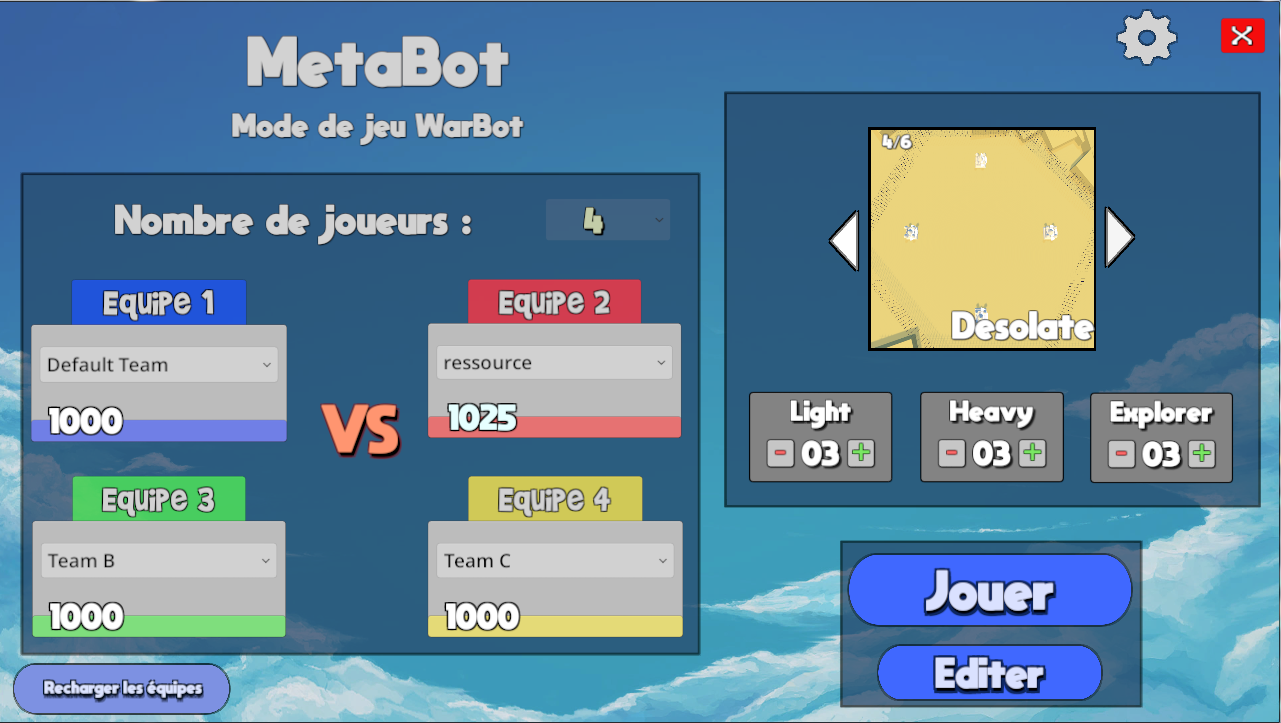
\includegraphics[scale=0.5]{DATA/menuprincipal.png}
\captionof{figure} {Menu Principal du jeu}
\end{center}
\end{adjustwidth}
\paragraph{}


\paragraph{}
\begin{adjustwidth}{-3em}{-3em}
\begin{center}
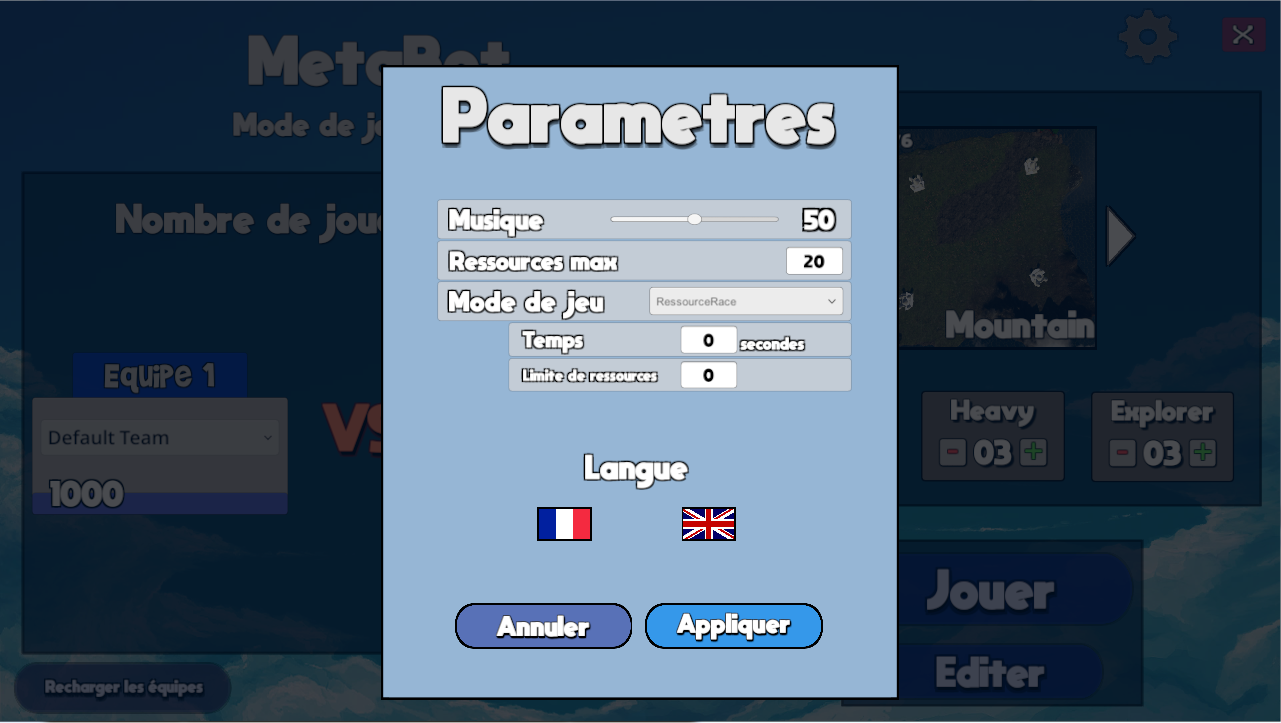
\includegraphics[scale=0.5]{DATA/menuparametre.png}
\captionof{figure} {Menu Paramètres du jeu}
\end{center}
\end{adjustwidth}
\paragraph{}

\paragraph{}
\begin{adjustwidth}{-3em}{-3em}
\begin{center}
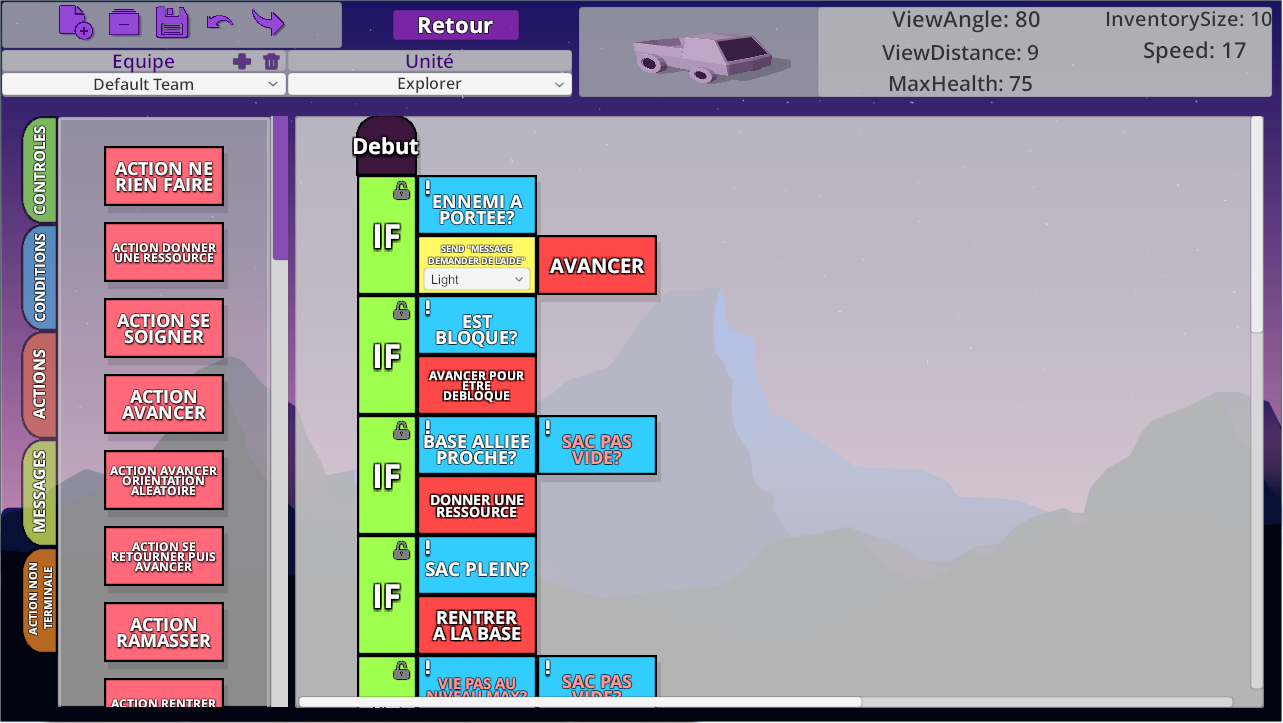
\includegraphics[scale=0.5]{DATA/editeurcomportement.png}
\captionof{figure} {Editeur de comportement du jeu}
\end{center}
\end{adjustwidth}
\paragraph{}


\paragraph{}
\begin{adjustwidth}{-3em}{-3em}
\begin{center}
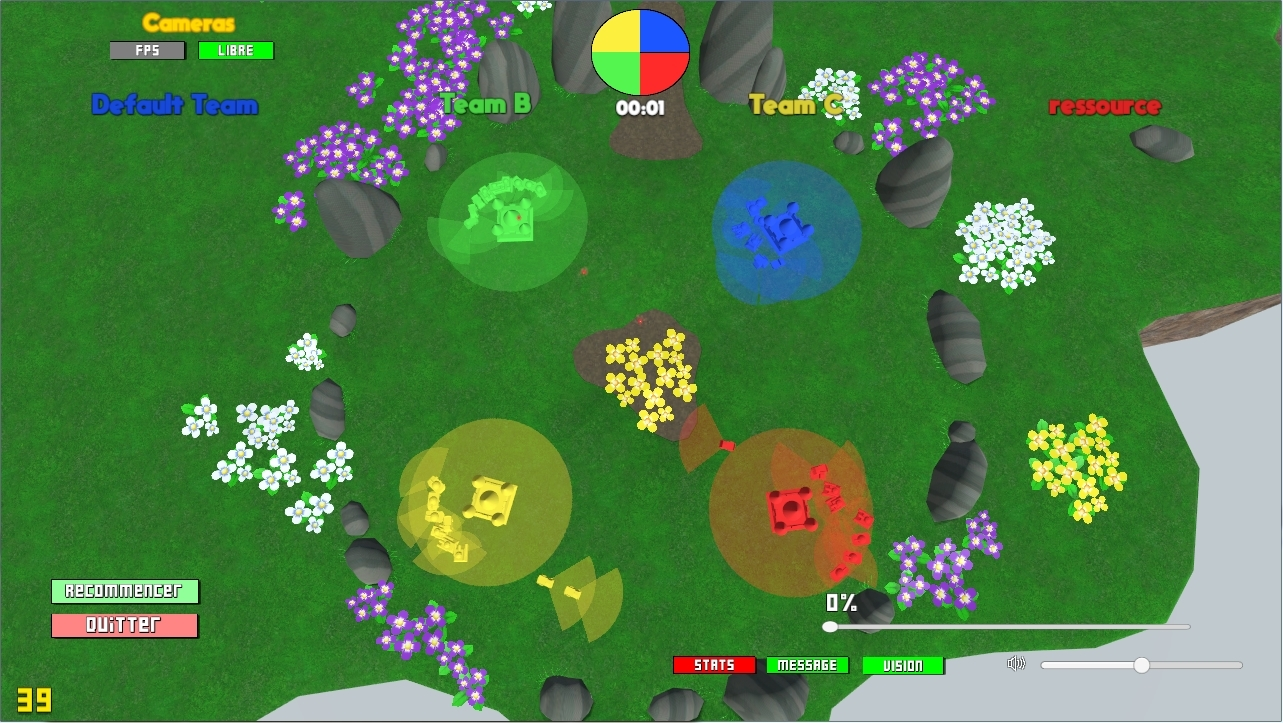
\includegraphics[scale=0.3]{DATA/enjeu.png}
\captionof{figure} {Interface en jeu sur la carte “Garden”}
\end{center}
\end{adjustwidth}
\paragraph{}

\paragraph{}
\begin{adjustwidth}{-3em}{-3em}
\begin{center}
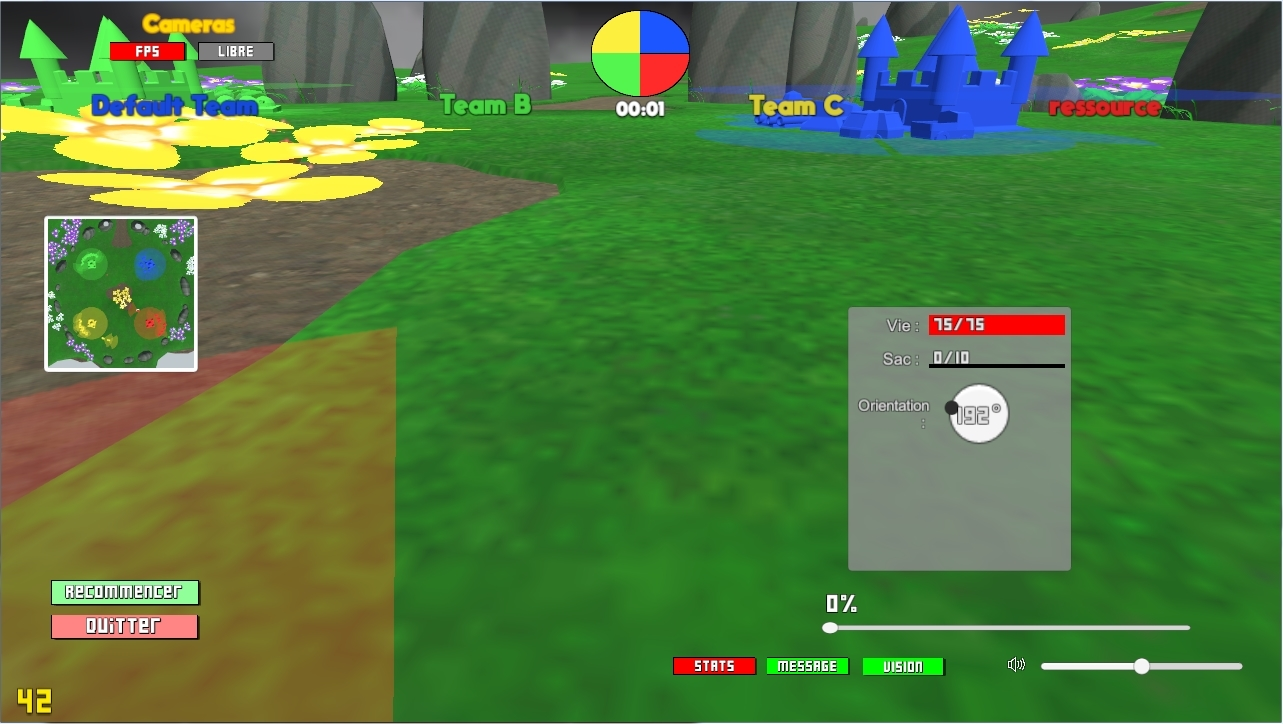
\includegraphics[scale=0.3]{DATA/enjeufps.png}
\captionof{figure} {Interface en vue première personne sur la carte “Garden”}
\end{center}
\end{adjustwidth}
\paragraph{}


\section{Point importants du code}


\begin{lstlisting}[frame=single]
 public override Instruction whichInstruction(string unitName, XmlNode ins)
    {
        List<string> l_conditions = new List<string>();
        List<MessageStruct> l_MsgStruct = new List<MessageStruct>();
        List<string> l_actions = new List<string>();

        foreach (XmlNode x in ins.ChildNodes)
        {

            if (x.Name.Contains("parameters"))#Partie condition de l'instruction
            {
                foreach (XmlNode c in x)
                    l_conditions.Add(c.Name);
            }

            if (x.Name.Contains("message"))#Partie action non temrinale de l'instruction
            {
                foreach (XmlNode c in x)
                {
                    l_MsgStruct.Add(new MessageStruct(c.Name, c.FirstChild.Name));
                }
            }

            if (x.Name.Contains("actions"))#Partie action terminale de l'instruction
            {
                foreach (XmlNode c in x)
                    l_actions.Add(c.Name);
            }
        }
        if (l_actions.Count == 0)
        {
            return new Instruction(l_conditions.ToArray(), l_MsgStruct.ToArray());
        }
        return new Instruction(l_conditions.ToArray(), l_MsgStruct.ToArray(), l_actions[0]);

    }
\end{lstlisting}
\captionof{figure} {Fonction qui extrait les instructions des noeud des unités}

\begin{lstlisting}[frame=single]
   #Creer un comportement a partir d'un fichier xml
    public override Dictionary<string, List<Instruction>> xmlToBehavior(string teamName, string path)
    {
        string l_fileName = whichFileName(teamName, path);

        if (l_fileName.Equals(""))
            l_fileName = teamName.Replace(".wbt", "") + Constants.xmlExtension;

        Dictionary<string, List<Instruction>> behavior = new Dictionary<string, List<Instruction>>();

        string pathtmp = path;
        l_fileName = path +"/" +  l_fileName.Replace(path, "");
        using (var stream = new FileStream(l_fileName, FileMode.Open))
        {
            Load(stream);
            XmlNodeList l_units = GetElementsByTagName(Constants.nodeUnit);
            stream.Close();

            for (int i = 0; i < l_units.Count; i++)
            {
                string l_unitName = l_units.Item(i).Attributes.Item(0).Value;
                behavior.Add(l_unitName, xmlToUnitBehavior(teamName, path, l_unitName));
            }
        }

        return behavior;
    }

\end{lstlisting}
\captionof{figure} {Transformation d’un fichier XML en comportement}

\begin{lstlisting}[frame=single]
  #Recupere le comportement d'une unite dans un fichier xml d'une equipe
    public List<Instruction> xmlToUnitBehavior(string teamName, string path, string unitName)
    {
        string l_fileName = whichFileName(teamName, path);

        if (l_fileName.Equals(""))
            l_fileName = teamName;

        List<Instruction> l_behavior = new List<Instruction>();
        l_fileName = teamName.Replace(".wbt", "") + Constants.xmlExtension;
        l_fileName = path + "/" + l_fileName.Replace(path, "");

        using (FileStream stream = new FileStream(l_fileName, FileMode.Open))
        {
            Load(stream);
            XmlNode l_unitBehavior = SelectSingleNode("//" + Constants.nodeUnit + "[@" + Constants.attributeName + "='" + unitName + "']");
            if (l_unitBehavior != null && l_unitBehavior.HasChildNodes)
            {
                foreach (XmlNode ins in l_unitBehavior.ChildNodes)
                {
                    l_behavior.Add(whichInstruction(unitName, ins));
                }

            }

            stream.Close();
        }
        return l_behavior;
    }
\end{lstlisting}
\captionof{figure} {Fonction support de la transformation de XML en comportement}

\begin{lstlisting}[frame=single]
  public override void behaviorToXml(string teamName, string path, string unitName, List<Instruction> behavior)
    {
        string l_fileName = whichFileName(teamName, path);

        if (l_fileName.Equals(""))
        {
            l_fileName = teamName + Constants.xmlExtension;
            generateEmptyFile(teamName, path);
        }

        l_fileName = whichFileName(teamName, path);
        Load(l_fileName);

        XmlNode l_node = SelectSingleNode("//" + Constants.nodeUnit + "[@" + Constants.attributeName + "='" + unitName + "']");
        if (l_node == null)
            l_node = CreateElement(Constants.nodeUnit);

        l_node.RemoveAll();

        XmlAttribute l_name = CreateAttribute(Constants.attributeName);
        l_name.Value = unitName;
        l_node.Attributes.Append(l_name);

        foreach (Instruction i in behavior)
            l_node.AppendChild(ImportNode(i.xmlStructure(), true));

        XmlNode l_embbed = FirstChild;
        l_embbed.AppendChild(l_node);

        Save(l_fileName);
    }
\end{lstlisting}
\captionof{figure} {Transformation d’un comportement en fichier XML}



\begin{lstlisting}[frame=single]
 public bool removeFPS()
    {
        if (fps)
        {
            transform.SetPositionAndRotation(backPosition, backRotation);
            fps = false;
            removeStuck();
            Cursor.lockState = back;
            minimap.gameObject.SetActive(false);
            unit = null;
            mainCam.GetComponent<FollowCamera>().enabled = true;
            select.GetComponent<SpriteRenderer>().color = new Color(select.GetComponent<SpriteRenderer>().color.r, select.GetComponent<SpriteRenderer>().color.g, select.GetComponent<SpriteRenderer>().color.b, 0);
            return true;
        }

        return false;
    }

    #Quitter le mode Camera Libre
    public bool removeStuck()
    {
        if (stuck)
        {
            if (fps)
            {
                removeFPS();
            }
            transform.SetPositionAndRotation(backPosition, backRotation);
            stuck = false;
            mainCam.GetComponent<FollowCamera>().enabled = true;

            return true;
        }

        return false;
    }

   #Rentrer en mode Camera Libre
    public bool goStuck()
    {
        if (!stuck && !fps)
        {
            if (mainCam.GetComponent<FollowCamera>().enabled)
                mainCam.GetComponent<FollowCamera>().enabled = false;
            stuck = true;
            fps = false;
            Camera.main.transform.rotation = Quaternion.Euler(80, 0, 0);
            return true;
        }

        return false;
    }

\end{lstlisting}
\captionof{figure} {Fonctions de transition d’une caméra à l’autre}

\begin{lstlisting}[frame=single]
 #traitement de la camera fps
        if (fps)
        {
            Camera.main.transform.position = new Vector3(unit.gameObject.transform.position.x, unit.gameObject.transform.position.y + 3, unit.gameObject.transform.position.z+1);
            select.transform.position = new Vector3(unit.transform.position.x, unit.transform.position.y, unit.transform.position.z);

            yaw += speedH * Input.GetAxis("Mouse X");
            pitch -= speedV * Input.GetAxis("Mouse Y");
            transform.eulerAngles = new Vector3(+25.0f, yaw, 0.0f);
        }

       #traitement de la camera libre
        if (stuck)
        {
            if (Input.GetAxis("Mouse ScrollWheel") < 0f) #arriere
            {
                GameObject ground = GameObject.FindGameObjectWithTag("Ground");
                Vector3 dist = Camera.main.transform.position - ground.transform.position;
                if (!(dist.magnitude > backPosition.y + backPosition.y/2))
                {
                    Camera.main.transform.position = new Vector3(Camera.main.transform.position.x, Camera.main.transform.position.y - 10 * Input.GetAxis("Mouse ScrollWheel"), Camera.main.transform.position.z);
                }
            }
            else if (Input.GetAxis("Mouse ScrollWheel") > 0f) // avant
            {
                        float dist = Camera.main.transform.position.y - terrain.bounds.size.y;
                        if (!(dist < 1))
                        {
                            Camera.main.transform.position = new Vector3(Camera.main.transform.position.x, Camera.main.transform.position.y - 10 * Input.GetAxis("Mouse ScrollWheel"), Camera.main.transform.position.z);
                        }
            }
            

            if (Input.mousePosition.x <= 2 && Camera.main.transform.position.x > backPosition.x - terrain.bounds.size.x / 4)
                Camera.main.transform.position = new Vector3(Camera.main.transform.position.x - speed, Camera.main.transform.position.y, Camera.main.transform.position.z);
            if (Input.mousePosition.y <= 2 && Camera.main.transform.position.z > backPosition.z - terrain.bounds.size.z / 4)
                Camera.main.transform.position = new Vector3(Camera.main.transform.position.x , Camera.main.transform.position.y , Camera.main.transform.position.z - speed);

            if (Input.mousePosition.x >= Screen.width - 2 && Camera.main.transform.position.x < backPosition.x + terrain.bounds.size.x / 4)
                Camera.main.transform.position = new Vector3(Camera.main.transform.position.x + speed, Camera.main.transform.position.y, Camera.main.transform.position.z);
            if (Input.mousePosition.y >= Screen.height - 2 && Camera.main.transform.position.z < backPosition.z + terrain.bounds.size.z / 4)
                Camera.main.transform.position = new Vector3(Camera.main.transform.position.x, Camera.main.transform.position.y , Camera.main.transform.position.z + speed);
        }
    }

\end{lstlisting}
\captionof{figure} {Traitement des 2 caméras}

\begin{lstlisting}[frame=single]
    public void Traduction()
    {
        foreach (Langage l in GameObject.Find("GameManager").GetComponent<LangageLoader>().langues)
        {
            if (l.langue.Equals(langue))
            {
                foreach (Traduction t in l.trads)
                {
                    if (textOriginal.Equals(t.cle))
                    {
                        traduction = t.valeur;
                        return;
                    }
                }
            }
        }

        traduction = textOriginal;
    }

\end{lstlisting}
\captionof{figure} {Fonction de traduction}

\begin{lstlisting}[frame=single]
  public Langage readFile(string Language)
    {
        Langage l_lang = new Langage();
        l_lang.langue = Language;
        l_lang.trads = new List<Traduction>();

        if (!checkFile(Language))
            return new Langage();
            
        string[] lines = System.IO.File.ReadAllLines(Application.streamingAssetsPath + Constants.langDirectory + Language + ".txt");

        foreach (string line in lines)
        {
            if (!(line.Contains("#")))
            {
                string [] tmp = line.Split('=');
                Traduction l_tmp = new Traduction();
                l_tmp.cle = tmp[0].Replace("\t","") ;
                l_tmp.valeur = tmp[1];
                l_lang.trads.Add(l_tmp);
            }
        }

        return l_lang;
    }

\end{lstlisting}
\captionof{figure} {Lecture des traductions dans les fichiers}

\begin{lstlisting}[frame=single]
[System.Serializable]
public struct Langage
{
    public string langue;
    public List<Traduction> trads;
}

[System.Serializable]
public struct Traduction
{
    public string cle;
    public string valeur;


\end{lstlisting}
\captionof{figure} {Structure des traductions}

\begin{lstlisting}[frame=single]
    public void WriteStats(string[] Teams, string Winner, int NbTeam)
    {
        foreach (string Team in Teams)
        {
                if (!System.IO.File.Exists(Application.streamingAssetsPath + "/Stats/" + Team + ".stat"))
                    System.IO.File.Create(Application.streamingAssetsPath + "/Stats/" + Team + ".stat");
            int i = 0;
            string[] Stats = System.IO.File.ReadAllLines(Application.streamingAssetsPath + "/Stats/" + Team + ".stat");
            bool isInT0 = false;
            bool isInT1 = false;
            bool isInT2 = false;
            bool isInT3 = false;
            foreach (string Stat in Stats)
            {
                string[] DetailStat = Stat.Split('/');
                if (DetailStat[0] == Teams[0])
                {
                    isInT0 = true;
                    int numVal = int.Parse(DetailStat[1]);
                    numVal++;
                    DetailStat[1] = numVal.ToString(); //NbMatch
                    if (Team == Winner)
                    {
                        numVal = int.Parse(DetailStat[2]);
                        numVal++;
                        DetailStat[2] = numVal.ToString(); #NbVictoire
                    }
                }
                if (DetailStat[0] == Teams[1])
                {
                    isInT1 = true;
                    int numVal = int.Parse(DetailStat[1]);
                    numVal++;
                    DetailStat[1] = numVal.ToString(); //NbMatch
                    if (Team == Winner)
                    {
                        numVal = int.Parse(DetailStat[2]);
                        numVal++;
                        DetailStat[2] = numVal.ToString(); #NbVictoire
                    }
                }
                if (NbTeam >= 3 && DetailStat[0] == Teams[2])
                {
                    isInT2 = true;
                    int numVal = int.Parse(DetailStat[1]);
                    numVal++;
                    DetailStat[1] = numVal.ToString(); #NbMatch
                    if (Team == Winner)
                    {
                        numVal = int.Parse(DetailStat[2]);
                        numVal++;
                        DetailStat[2] = numVal.ToString(); #NbVictoire
                    }
                }
                if (NbTeam >= 4 && DetailStat[0] == Teams[3])
                {
                    isInT3 = true;
                    int numVal = int.Parse(DetailStat[1]);
                    numVal++;
                    DetailStat[1] = numVal.ToString(); #NbMatch
                    if (Team == Winner)
                    {
                        numVal = int.Parse(DetailStat[2]);
                        numVal++;
                        DetailStat[2] = numVal.ToString(); #NbVictoire
                    }
                }
    
                
                Stats[i] = DetailStat[0] + '/' + DetailStat[1] + '/' + DetailStat[2];
                i++;
            }
            if (i > 0) i--;
            if (!isInT0 && Team != Teams[0])
            {
                i++;
                System.Array.Resize(ref Stats, i);
                //Stats = (string[]) ResizeArray(Stats, new string[] { i });
                if (Team == Winner) Stats[i-1] = Teams[0] + "/1/1";
                else Stats[i-1] = Teams[0] + "/1/0";//--------------------------------------------------------------------------------------
            }
            if (!isInT1 && Team != Teams[1])
            {
                i++;
                System.Array.Resize(ref Stats, i);
                //Stats = (string[]) ResizeArray(Stats, new string[] { i });
                if (Team == Winner) Stats[i-1] = Teams[1] + "/1/1";
                else Stats[i-1] = Teams[1] + "/1/0";
            }
            if (NbTeam >= 3 && !isInT2 && Team != Teams[2])
            {
                i++;
                System.Array.Resize(ref Stats, i);
                //Stats = (string[]) ResizeArray(Stats, new string[] { i });
                if (Team == Winner) Stats[i-1] = Teams[2] + "/1/1";
                else Stats[i-1] = Teams[2] + "/1/0";
            }
            if (NbTeam >= 4 && !isInT3 && Team != Teams[3])
            {
                i++;
                System.Array.Resize(ref Stats, i);
                //Stats = (string[]) ResizeArray(Stats, new string[] { i });
                if (Team == Winner) Stats[i-1] = Teams[3] + "/1/1";
                else Stats[i-1] = Teams[3] + "/1/0";
            }
    
            System.IO.File.WriteAllLines(Application.streamingAssetsPath + "/Stats/" + Team + ".stat", Stats);
        }
    }
\end{lstlisting}
\captionof{figure} {Traitement et écriture des matchups entre équipes}

\begin{lstlisting}[frame=single]
   public void ComputeELO (string[] Teams, string Winner)
    {
        double[] ELOs = new double[2];
        double ProbaWinT1;
        double ProbaWinT2;
        double CoeffT1;
        double CoeffT2;
        int[] NewELOs = new int[2];

        if (!System.IO.File.Exists(Application.streamingAssetsPath + "/ELO/" + Teams[0] + ".elo"))
        {
            System.IO.File.Create(Application.streamingAssetsPath + "/ELO/" + Teams[0] + ".elo");
            System.IO.File.WriteAllLines(Application.streamingAssetsPath + "/ELO/" + Teams[0] + ".elo", new string[] { 2500 + "" });
        }

        if (!System.IO.File.Exists(Application.streamingAssetsPath + "/ELO/" + Teams[1] + ".elo"))
        {
            System.IO.File.Create(Application.streamingAssetsPath + "/ELO/" + Teams[1] + ".elo");
            System.IO.File.WriteAllLines(Application.streamingAssetsPath + "/ELO/" + Teams[1] + ".elo", new string[] { 2500 + "" });
        }

        string[] CurELOT1 = System.IO.File.ReadAllLines(Application.streamingAssetsPath + "/ELO/" + Teams[0] + ".elo");
        string[] CurELOT2 = System.IO.File.ReadAllLines(Application.streamingAssetsPath + "/ELO/" + Teams[1] + ".elo");
        Debug.Log("Equipe 1 : " + Teams[0]);
        Debug.Log("Equipe 2 : " + Teams[1]);
        ELOs[0] = double.Parse(CurELOT1[0]);
        ELOs[1] = double.Parse(CurELOT2[0]);
        
        ProbaWinT1 = 1.0 / (1.0 + System.Math.Pow(10, (ELOs[1] - ELOs[0]) / 400.0));
        ProbaWinT2 = 1.0 - ProbaWinT1;
            
        if      (ELOs[0] <  1000)                    CoeffT1 = 80;
        else if (ELOs[0] >= 1000 && ELOs[0] <  2000) CoeffT1 = 50;
        else if (ELOs[0] >= 2000 && ELOs[0] <= 2400) CoeffT1 = 30;
        else                                         CoeffT1 = 20;
                
        if      (ELOs[1] <  1000)                    CoeffT2 = 80;
        else if (ELOs[1] >= 1000 && ELOs[0] <  2000) CoeffT2 = 50;
        else if (ELOs[1] >= 2000 && ELOs[0] <= 2400) CoeffT2 = 30;
        else                                         CoeffT2 = 20;
            
        if (Teams[0] == Winner) {
            NewELOs[0] = (int) (ELOs[0] + CoeffT1 * (1 - ProbaWinT1));
            NewELOs[1] = (int) (ELOs[1] + CoeffT2 * (0 - ProbaWinT2));
        }
        else {
            NewELOs[0] = (int) (ELOs[0] + CoeffT1 * (0 - ProbaWinT1));
            NewELOs[1] = (int) (ELOs[1] + CoeffT2 * (1 - ProbaWinT2));
        }
                     
        System.IO.File.WriteAllLines(Application.streamingAssetsPath + "/ELO/" + Teams[0] + ".elo", new string[] { NewELOs[0]+"" });
        System.IO.File.WriteAllLines(Application.streamingAssetsPath + "/ELO/" + Teams[1] + ".elo", new string[] { NewELOs[1] + "" });
    }

\end{lstlisting}
\captionof{figure} {Traitement et écriture du ELO après un match}

\begin{lstlisting}[frame=single]
 public void InitEnds()
    {
        _ends["TestBot"] = delegate ()
        {
            Traducteur t = new Traducteur();
            string trad = "Winner";
            t.langue = gm.GetComponent<LangageLoader>().language;
            t.setTextOriginal("Winner");
            trad = t.traduction;
            textWinnerTeam.GetComponent<Text>().text = trad + " : " + winnername;
            anim.SetTrigger("GameOver");
            if (!written)
            {
                TeamsPerformance p = new TeamsPerformance();
                int size = gm.GetComponent<TeamManager>()._teams.Count;
                string[] teams = new string[size];
                int cpt = 0;
                foreach (Team t2 in gm.GetComponent<TeamManager>()._teams)
                {
                    teams[cpt] = t2._name;
                    cpt++;
                }
                p.WriteStats(teams, teams[winner], size);
                if (teams.Length == 2)
                {
                    p.ComputeELO(teams, teams[winner]);
                }

                written = true;
            }
            Time.timeScale = 0;
        };

        _ends["RessourceRace"] = delegate ()
        {
            string trad = "Winner";
            Traducteur t = new Traducteur();

            if (equals || scorewinner == -1)
                trad = "Egalite";

            t.langue = gm.GetComponent<LangageLoader>().language;
            t.setTextOriginal(trad);
            trad = t.traduction;
            if (equals || scorewinner == -1)
                textWinnerTeam.GetComponent<Text>().text = trad +" ! ";
            else
                textWinnerTeam.GetComponent<Text>().text = trad + " : " + winnername;

            Score.GetComponent<Text>().text = "Score : " + scorewinner;
            anim.SetTrigger("GameOver");
            if (!written && !equals && scorewinner != -1)
            {
                TeamsPerformance p = new TeamsPerformance();
                int size =gm.GetComponent<TeamManager>()._teams.Count;
                string[] teams = new string[size];
                int cpt = 0;
                foreach (Team t2 in gm.GetComponent<TeamManager>()._teams)
                {
                    teams[cpt] = t2._name;
                    cpt++;
                }
                p.WriteStats(teams, teams[winner], size);
                if (teams.Length == 2  && !equals && scorewinner != -1)
                {
                    p.ComputeELO(teams, teams[winner]);
                }
                written = true;
            }
            Time.timeScale = 0;
        };
    }

\end{lstlisting}
\captionof{figure} {Initialisation des 2 fins du jeu actuelles}

\begin{lstlisting}[frame=single]
 public void InitTests()
    {
        _tests["TestBot"] = delegate ()
        {
            List<int> teams = new List<int>();
            GameObject[] units = GameObject.FindGameObjectsWithTag("Unit");
            foreach (GameObject u in units)
            {
                if (u.GetComponent<Stats>()._unitType.Equals("Base"))
                {
                    if (!teams.Contains(u.GetComponent<Stats>()._teamIndex))
                        teams.Add(u.GetComponent<Stats>()._teamIndex);
                }
            }

            if (teams.Count == 1)
            {
                winner = teams[0];
                winnername = gm.GetComponent<TeamManager>()._teams[winner]._name;
            }

            return teams.Count <= 1;
        };

        _tests["RessourceRace"] = delegate ()
        {
            int nbRessources = -1;
            GameObject[] units = GameObject.FindGameObjectsWithTag("Unit");
            foreach (GameObject u in units)
            {
                if (u.GetComponent<Stats>()._unitType.Equals("Base"))
                {

                    if (u.GetComponent<Inventory>()._actualSize == nbRessources && !gm.GetComponent<TeamManager>()._teams[u.GetComponent<Stats>()._teamIndex]._name.Equals(winnername))
                    {
                        equals = true;
                    }
                    if (u.GetComponent<Inventory>()._actualSize > nbRessources)
                    {
                        winnername = gm.GetComponent<TeamManager>()._teams[u.GetComponent<Stats>()._teamIndex]._name;
                        winner = u.GetComponent<Stats>()._teamIndex;
                        nbRessources = u.GetComponent<Inventory>()._actualSize;
                        equals = false;
                    }
                }
            }

            if (timer.GetComponent<TimerScriptHUD>().timePassed > timeLimitSeconds || nbRessources >= ressourceLimit)
            {
                scorewinner = nbRessources;
            }

            return (timer.GetComponent<TimerScriptHUD>().timePassed > timeLimitSeconds || nbRessources >= ressourceLimit);
        };
    }

\end{lstlisting}
\captionof{figure} {Initialisation des 2 tests de fin}

\section{Comportements équipes}
\begin{lstlisting}[frame=single]
<behavior>
  <teamName>ressource</teamName>
  <unit name="Light">
    <instruction>
      <parameters>
        <PERCEPT_ENEMY />
      </parameters>
      <message>
        <ACTN_MESSAGE_ATTACK>
          <Heavy />
        </ACTN_MESSAGE_ATTACK>
        <ACTN_MESSAGE_ATTACK>
          <Light />
        </ACTN_MESSAGE_ATTACK>
      </message>
    </instruction>
    <instruction>
      <parameters>
        <PERCEPT_IS_RELOADED />
        <NOT_PERCEPT_LIFE_MAX />
        <NOT_PERCEPT_BAG_EMPTY />
      </parameters>
      <actions>
        <ACTION_HEAL />
      </actions>
    </instruction>
    <instruction>
      <parameters>
        <PERCEPT_ENEMY />
        <PERCEPT_IS_RELOADED />
      </parameters>
      <actions>
        <ACTION_FIRE />
      </actions>
    </instruction>
    <instruction>
      <parameters>
        <NOT_PERCEPT_IS_RELOADED />
      </parameters>
      <actions>
        <ACTION_RELOAD />
      </actions>
    </instruction>
    <instruction>
      <parameters>
        <PERCEPT_FOOD />
        <NOT_PERCEPT_BAG_FULL />
      </parameters>
      <actions>
        <ACTION_PICK />
      </actions>
    </instruction>
    <instruction>
      <parameters>
        <PERCEPT_BLOCKED />
      </parameters>
      <message>
        <ACTN_HEADING_RANDOM>
          <NONE />
        </ACTN_HEADING_RANDOM>
      </message>
    </instruction>
    <instruction>
      <parameters>
        <PERCEPT_MESSAGE_ATTACK />
      </parameters>
      <message>
        <ACTN_TOWARD_MESSAGE_SENDER>
          <NONE />
        </ACTN_TOWARD_MESSAGE_SENDER>
      </message>
    </instruction>
    <instruction>
      <parameters />
      <actions>
        <ACTION_MOVE />
      </actions>
    </instruction>
  </unit>
  <unit name="Heavy">
    <instruction>
      <parameters>
        <PERCEPT_ENEMY />
      </parameters>
      <message>
        <ACTN_MESSAGE_ATTACK>
          <Heavy />
        </ACTN_MESSAGE_ATTACK>
        <ACTN_MESSAGE_ATTACK>
          <Light />
        </ACTN_MESSAGE_ATTACK>
      </message>
    </instruction>
    <instruction>
      <parameters>
        <PERCEPT_IS_RELOADED />
        <NOT_PERCEPT_LIFE_MAX />
        <NOT_PERCEPT_BAG_EMPTY />
      </parameters>
      <actions>
        <ACTION_HEAL />
      </actions>
    </instruction>
    <instruction>
      <parameters>
        <PERCEPT_ENEMY />
        <PERCEPT_IS_RELOADED />
      </parameters>
      <actions>
        <ACTION_FIRE />
      </actions>
    </instruction>
    <instruction>
      <parameters>
        <NOT_PERCEPT_IS_RELOADED />
      </parameters>
      <actions>
        <ACTION_RELOAD />
      </actions>
    </instruction>
    <instruction>
      <parameters>
        <PERCEPT_FOOD />
        <NOT_PERCEPT_BAG_FULL />
      </parameters>
      <actions>
        <ACTION_PICK />
      </actions>
    </instruction>
    <instruction>
      <parameters>
        <PERCEPT_BLOCKED />
      </parameters>
      <message>
        <ACTN_HEADING_RANDOM>
          <NONE />
        </ACTN_HEADING_RANDOM>
      </message>
    </instruction>
    <instruction>
      <parameters>
        <PERCEPT_MESSAGE_ATTACK />
      </parameters>
      <message>
        <ACTN_TOWARD_MESSAGE_SENDER>
          <NONE />
        </ACTN_TOWARD_MESSAGE_SENDER>
      </message>
    </instruction>
    <instruction>
      <parameters />
      <actions>
        <ACTION_MOVE />
      </actions>
    </instruction>
  </unit>
  <unit name="Explorer">
    <instruction>
      <parameters>
        <PERCEPT_ENEMY />
        <NOT_PERCEPT_BAG_FULL />
      </parameters>
      <message>
        <ACTN_MESSAGE_ATTACK>
          <Heavy />
        </ACTN_MESSAGE_ATTACK>
        <ACTN_MESSAGE_ATTACK>
          <Light />
        </ACTN_MESSAGE_ATTACK>
        <ACTN_TURN_AROUND>
          <NONE />
        </ACTN_TURN_AROUND>
      </message>
    </instruction>
    <instruction>
      <parameters>
        <NOT_PERCEPT_BAG_FULL />
        <PERCEPT_FOOD />
      </parameters>
      <message>
        <ACTN_MESSAGE_POSITION_RESOURCE>
          <Explorer />
        </ACTN_MESSAGE_POSITION_RESOURCE>
      </message>
      <actions>
        <ACTION_PICK />
      </actions>
    </instruction>
    <instruction>
      <parameters>
        <NOT_PERCEPT_BAG_EMPTY />
        <PERCEPT_BASE_NEAR_ALLY />
      </parameters>
      <actions>
        <ACTION_GIVE_RESSOURCE />
      </actions>
    </instruction>
    <instruction>
      <parameters>
        <NOT_PERCEPT_LIFE_MAX />
        <NOT_PERCEPT_BAG_EMPTY />
      </parameters>
      <actions>
        <ACTION_HEAL />
      </actions>
    </instruction>
    <instruction>
      <parameters>
        <PERCEPT_BLOCKED />
      </parameters>
      <message>
        <ACTN_HEADING_RANDOM>
          <NONE />
        </ACTN_HEADING_RANDOM>
      </message>
      <actions>
        <ACTION_MOVE />
      </actions>
    </instruction>
    <instruction>
      <parameters>
        <PERCEPT_MESSAGE_POSITION_RESOURCE />
      </parameters>
      <message>
        <ACTN_TOWARD_MESSAGE_SENDER>
          <NONE />
        </ACTN_TOWARD_MESSAGE_SENDER>
      </message>
    </instruction>
    <instruction>
      <parameters>
        <PERCEPT_BAG_FULL />
      </parameters>
      <actions>
        <ACTION_BACK_TO_BASE />
      </actions>
    </instruction>
    <instruction>
      <parameters />
      <actions>
        <ACTION_MOVE />
      </actions>
    </instruction>
  </unit>
  <unit name="Base">
    <instruction>
      <parameters>
        <PERCEPT_ENEMY />
      </parameters>
      <message>
        <ACTN_MESSAGE_ATTACK>
          <Light />
        </ACTN_MESSAGE_ATTACK>
        <ACTN_MESSAGE_ATTACK>
          <Heavy />
        </ACTN_MESSAGE_ATTACK>
      </message>
    </instruction>
    <instruction>
      <parameters>
        <PERCEPT_LIFE_75 />
      </parameters>
      <actions>
        <ACTION_CREATE_LIFE_EXPLORER />
      </actions>
    </instruction>
    <instruction>
      <parameters>
        <PERCEPT_LIFE_50 />
      </parameters>
      <actions>
        <ACTION_CREATE_LIFE_LIGHT />
      </actions>
    </instruction>
    <instruction>
      <parameters>
        <NOT_PERCEPT_LIFE_50 />
        <NOT_PERCEPT_BAG_EMPTY />
      </parameters>
      <actions>
        <ACTION_HEAL />
      </actions>
    </instruction>
    <instruction>
      <parameters>
        <PERCEPT_BAG_10 />
      </parameters>
      <actions>
        <ACTION_CREATE_EXPLORER />
      </actions>
    </instruction>
  </unit>
</behavior>
\end{lstlisting}
\captionof{figure} {Equipe Toream}

\begin{lstlisting}[frame=single]
<behavior>
  <teamName>All In</teamName>
  <unit name="Explorer">
    <instruction>
      <parameters>
        <NOT_PERCEPT_LIFE_50 />
        <NOT_PERCEPT_BAG_EMPTY />
      </parameters>
      <actions>
        <ACTION_HEAL />
      </actions>
    </instruction>
    <instruction>
      <parameters>
        <PERCEPT_BLOCKED />
      </parameters>
      <actions>
        <ACTION_TURN_AROUND_MOVE />
      </actions>
    </instruction>
    <instruction>
      <parameters>
        <PERCEPT_BASE_NEAR_ALLY />
        <NOT_PERCEPT_BAG_EMPTY />
      </parameters>
      <actions>
        <ACTION_GIVE_RESSOURCE />
      </actions>
    </instruction>
    <instruction>
      <parameters>
        <NOT_PERCEPT_BAG_FULL />
        <PERCEPT_FOOD_NEAR />
      </parameters>
      <message>
        <ACTN_MESSAGE_POSITION_RESOURCE>
          <Explorer />
        </ACTN_MESSAGE_POSITION_RESOURCE>
      </message>
      <actions>
        <ACTION_PICK />
      </actions>
    </instruction>
    <instruction>
      <parameters>
        <PERCEPT_BAG_FULL />
      </parameters>
      <actions>
        <ACTION_BACK_TO_BASE />
      </actions>
    </instruction>
    <instruction>
      <parameters>
        <PERCEPT_MESSAGE_POSITION_RESOURCE />
        <NOT_PERCEPT_BAG_FULL />
      </parameters>
      <message>
        <ACTN_TOWARD_MESSAGE_SENDER>
          <NONE />
        </ACTN_TOWARD_MESSAGE_SENDER>
      </message>
    </instruction>
    <instruction>
      <parameters />
      <actions>
        <ACTION_MOVE />
      </actions>
    </instruction>
  </unit>
  <unit name="Light">
    <instruction>
      <parameters>
        <PERCEPT_ENEMY />
      </parameters>
      <message>
        <ACTN_MESSAGE_ATTACK>
          <All />
        </ACTN_MESSAGE_ATTACK>
      </message>
    </instruction>
    <instruction>
      <parameters>
        <PERCEPT_ENEMY />
        <PERCEPT_IS_RELOADED />
      </parameters>
      <actions>
        <ACTION_FIRE />
      </actions>
    </instruction>
    <instruction>
      <parameters>
        <NOT_PERCEPT_LIFE_MAX />
        <NOT_PERCEPT_BAG_EMPTY />
      </parameters>
      <actions>
        <ACTION_HEAL />
      </actions>
    </instruction>
    <instruction>
      <parameters>
        <NOT_PERCEPT_IS_RELOADED />
      </parameters>
      <actions>
        <ACTION_RELOAD />
      </actions>
    </instruction>
    <instruction>
      <parameters>
        <PERCEPT_BLOCKED />
      </parameters>
      <actions>
        <ACTION_TURN_AROUND_MOVE />
      </actions>
    </instruction>
    <instruction>
      <parameters>
        <PERCEPT_MESSAGE_ATTACK />
      </parameters>
      <message>
        <ACTN_TOWARD_MESSAGE_SENDER>
          <NONE />
        </ACTN_TOWARD_MESSAGE_SENDER>
      </message>
      <actions>
        <ACTION_MOVE />
      </actions>
    </instruction>
    <instruction>
      <parameters>
        <PERCEPT_FOOD />
        <NOT_PERCEPT_BAG_FULL />
      </parameters>
      <actions>
        <ACTION_PICK />
      </actions>
    </instruction>
    <instruction>
      <parameters />
      <actions>
        <ACTION_MOVE />
      </actions>
    </instruction>
  </unit>
  <unit name="Heavy">
    <instruction>
      <parameters>
        <PERCEPT_ENEMY />
      </parameters>
      <message>
        <ACTN_MESSAGE_ATTACK>
          <All />
        </ACTN_MESSAGE_ATTACK>
      </message>
    </instruction>
    <instruction>
      <parameters>
        <PERCEPT_ENEMY />
        <PERCEPT_IS_RELOADED />
      </parameters>
      <actions>
        <ACTION_FIRE />
      </actions>
    </instruction>
    <instruction>
      <parameters>
        <NOT_PERCEPT_LIFE_MAX />
        <NOT_PERCEPT_BAG_EMPTY />
      </parameters>
      <actions>
        <ACTION_HEAL />
      </actions>
    </instruction>
    <instruction>
      <parameters>
        <NOT_PERCEPT_IS_RELOADED />
      </parameters>
      <actions>
        <ACTION_RELOAD />
      </actions>
    </instruction>
    <instruction>
      <parameters>
        <PERCEPT_BLOCKED />
      </parameters>
      <actions>
        <ACTION_TURN_AROUND_MOVE />
      </actions>
    </instruction>
    <instruction>
      <parameters>
        <PERCEPT_MESSAGE_ATTACK />
      </parameters>
      <message>
        <ACTN_TOWARD_MESSAGE_SENDER>
          <NONE />
        </ACTN_TOWARD_MESSAGE_SENDER>
      </message>
      <actions>
        <ACTION_MOVE />
      </actions>
    </instruction>
    <instruction>
      <parameters>
        <PERCEPT_FOOD_NEAR />
        <NOT_PERCEPT_BAG_EMPTY />
      </parameters>
      <actions>
        <ACTION_PICK />
      </actions>
    </instruction>
    <instruction>
      <parameters />
      <actions>
        <ACTION_MOVE />
      </actions>
    </instruction>
  </unit>
  <unit name="Base">
    <instruction>
      <parameters>
        <NOT_PERCEPT_BAG_EMPTY />
        <NOT_PERCEPT_LIFE_MAX />
      </parameters>
      <actions>
        <ACTION_HEAL />
      </actions>
    </instruction>
    <instruction>
      <parameters>
        <PERCEPT_LIFE_25 />
      </parameters>
      <actions>
        <ACTION_CREATE_LIFE_LIGHT />
      </actions>
    </instruction>
  </unit>
</behavior>
\end{lstlisting}
\captionof{figure} {Equipe All In}

\begin{lstlisting}[frame=single]
<behavior>
  <teamName>attaque</teamName>
  <unit name="Base">
    <instruction>
      <parameters>
        <NOT_PERCEPT_LIFE_MAX />
        <NOT_PERCEPT_BAG_EMPTY />
      </parameters>
      <actions>
        <ACTION_HEAL />
      </actions>
    </instruction>
    <instruction>
      <parameters>
        <PERCEPT_LIFE_75 />
      </parameters>
      <actions>
        <ACTION_CREATE_LIFE_LIGHT />
      </actions>
    </instruction>
    <instruction>
      <parameters>
        <NOT_PERCEPT_LIFE_75 />
        <PERCEPT_LIFE_25 />
      </parameters>
      <actions>
        <ACTION_CREATE_LIFE_HEAVY />
      </actions>
    </instruction>
  </unit>
  <unit name="Heavy">
    <instruction>
      <parameters>
        <PERCEPT_ENEMY />
      </parameters>
      <message>
        <ACTN_MESSAGE_ATTACK>
          <Heavy />
        </ACTN_MESSAGE_ATTACK>
        <ACTN_MESSAGE_ATTACK>
          <Light />
        </ACTN_MESSAGE_ATTACK>
      </message>
    </instruction>
    <instruction>
      <parameters>
        <PERCEPT_ENEMY />
        <PERCEPT_IS_RELOADED />
      </parameters>
      <actions>
        <ACTION_FIRE />
      </actions>
    </instruction>
    <instruction>
      <parameters>
        <NOT_PERCEPT_IS_RELOADED />
      </parameters>
      <actions>
        <ACTION_RELOAD />
      </actions>
    </instruction>
    <instruction>
      <parameters>
        <NOT_PERCEPT_LIFE_MAX />
        <NOT_PERCEPT_BAG_EMPTY />
      </parameters>
      <actions>
        <ACTION_HEAL />
      </actions>
    </instruction>
    <instruction>
      <parameters>
        <PERCEPT_BLOCKED />
      </parameters>
      <message>
        <ACTN_HEADING_RANDOM>
          <NONE />
        </ACTN_HEADING_RANDOM>
      </message>
    </instruction>
    <instruction>
      <parameters />
      <actions>
        <ACTION_MOVE />
      </actions>
    </instruction>
  </unit>
  <unit name="Light">
    <instruction>
      <parameters>
        <PERCEPT_ENEMY />
      </parameters>
      <message>
        <ACTN_MESSAGE_ATTACK>
          <Heavy />
        </ACTN_MESSAGE_ATTACK>
        <ACTN_MESSAGE_ATTACK>
          <Light />
        </ACTN_MESSAGE_ATTACK>
      </message>
    </instruction>
    <instruction>
      <parameters>
        <PERCEPT_ENEMY />
        <PERCEPT_IS_RELOADED />
      </parameters>
      <actions>
        <ACTION_FIRE />
      </actions>
    </instruction>
    <instruction>
      <parameters>
        <NOT_PERCEPT_IS_RELOADED />
      </parameters>
      <actions>
        <ACTION_RELOAD />
      </actions>
    </instruction>
    <instruction>
      <parameters>
        <NOT_PERCEPT_LIFE_MAX />
        <NOT_PERCEPT_BAG_EMPTY />
      </parameters>
      <actions>
        <ACTION_HEAL />
      </actions>
    </instruction>
    <instruction>
      <parameters>
        <PERCEPT_BLOCKED />
      </parameters>
      <message>
        <ACTN_HEADING_RANDOM>
          <NONE />
        </ACTN_HEADING_RANDOM>
      </message>
    </instruction>
    <instruction>
      <parameters />
      <actions>
        <ACTION_MOVE />
      </actions>
    </instruction>
  </unit>
  <unit name="Explorer">
    <instruction>
      <parameters>
        <PERCEPT_ENEMY />
      </parameters>
      <message>
        <ACTN_MESSAGE_ATTACK>
          <Heavy />
        </ACTN_MESSAGE_ATTACK>
        <ACTN_MESSAGE_POSITION_RESOURCE>
          <Light />
        </ACTN_MESSAGE_POSITION_RESOURCE>
      </message>
    </instruction>
    <instruction>
      <parameters>
        <PERCEPT_FOOD_NEAR />
        <NOT_PERCEPT_BAG_FULL />
      </parameters>
      <actions>
        <ACTION_PICK />
      </actions>
    </instruction>
    <instruction>
      <parameters>
        <PERCEPT_BASE_NEAR_ALLY />
        <NOT_PERCEPT_BAG_EMPTY />
      </parameters>
      <actions>
        <ACTION_GIVE_RESSOURCE />
      </actions>
    </instruction>
    <instruction>
      <parameters>
        <PERCEPT_BAG_FULL />
      </parameters>
      <actions>
        <ACTION_BACK_TO_BASE />
      </actions>
    </instruction>
    <instruction>
      <parameters>
        <PERCEPT_BLOCKED />
      </parameters>
      <message>
        <ACTN_HEADING_RANDOM>
          <NONE />
        </ACTN_HEADING_RANDOM>
      </message>
    </instruction>
    <instruction>
      <parameters />
      <actions>
        <ACTION_MOVE />
      </actions>
    </instruction>
  </unit>
</behavior>
\end{lstlisting}
\captionof{figure} {Equipe attaque}

\begin{lstlisting}[frame=single]
<behavior>
  <teamName>Sans message</teamName>
  <unit name="Base">
    <instruction>
      <parameters>
        <NOT_PERCEPT_LIFE_MAX />
        <NOT_PERCEPT_BAG_EMPTY />
      </parameters>
      <actions>
        <ACTION_HEAL />
      </actions>
    </instruction>
    <instruction>
      <parameters>
        <PERCEPT_LIFE_75 />
      </parameters>
      <actions>
        <ACTION_CREATE_LIFE_EXPLORER />
      </actions>
    </instruction>
    <instruction>
      <parameters>
        <NOT_PERCEPT_LIFE_75 />
        <NOT_PERCEPT_LIFE_50 />
      </parameters>
      <actions>
        <ACTION_CREATE_LIFE_HEAVY />
      </actions>
    </instruction>
    <instruction>
      <parameters>
        <PERCEPT_LIFE_25 />
      </parameters>
      <actions>
        <ACTION_CREATE_LIFE_LIGHT />
      </actions>
    </instruction>
  </unit>
  <unit name="Explorer">
    <instruction>
      <parameters>
        <NOT_PERCEPT_BAG_FULL />
        <PERCEPT_FOOD_NEAR />
      </parameters>
      <actions>
        <ACTION_PICK />
      </actions>
    </instruction>
    <instruction>
      <parameters>
        <NOT_PERCEPT_LIFE_MAX />
        <NOT_PERCEPT_BAG_EMPTY />
      </parameters>
      <actions>
        <ACTION_HEAL />
      </actions>
    </instruction>
    <instruction>
      <parameters>
        <NOT_PERCEPT_BAG_EMPTY />
        <PERCEPT_BASE_NEAR_ALLY />
      </parameters>
      <actions>
        <ACTION_GIVE_RESSOURCE />
      </actions>
    </instruction>
    <instruction>
      <parameters>
        <PERCEPT_BLOCKED />
      </parameters>
      <message>
        <ACTN_HEADING_RANDOM>
          <NONE />
        </ACTN_HEADING_RANDOM>
      </message>
      <actions>
        <ACTION_MOVE />
      </actions>
    </instruction>
    <instruction>
      <parameters>
        <PERCEPT_BAG_FULL />
      </parameters>
      <actions>
        <ACTION_BACK_TO_BASE />
      </actions>
    </instruction>
    <instruction>
      <parameters />
      <actions>
        <ACTION_MOVE />
      </actions>
    </instruction>
  </unit>
  <unit name="Heavy">
    <instruction>
      <parameters>
        <NOT_PERCEPT_BAG_EMPTY />
        <NOT_PERCEPT_LIFE_MAX />
      </parameters>
      <actions>
        <ACTION_HEAL />
      </actions>
    </instruction>
    <instruction>
      <parameters>
        <PERCEPT_ENEMY />
        <PERCEPT_IS_RELOADED />
      </parameters>
      <actions>
        <ACTION_FIRE />
      </actions>
    </instruction>
    <instruction>
      <parameters>
        <NOT_PERCEPT_IS_RELOADED />
      </parameters>
      <actions>
        <ACTION_RELOAD />
      </actions>
    </instruction>
    <instruction>
      <parameters>
        <PERCEPT_FOOD_NEAR />
        <NOT_PERCEPT_BAG_FULL />
      </parameters>
      <actions>
        <ACTION_PICK />
      </actions>
    </instruction>
    <instruction>
      <parameters>
        <PERCEPT_BLOCKED />
      </parameters>
      <message>
        <ACTN_HEADING_RANDOM>
          <NONE />
        </ACTN_HEADING_RANDOM>
      </message>
    </instruction>
    <instruction>
      <parameters />
      <actions>
        <ACTION_MOVE />
      </actions>
    </instruction>
  </unit>
  <unit name="Light">
    <instruction>
      <parameters>
        <NOT_PERCEPT_BAG_EMPTY />
        <NOT_PERCEPT_LIFE_MAX />
      </parameters>
      <actions>
        <ACTION_HEAL />
      </actions>
    </instruction>
    <instruction>
      <parameters>
        <PERCEPT_ENEMY />
        <PERCEPT_IS_RELOADED />
      </parameters>
      <actions>
        <ACTION_FIRE />
      </actions>
    </instruction>
    <instruction>
      <parameters>
        <NOT_PERCEPT_IS_RELOADED />
      </parameters>
      <actions>
        <ACTION_RELOAD />
      </actions>
    </instruction>
    <instruction>
      <parameters>
        <PERCEPT_FOOD_NEAR />
        <NOT_PERCEPT_BAG_FULL />
      </parameters>
      <actions>
        <ACTION_PICK />
      </actions>
    </instruction>
    <instruction>
      <parameters>
        <PERCEPT_BLOCKED />
      </parameters>
      <message>
        <ACTN_HEADING_RANDOM>
          <NONE />
        </ACTN_HEADING_RANDOM>
      </message>
    </instruction>
    <instruction>
      <parameters />
      <actions>
        <ACTION_MOVE />
      </actions>
    </instruction>
  </unit>
</behavior>
\end{lstlisting}
\captionof{figure} {Equipe Sans message}

\begin{lstlisting}[frame=single]
<behavior>
  <teamName>ressources</teamName>
  <unit name="Base">
    <instruction>
      <parameters>
        <PERCEPT_ENEMY />
      </parameters>
      <message>
        <ACTN_MESSAGE_HELP>
          <Light />
        </ACTN_MESSAGE_HELP>
      </message>
    </instruction>
    <instruction>
      <parameters>
        <PERCEPT_LIFE_50 />
      </parameters>
      <actions>
        <ACTION_CREATE_LIFE_EXPLORER />
      </actions>
    </instruction>
    <instruction>
      <parameters>
        <NOT_PERCEPT_LIFE_50 />
        <PERCEPT_LIFE_25 />
      </parameters>
      <actions>
        <ACTION_CREATE_LIFE_LIGHT />
      </actions>
    </instruction>
  </unit>
  <unit name="Explorer">
    <instruction>
      <parameters>
        <PERCEPT_ENEMY />
      </parameters>
      <message>
        <ACTN_MESSAGE_HELP>
          <Light />
        </ACTN_MESSAGE_HELP>
      </message>
    </instruction>
    <instruction>
      <parameters>
        <PERCEPT_FOOD_NEAR />
      </parameters>
      <message>
        <ACTN_MESSAGE_POSITION_RESOURCE>
          <All />
        </ACTN_MESSAGE_POSITION_RESOURCE>
      </message>
    </instruction>
    <instruction>
      <parameters>
        <PERCEPT_FOOD_NEAR />
        <NOT_PERCEPT_BAG_FULL />
      </parameters>
      <actions>
        <ACTION_PICK />
      </actions>
    </instruction>
    <instruction>
      <parameters>
        <PERCEPT_BASE_NEAR_ALLY />
        <NOT_PERCEPT_BAG_EMPTY />
      </parameters>
      <actions>
        <ACTION_GIVE_RESSOURCE />
      </actions>
    </instruction>
    <instruction>
      <parameters>
        <PERCEPT_BLOCKED />
      </parameters>
      <message>
        <ACTN_HEADING_RANDOM>
          <NONE />
        </ACTN_HEADING_RANDOM>
      </message>
      <actions>
        <ACTION_MOVE />
      </actions>
    </instruction>
    <instruction>
      <parameters>
        <PERCEPT_BAG_FULL />
      </parameters>
      <actions>
        <ACTION_BACK_TO_BASE />
      </actions>
    </instruction>
    <instruction>
      <parameters>
        <PERCEPT_MESSAGE_POSITION_RESOURCE />
      </parameters>
      <message>
        <ACTN_TOWARD_MESSAGE_SENDER>
          <NONE />
        </ACTN_TOWARD_MESSAGE_SENDER>
      </message>
    </instruction>
    <instruction>
      <parameters />
      <actions>
        <ACTION_MOVE />
      </actions>
    </instruction>
  </unit>
  <unit name="Light">
    <instruction>
      <parameters>
        <PERCEPT_ENEMY />
      </parameters>
      <message>
        <ACTN_MESSAGE_HELP>
          <Light />
        </ACTN_MESSAGE_HELP>
      </message>
    </instruction>
    <instruction>
      <parameters>
        <PERCEPT_FOOD_NEAR />
      </parameters>
      <message>
        <ACTN_MESSAGE_POSITION_RESOURCE>
          <All />
        </ACTN_MESSAGE_POSITION_RESOURCE>
      </message>
    </instruction>
    <instruction>
      <parameters>
        <PERCEPT_ENEMY />
        <PERCEPT_IS_RELOADED />
      </parameters>
      <actions>
        <ACTION_FIRE />
      </actions>
    </instruction>
    <instruction>
      <parameters>
        <NOT_PERCEPT_IS_RELOADED />
      </parameters>
      <actions>
        <ACTION_RELOAD />
      </actions>
    </instruction>
    <instruction>
      <parameters>a
        <PERCEPT_FOOD_NEAR />
      </parameters>
      <actions>
        <ACTION_PICK />
      </actions>
    </instruction>
    <instruction>
      <parameters>
        <NOT_PERCEPT_LIFE_MAX />
        <NOT_PERCEPT_BAG_EMPTY />
      </parameters>
      <actions>
        <ACTION_HEAL />
      </actions>
    </instruction>
    <instruction>
      <parameters>
        <PERCEPT_BLOCKED />
      </parameters>
      <message>
        <ACTN_HEADING_RANDOM>
          <NONE />
        </ACTN_HEADING_RANDOM>
      </message>
      <actions>
        <ACTION_MOVE />
      </actions>
    </instruction>
    <instruction>
      <parameters>
        <PERCEPT_MESSAGE_HELP />
      </parameters>
      <message>
        <ACTN_TOWARD_MESSAGE_SENDER>
          <NONE />
        </ACTN_TOWARD_MESSAGE_SENDER>
      </message>
      <actions>
        <ACTION_MOVE />
      </actions>
    </instruction>
    <instruction>
      <parameters>
        <PERCEPT_BAG_FULL />
      </parameters>
      <actions>
        <ACTION_BACK_TO_BASE />
      </actions>
    </instruction>
    <instruction>
      <parameters>
        <PERCEPT_MESSAGE_POSITION_RESOURCE />
      </parameters>
      <message>
        <ACTN_TOWARD_MESSAGE_SENDER>
          <NONE />
        </ACTN_TOWARD_MESSAGE_SENDER>
      </message>
    </instruction>
    <instruction>
      <parameters />
      <actions>
        <ACTION_MOVE />
      </actions>
    </instruction>
  </unit>
</behavior>
\end{lstlisting}
\captionof{figure} {Equipe ressources}

\section{Fichier statistiques}

\begin{lstlisting}[frame=single]
  Unit:Base
    ViewAngle:360
    ViewDistance:15
    MaxHealth:1000
    InventorySize:999
    ;
  Unit:Explorer
    ViewAngle:80
    ViewDistance:9
    MaxHealth:75
    InventorySize:10
    Speed:17
    ;
  Unit:Heavy
    ViewAngle:35
    ViewDistance:4
    MaxHealth:305
    InventorySize:2
    Speed:6
    Reload:55
    ;
  Unit:Light
    ViewAngle:55
    ViewDistance:7
    MaxHealth:135
    InventorySize:5
    Speed:13
    Reload:35
    ;
\end{lstlisting}
\captionof{figure} {Statistiques actuelles}

\begin{lstlisting}[frame=single]
  Unit:Base
    ViewAngle:360
    ViewDistance:15
    MaxHealth:3000
    InventorySize:999
    ;
  Unit:Explorer
    ViewAngle:80
    ViewDistance:9
    MaxHealth:50
    InventorySize:10
    Speed:17
    ;
  Unit:Heavy
    ViewAngle:35
    ViewDistance:4
    MaxHealth:400
    InventorySize:0
    Speed:6
    Reload:35
    ;
  Unit:Light
    ViewAngle:55
    ViewDistance:7
    MaxHealth:200
    InventorySize:5
    Speed:13
    Reload:10
    ;
\end{lstlisting}
\captionof{figure} {Statistiques punitives}

\begin{lstlisting}[frame=single]
  Unit:Base
    ViewAngle:360
    ViewDistance:15
    MaxHealth:6000
    InventorySize:999
    ;
  Unit:Explorer
    ViewAngle:80
    ViewDistance:9
    MaxHealth:200
    InventorySize:10
    Speed:17
    ;
  Unit:Heavy
    ViewAngle:5
    ViewDistance:7
    MaxHealth:800
    InventorySize:0
    Speed:6
    Reload:35
    ;
  Unit:Light
    ViewAngle:55
    ViewDistance:7
    MaxHealth:400
    InventorySize:5
    Speed:13
    Reload:10
    ;
\end{lstlisting}
\captionof{figure} {Statistiques bases}

\begin{lstlisting}[frame=single]
  Unit:Base
    ViewAngle:360
    ViewDistance:15
    MaxHealth:1000
    InventorySize:999
    ;
  Unit:Explorer
    ViewAngle:100
    ViewDistance:9
    MaxHealth:200
    InventorySize:10
    Speed:30
    ;
  Unit:Heavy
    ViewAngle:5
    ViewDistance:7
    MaxHealth:200
    InventorySize:0
    Speed:8
    Reload:100
    ;
  Unit:Light
    ViewAngle:75
    ViewDistance:9
    MaxHealth:100
    InventorySize:10
    Speed:20
    Reload:10
    ;
\end{lstlisting}
\captionof{figure} {Statistiques funs}
\newpage
\section{Documents}

Voici une listes des documents rédigés par notre équipe lors de ce projet :
\begin{itemize}
\item Liste bugs amélioration ancien Warbot : une liste des bugs trouvés sur la version créé l'année dernière et des notes sur les choses à améliorer dans notre version du projet
\item Rapport de bug version acuelle : la liste des bugs trouvés dans la version actuelle de WarBot. Classé par catégorie suivant s'ils sont corrigés, patchés, à corriger ou réapparu.
\item Manuel utilisateur : un document expliquant comment utiliser WarBot. Il y a également une documentation des primitives présentent dans la version acuelle.
\item Idees modes coop : un brouillon du mode de coopération qui a permis à structurer nos idées.
\item CoopBot : le game document du mode de coopération
\item Capture De Drapeau : le game document du mode capture de drapeau
\end{itemize}

% Uncomment the following two lines if you want to have a bibliography
%\bibliographystyle{alpha}
%\bibliography{document}

\end{document}








